\documentclass[12pt]{book}
\usepackage[top=1in, bottom=1in, left=1.2in, right=1in, a4paper]{geometry}

 \ifx\pdftexversion\undefined
 \usepackage[dvips]{graphicx}
 \else
 
 \usepackage[pdftex]{graphicx}
 \DeclareGraphicsRule{*}{mps}{*}{}
 \fi
%\usepackage{tabularx,colortbl}
\usepackage{url}
\usepackage{chapterbib}
\usepackage{hyperref}
%\usepackage{tikz}
%\usepackage{pgfplots}
%\usepgfplotslibrary{groupplots} 
%\usepackage{pgf, pgfarrows, pgfnodes}
\usepackage{lscape}
\usepackage{longtable}
\usepackage{float}
\usepackage{url}
\usepackage{multicol}
\usepackage{color}

%\usepackage[none]{hyphenat}
\renewcommand{\bibname}{References}

\setcounter{secnumdepth}{4}
\setcounter{tocdepth}{4}

\begin{document}

\begin{titlepage}
 \begin{center}
\Huge
\textbf{IITB Summer Internship 2013} \\
\vfill

\includegraphics[width=3cm]{images/logos/IITB_logo.png}
\vfill
\Huge
\textbf{Project Report}\\
\vfill
\textbf{Enhancement of JMeter}\\
\vfill
\LARGE
\underline{\textbf{Principal Investigator}} \\
Prof. D.B. Phatak\\
\vfill
\LARGE
\underline{\textbf{Project In-Charge}} \\
Mr. Nagesh Karmali\\
\vfill
\Large

\begin{tabular}{l|l}
\textbf{Project Mentors} & \textbf{Project Team Members} \\
Miss. Silpa T. & Buddha Sushmitha \\
Miss. Firuza Aibara (PMO) & Dhruv Joshi \\ 
Mr. Sukhdeo Gupta &  Manisha Choudhury \\
 & Naman Choudhary  \\
 & Shekhar Saurav \\
 & Surabhi Mour \\
\end{tabular}
\vfill

\includegraphics[width=1.5cm, height=1.5cm]{images/logos/nitr_logo} \hfill

\includegraphics[width=1.5cm, height=1.5cm]{images/logos/nitsurat_logo} \hfill

\includegraphics[width=1.5cm, height=1.5cm]{images/logos/kiet_logo} \hfill

\includegraphics[width=1.2cm, height=1.5cm]{images/logos/nitjsr_logo} \hfill

\vfill
Last Updated: \today
\end{center}
\end{titlepage}

 \pagebreak \textcolor{white}{text} \pagebreak
%\setcounter{page}{1}
%\pagenumbering{roman}
\thispagestyle{empty}

\begin{center}
\thispagestyle{empty}
\LARGE
\textbf{Summer Internship 2013 \\ Project Approval Certificate} \\
\vskip12pt
\Large
\textbf{Department of Computer Science and Engineering} \\
\vskip5pt
\textbf{Indian Institute of Technology Bombay} \\
\end{center}
\vfill
\normalsize
The project entitled ``Enhancement of JMeter'' submitted by Buddha Sushmitha,  Dhruv Joshi, Manisha Choudhury, Naman Choudhary, Shekhar Saurav and Surabhi Mour is approved for Summer Internship 2013 programme from 9th May 2013 to 6th July 2013, at Department of Computer Science and Engineering, IIT Bombay.

\vfill

\begin{multicols}{2}
\underline{\hspace{5cm}} \\
\indent Prof. Deepak B. Phatak \\
\indent Dept of CSE, IITB \\
\indent Principal Investigator \\

\flushright
\underline{\hspace{5cm}} \\
 Mr. Nagesh Karmali \\
\indent Dept of CSE, IITB \\
\indent Project In-charge \\
\end{multicols}

\vfill

\begin{center}
\underline{\hspace{5cm}} \\
 Mr. D. B. Sathe \\
 External Examiner \\
\end{center}
 
 \begin{flushleft}
 
 \vfill
 Place: IIT Bombay, Mumbai \\
 Date: 3rd July 2013 
 \end{flushleft}
 

 \pagebreak \thispagestyle{empty} \textcolor{white}{text} \pagebreak
 
\LARGE
\thispagestyle{empty}

\begin{center}
\textbf{Declaration}
\end{center}
\normalsize
I declare that this written submission represents my ideas in my own words and where 
others' ideas or words have been included, I have adequately cited and referenced the original 
sources.  I also declare that I have adhered to all principles of academic honesty and integrity 
and   have   not   misrepresented   or   fabricated   or   falsified   any   idea/data/fact/source   in   my 
submission.  I understand that any violation of the above will be cause for disciplinary action 
by the Institute and can also evoke  penal action from the sources which have thus not been 
properly cited or from whom proper permission has not been taken when needed.

\vfill
\begin{flushright}

\underline{\hspace{5cm}} \\
Buddha Sushmitha \\
KIET \\


\vfill

\underline{\hspace{5cm}} \\
Dhruv Joshi \\
NIT Rourkela \\


\vfill

\underline{\hspace{5cm}} \\
Manisha Choudhury \\ 
NIT Rourkela \\


\vfill

\underline{\hspace{5cm}} \\
Naman Choudhary \\
NIT Jamshedpur \\

\vfill

\underline{\hspace{5cm}} \\
Shekhar Saurav \\
NIT Jamshedpur \\

\vfill

\underline{\hspace{5cm}} \\
Surabhi Mour \\
SVNIT Surat \\

\end{flushright}


\vfill
\begin{flushleft}
\textbf{Date:} \underline{\hspace{5cm}} \\
\end{flushleft}


\chapter*{Acknowledgement}
\hfill

\setcounter{page}{1}
\pagenumbering{roman}
We, the summer interns of the team Enhancement of Jmeter, are overwhelmed in all humbleness
and gratefulness to acknowledge our deep gratitude to all those who have helped us put our ideas
to perfection and have assigned tasks, well above the level of simplicity and into something
concrete and unique
We, whole heartedly thank Prof. D.B. Phatak for having faith in us, selecting us to be a part of
his valuable project and for constantly motivating us to do better.
We are very thankful to our project incharge Mr.Nagesh Karmali and our mentors Ms. Silpa T.
and Mr. Sukhdeo Gupta for their valuable suggestions. They were and are always there to show
us the right track when needed help. With help of their brilliant guidance and encouragement, we
all were able to complete our tasks properly and were up to the mark in all the tasks assigned.
During the process, we got a chance to see the stronger side of our technical and non-technical
aspects and also strengthen our concepts. Here by, we gladly consider ourselves to be the most
fortunate batch of interns.
Last but not the least, we whole heartedly thank all our other colleagues working in different
projects under Prof. D.B Phatak for helping us evolve better with their critical advice.

\chapter*{Abstract}
\hfill

Testing is a critical part after any development. A number of testing tools are available for various 
kinds of testing. JMeter is a renowned name in this field, it being a 100\% java, open source load
testing tool. Though titled as a load testing tool, JMeter is not just limited to load testing, it has
various features to support some other kinds of testing too, like functional testing, performance
testing, regression testing, etc. It is basically designed to test the behavior of client/server
applications, emulating the load of a number of clients on the server and hence measure a number of
performance metrics for the server. JMeter offers an easy to use graphical interface, making the
testing task much easier for a tester. Apache JMeter is being developed as one of Apache Jakarta
Projects. In the course of our project we too intend to enhance JMeter in various ways. An extensive
study of the system presented a large number of shortcomings. A large number of developers from
all over the world are working to improve this product. Under this project, we have also tried to
overcome some of its drawbacks and add some new features in order to make this product morenoindent
effective and usable.

\listoffigures
\listoftables
\tableofcontents

\pagebreak
\cleardoublepage

\setcounter{page}{1}
\pagenumbering{arabic}

\chapter{Introduction}

Apache JMeter is a very powerful load testing tool with the capability to produce infinite load. 
It is used on both static and dynamic resources for load and functional testing, like files, Servlets, Perl Scripts,  
FTP Servers, Java Objects, Data Bases and Queries and more. The server can be put on heavy concurrent loads and the 
performance of the system can be visualized through graphical analysis of the tests performed.

Apache JMeter features include:
\begin{itemize}
 \item It is a 100\% pure java desktop application.
 \item A number of different of server types can be tested with JMeter, some of which includes
 \begin{itemize}
   \item Web- HTTP,HTTPS
   \item Database via JDBC
   \item SOAP
   \item JMS
   \item Various mail servers- POP3, IMAP, SMTP
   \item LDAP
   \item Native commands or shell scripts
 \end{itemize}
 \item A user friendly GUI that gives the user a good understanding of the tool.
 \item A portable tool that can run on any Java Virtual Machines.
 \item Supports concurrent execution of many threads at a time and also of different functions performed by different threads.
 \item A number of components are supported by JMeter to bring in extensibility and a more practical out look to the tests performed.
 \item Various kinds of Samplers are available for different types of testing.
 \item Timers in the test scripts can help in the simulation of different types of load.
 \item Scripting of samplers support a more customized test script to meet testers need.
 \item Built in functions are also available for input generation.
 \item Plug-ins can be added to further extend the tool.
 \item Test results can be stored and replayed for offline analysis.
 \item Caching of test results is also an optional available component.
\end{itemize}
Apart from these existing features many new features and components like Bandwidth throttling, TPCC preliminary testing, Automatic CSV generation,
Output filtering, etc. have been added by us to extend its functionality.

\section{Purpose}
The present JMeter application has some features that are missing as compared to other available
load testing tools. The main purpose of this application development is to provide the users of
this tool with other enhanced features. We study the current drawbacks in JMeter and try to
overcome those drawbacks by providing some efficient solutions in addition to introducing new
features in JMeter.\\
\\
The main purpose in making this document is to describe the newly introduced features in
JMeter. The present JMeter features and working are also highlighted to better understand this
tool. The working and tests performed with the added new features have been described to make
any further enhancements in future.

\section{Scope}
Current JMeter application has the robustness of testing various types of servers and also perform
various types of testing, such as Load testing, Regression Testing, Functional Testing, Stress
Testing,etc.\\
\\
The new features introduced in JMeter will make the tool efficient for many other types of test
scenerios which can introduce more practicality into the test scripts and user friendliness. We
have introduced preliminary TPC-C benchmarking support in JMeter to extend the scope of
JMeter from a load testing tool to a preliminary benchmarking tool. A tester can test his server
with JMeter now in a TPC-C testing like environment with the saved test script and have a good
idea of the performance shown by the server, hence paving the way for further improvements.\\
Bandwidth throttling has been introduced to simulate a more practical testing scenario. Dynamic
bandwidth throttling is in use in many situations, and environment. In the real world scenario, the
web services are used by a vast variety of users using different categories of network
connections. Some people use extremely high broadband connection while some use low
bandwidth mobile connections to use various web services. Thus a more practical testing has
been made possible. \\
\\
A number of elements like Auto csv generation have been enabled for user friendliness in
creating the scripts, whereby the users can now create a csv file for data input in the test plan,
directly taking data from a database instead of manual creation of the file. 
Similarly, other small components have been added to JMeter.

%\begin{figure}[hb]
%\centering
% \includegraphics[width=15cm]{./Fig1.png}
%\caption{Massive Open Online Course\label{fig:fig1_MOOCs}}
%\end{figure}

\section{Abbreviations and Definitions}
 \begin{table}[h]
  \begin{center}
   \begin{tabular}{|c|l|p{8cm}|} 
    \hline
    %\textbf{No.} & \textbf{Acronyms} & \textbf{Description} \\
    1 & XML & eXtensible Markup Language\\
    \hline
    2 & JSP & Java Server Pages\\
    \hline
    3 & J2EE & Java 2 Enterprise Edition\\
    \hline
    4 & SQL & Structured Query Language\\
    \hline
    5 & XLS & Excel File\\
    \hline
    6 & GUI & Graphical User Interface\\    
    \hline
    7 & ID & Identification number \\
    \hline
    8 & HTTP & Hypertext Transfer Protocol\\
    \hline
    9 & JRE & Java run time environment\\
    \hline
    10 & HTML & Hyper Text Markup Language\\
    \hline
    11 & CSS & Cascading Style Sheet\\
    \hline
    12 & Ajax & Asynchronous JavaScript and XML\\
    \hline
    13 & FTP & File Transfer Protocol\\
    \hline
    14 & SMTP & Simple Mail Transfer Protocol\\
    \hline
    15 & SUT & System Under Test\\
    \hline
    16 & AUT & Application Under Test\\
    \hline
    17 & TPC & Transaction Processing Performance Council\\
    \hline
   \end{tabular}

   \caption{Abbreviations and Definitions}
  \end{center}

 \end{table}

\section{Motivation}

There are a number of reasons that motivated us to enhance JMeter. \\
\\
Firstly, JMeter is an open source tool. It can easily be downloaded from the official Apache JMeter site.\\
\\
JMeter is a widely used tool. It is a highly scalable and portable tool used extensively. It is very easy to use 
and learn JMeter with little knowledge of software testing. \\
\\
The load that it produces is highly scalable. Distributed testing is feasible in JMeter by which more than one machine 
can be used to produce load for the system under test. It gives infinite load producing capabilities.\\
\\
The web offers abundant resources on JMeter tool which can be of great help when trying to harness all the powers of JMeter and further enhancing it.\\
\\
Some other commercial load testing tools like HP LoadRunner, IBM Rationale performance tester, Load UI etc, are also available.
A comparative study of these commercial tools with open source JMeter shows that JMeter lacks some features compared to these tools and hence work can be done to incorporate these features into JMeter.\\
\\
As JMeter is highly used, enhancement of JMeter would benefit a large class of users of JMeter who use it for testing purposes. 
Also the additional features will extend the scope and class of JMeter users.\\


\chapter{Objective}
The main objective of the project is extension of JMeter. The project includes extensively studying JMeter and performing various types of testing, 
thus discovering limitations. 
In enhancing JMeter, we try to overcome these limitations by providing some rectifying solution to it and introduce new features into JMeter to extend
its present functionality and scope. We also try to make the interaction between tester and JMeter application more user friendly and the generated test scripts
to be more closer to a practical scenario of the emulated environment. Also we intend to include preliminary benchmarking support into JMeter for systems under 
test.

\chapter{Design Considerations}

\section{Assumptions and Dependencies}
We have used the following software in the project to develop, modify and test Apache JMeter:
\begin{itemize}
 \item Apache JMeter 2.9 (Binary and source versions)
 \item Eclipse-Juno (Version 4.2)
 \item MySQL Administrator
 \item PHP MyAdmin
 \item Mozilla Firefox
 \item Oracle Weblogic Server 12c
 \item Mybatis Jpetstore 6.0.1
 \item Postfix/Dovecot SMTP mail server
 \item HammerDB
\end{itemize}

All these software are Open Source software and are freely available.\\
\\
The Operating System used by us is Ubuntu 12.04, The dependencies for the building and
execution of the source code are as follows:
\begin{itemize}
 \item Apache JMeter 2.9 requires JDK5 or above
 \item Ant version 1.8 or above is required to build the project from the provided build.xml file.
 \item Before building the project some libraries need to be added and updated using the command: ant download\_jars.
\end{itemize}

\section{General Constraints}
The Apache JMeter has some General Constraints or limitations, which include the following and
they are necessary for successful processing of the software:
\begin{itemize}
 \item Dynamic changes in the jmeter.properties file is not conceivable as JMeter need to be
restarted for the properties to be applicable.
\end{itemize}

\section{Goals and Guidelines}
\begin{itemize}
 \item The main goal behind this project is to overcome the limitations of Apache JMeter by providing some rectifying solution to them 
      and introduce new features into JMeter to extend its present functionality.
 \item To provide a new scope to the present technology.
 \item To present the user/tester with major testing requirements and functionalities in one
      place and to improve user experience.
\end{itemize}

\section{Technology Used}
\begin{itemize}
 \item \textbf{Java}: It is a platform independent and object oriented language. Java is used in a wide
    variety of computing platforms from embedded devices and mobile phones on the low
    end, to enterprise servers and supercomputers on the high end. Apache JMeter uses Java
    platform for the development process.
  \begin{itemize}
   \item \textbf{JDBC}: JMeter uses Java Database Connection for interacting with databases at the backend.
   \item \textbf{JMS}: Java Message Service is used by JMeter to exchange messages between clients
   \item \textbf{Java Mail Api}: Apache JMeter uses Java mail api to use mail services through jmeter.
   \item \textbf{AWT/Swings}: Java AWT and Swings has been used in JMeter to generate the user interface.
   \item \textbf{Socket Connection}: JMeter uses socket connection packages to implement different protocols.
  \end{itemize}
 \item \textbf{Protocols}: Apache JMeter uses large number of protocols for the virtual users using different web services.
  \begin{itemize}
   \item \textbf{HTTP}: Hypertext Transfer Protocol (HTTP) is used by the http samplers and http config element in the test plan.
   \item \textbf{HTTPS}: Hypertext Transfer Protocol Secure (HTTPS) is used by JMeter for secured HTTP requests.
   \item \textbf{SMTP}: SMTP samplers in Apache JMeter uses (Simple Mail Transfer Protocol) SMTP protocols for mail services.
   \item \textbf{FTP}: FTP (File Transfer Protocol) is used by jmeter for the ftp requests (samplers and config element)
   \item \textbf{TCP}: JMeter uses TCP (Transmission Control Protocol) for TCP Samplers which used to send tcp packets from client to server.
   \item \textbf{LDAP}: JMeter uses to LDAP samplers to send requests to LDAP servers
  \end{itemize}
 \item \textbf{MySQL}: It is the world's most used open source relational database management that runs as a server providing multi-user access to a 
    number of databases.

\end{itemize}


\chapter{Architecture}
Every load generation tool consists of a protocol engine which actually emulates
the traffic or the number of requests that would be generated by the real users driving the 
interface of the system under test.\\
\\
\begin{figure}[hb]
 \centering
 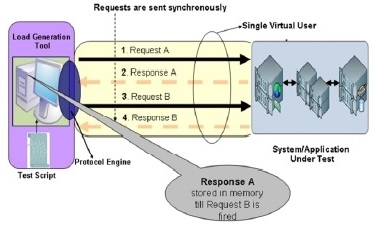
\includegraphics{images/architecture}
 \caption{Load testing tool architecture\label{fig:fig1_JMeter}}
\end{figure}\\
The protocol engine is synchronous in nature. By this we mean that for any virtual user
the requests are sent synchronously i.e. after firing the first request,  the protocol engine
waits for the corresponding response before firing the next request. Only after the next request is 
sent the response of the previous request which was stored in memory is discarded.\\
\\
On a given hardware, the maximum number of virtual users that can be simulated
is dependent on the average memory/CPU footprint for each virtual user which in turn
is dependent on the application response time and the complexity of the script.

\chapter{Design And Implementation}
 \section{Class Diagrams}
  \subsection{Assertions}
  \begin{figure}[H]
   \centering
   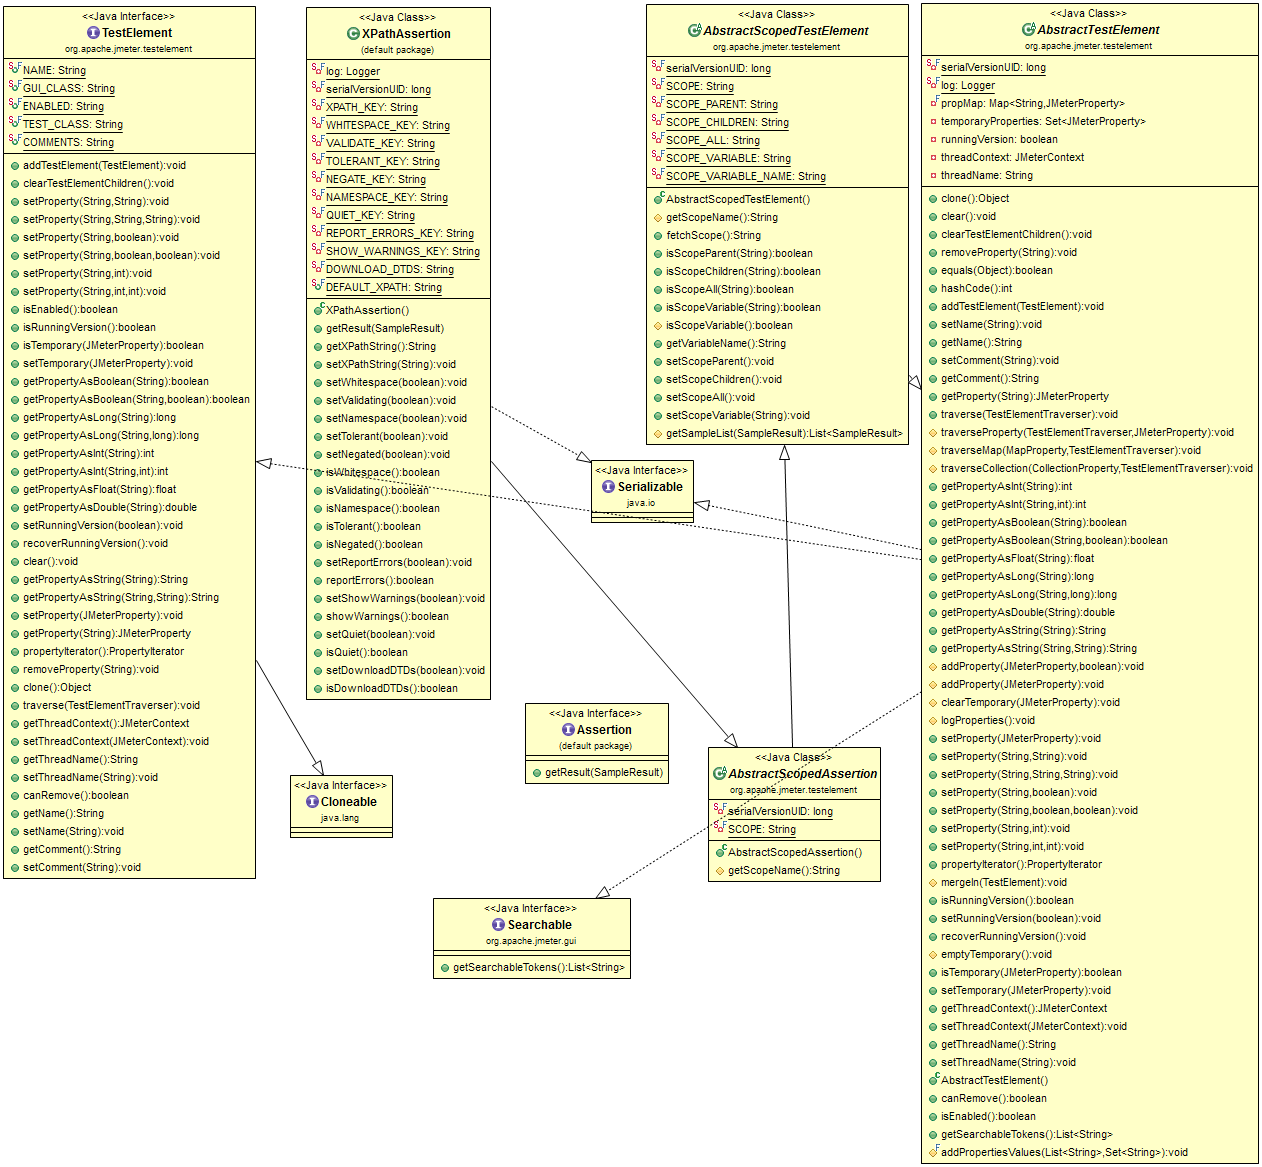
\includegraphics[width=17cm, height=16cm]{images/assertions_xpath}
   \caption{Class Diagram for XPath Assertion\label{fig:fig2_JMeter}}
  \end{figure}
  
  \begin{figure}[H]
   \centering
   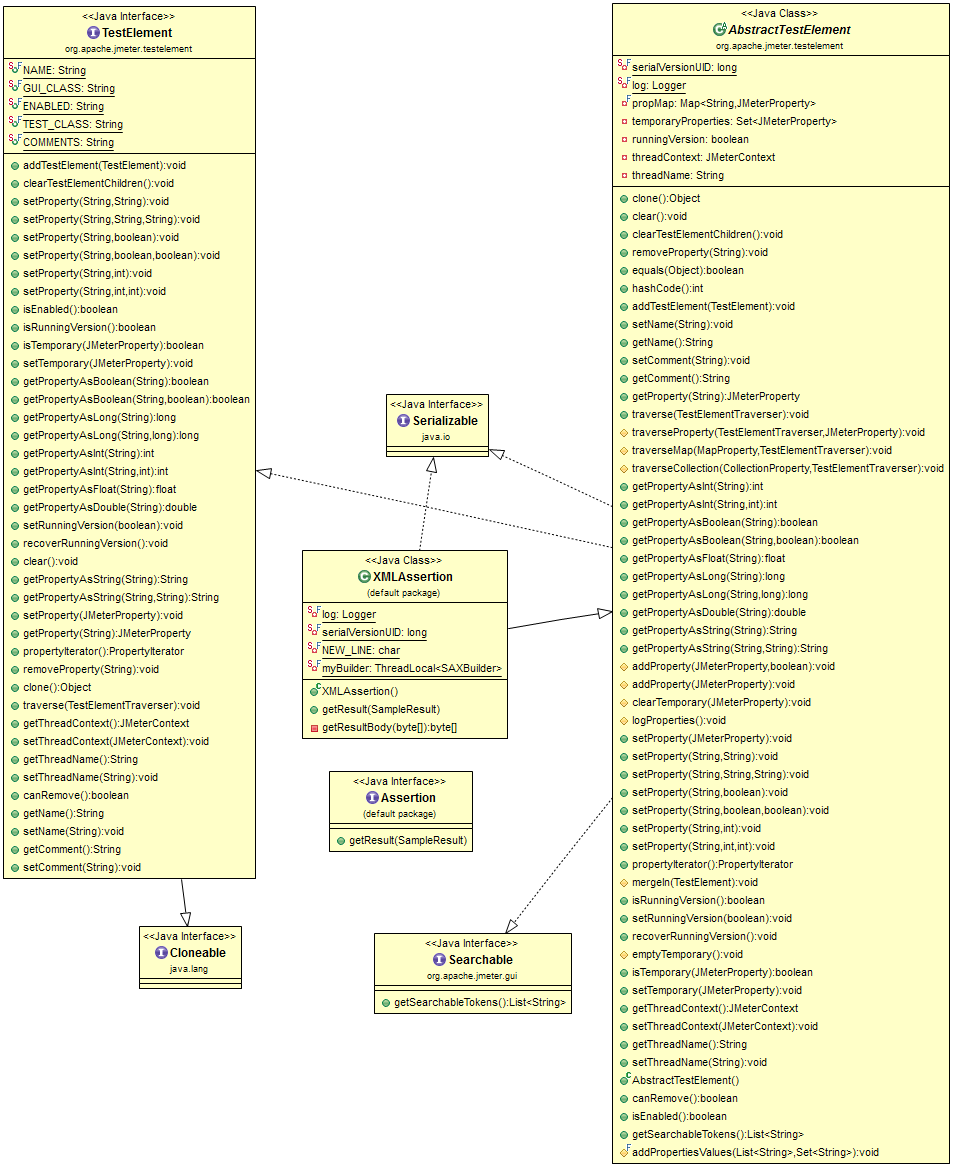
\includegraphics[width=17cm, height=22cm]{images/assertions_xml}
   \caption{Class diagram for XML Assertion\label{fig:fig3_JMeter}}
  \end{figure}
  
  \subsection{Configuration Elements}
  \begin{figure}[H]
   \centering
   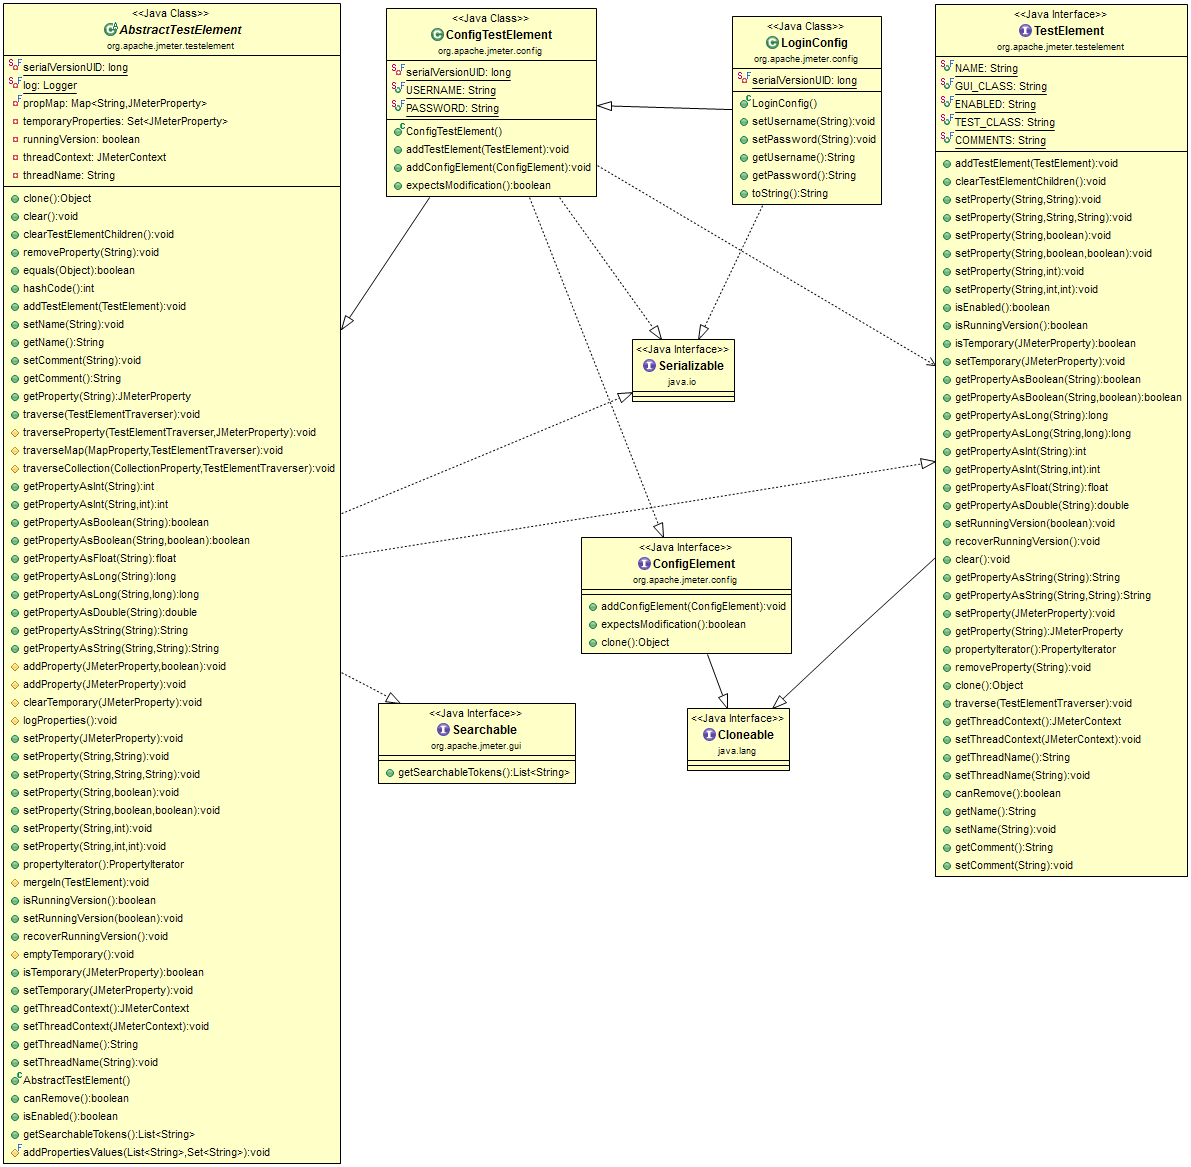
\includegraphics[width=17cm, height=22cm]{images/configelement_login}
   \caption{Class Diagram for Login Config element\label{fig:fig4_JMeter}}
  \end{figure}
  
  \begin{figure}[H]
   \centering
   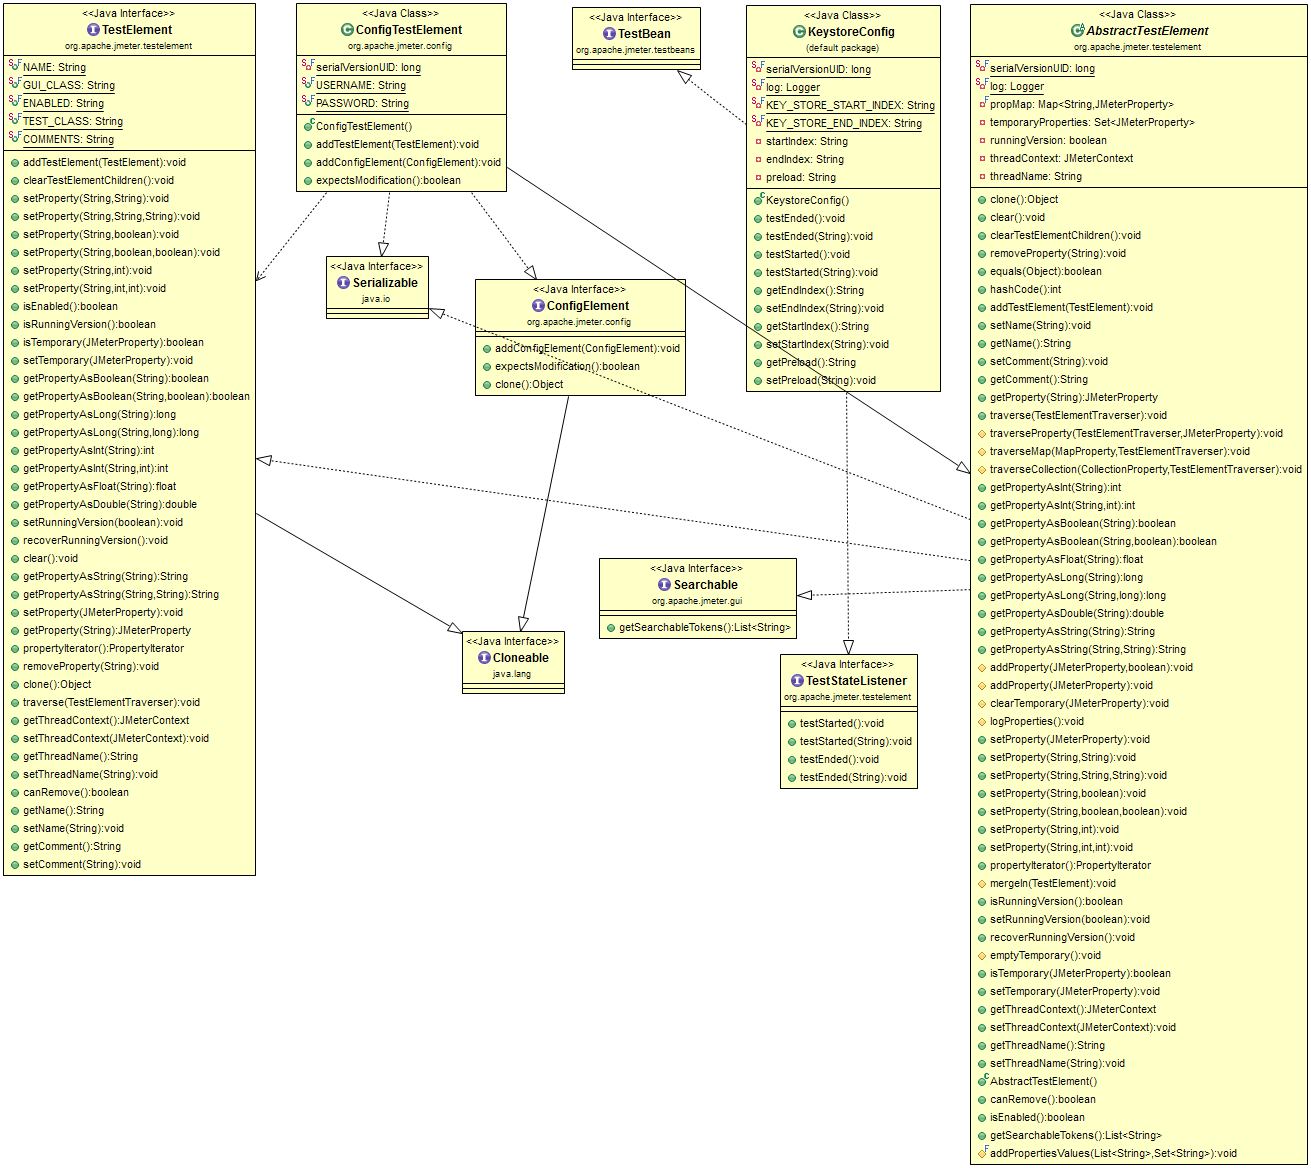
\includegraphics[width=17cm, height=22cm]{images/configelement_keyStore}
   \caption{Class Diagram for KeyStore Config\label{fig:fig5_JMeter}}
  \end{figure}
  
  \subsection{Logic Controllers}    
  \begin{figure}[H]
   \centering
   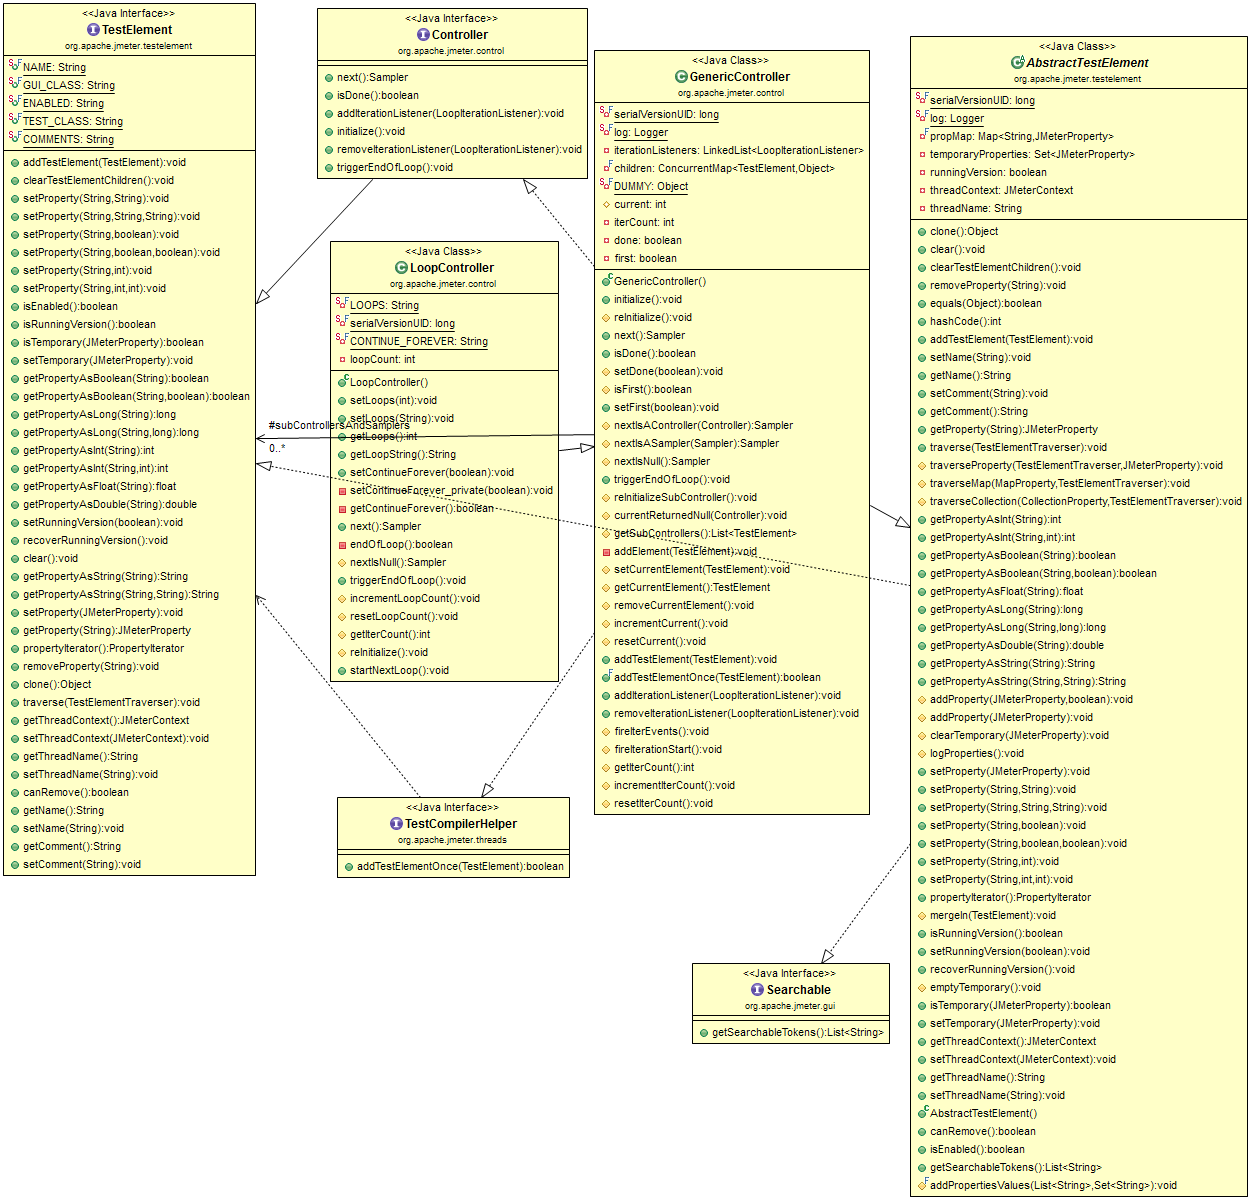
\includegraphics[width=17cm, height=22cm]{images/controller_loop}
   \caption{Class Diagram for Loop Controller\label{fig:fig6_JMeter}}
  \end{figure}
  
  \begin{figure}[H]
   \centering
   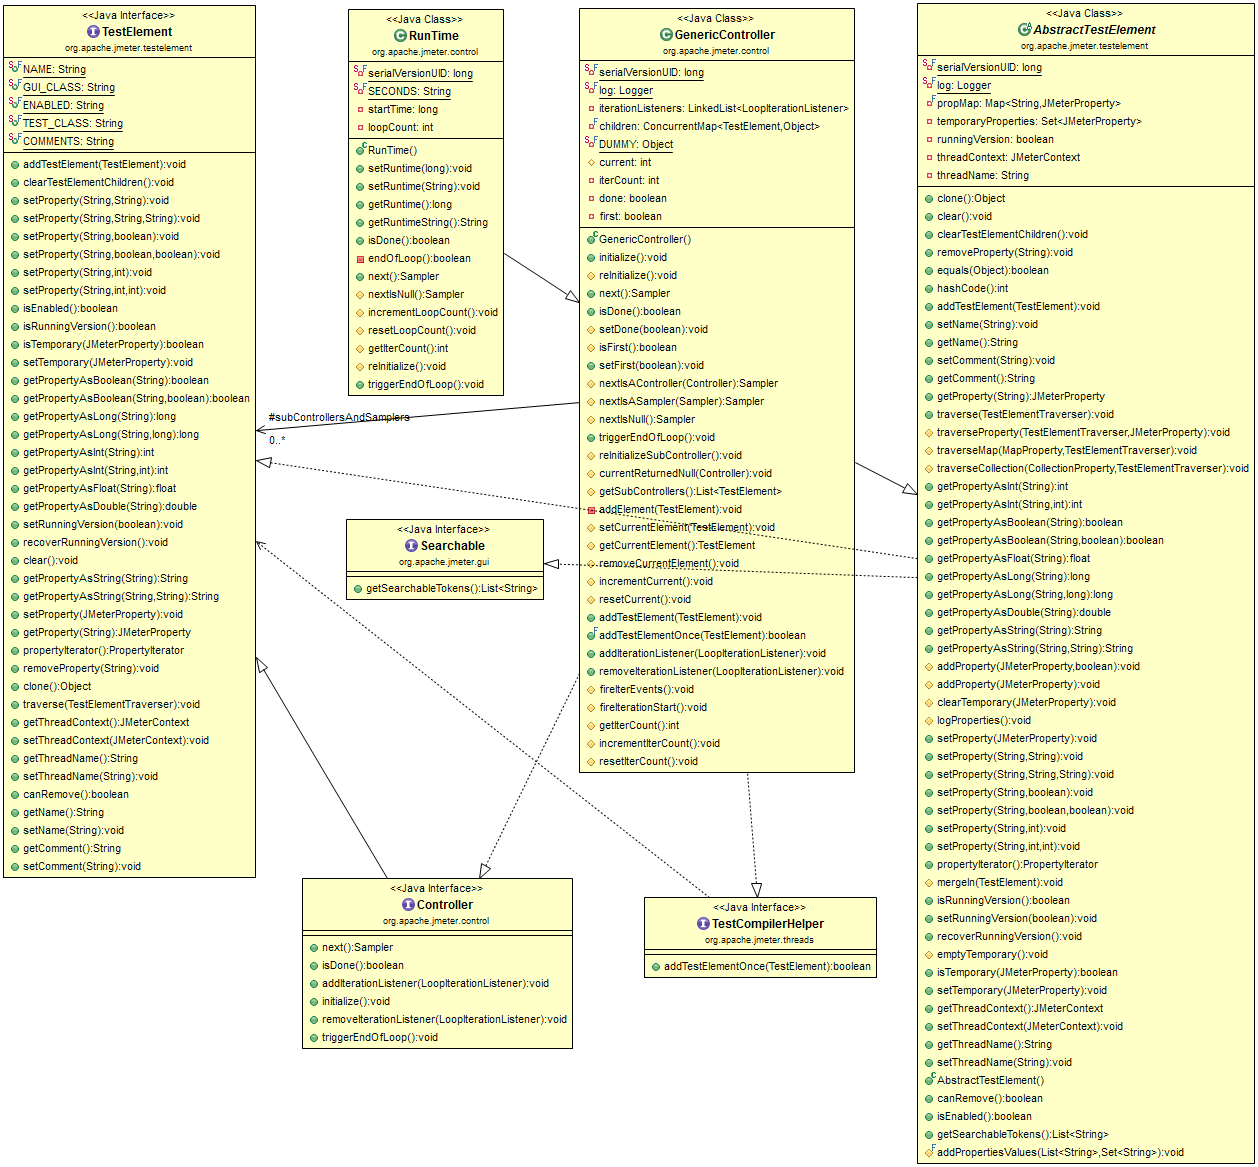
\includegraphics[width=17cm, height=22cm]{images/controller_runtime}
   \caption{Class Diagram for Runtime Controller\label{fig:fig7_JMeter}}
  \end{figure}
  
  \subsection{Post Processors}
  \begin{figure}[H]
   \centering
   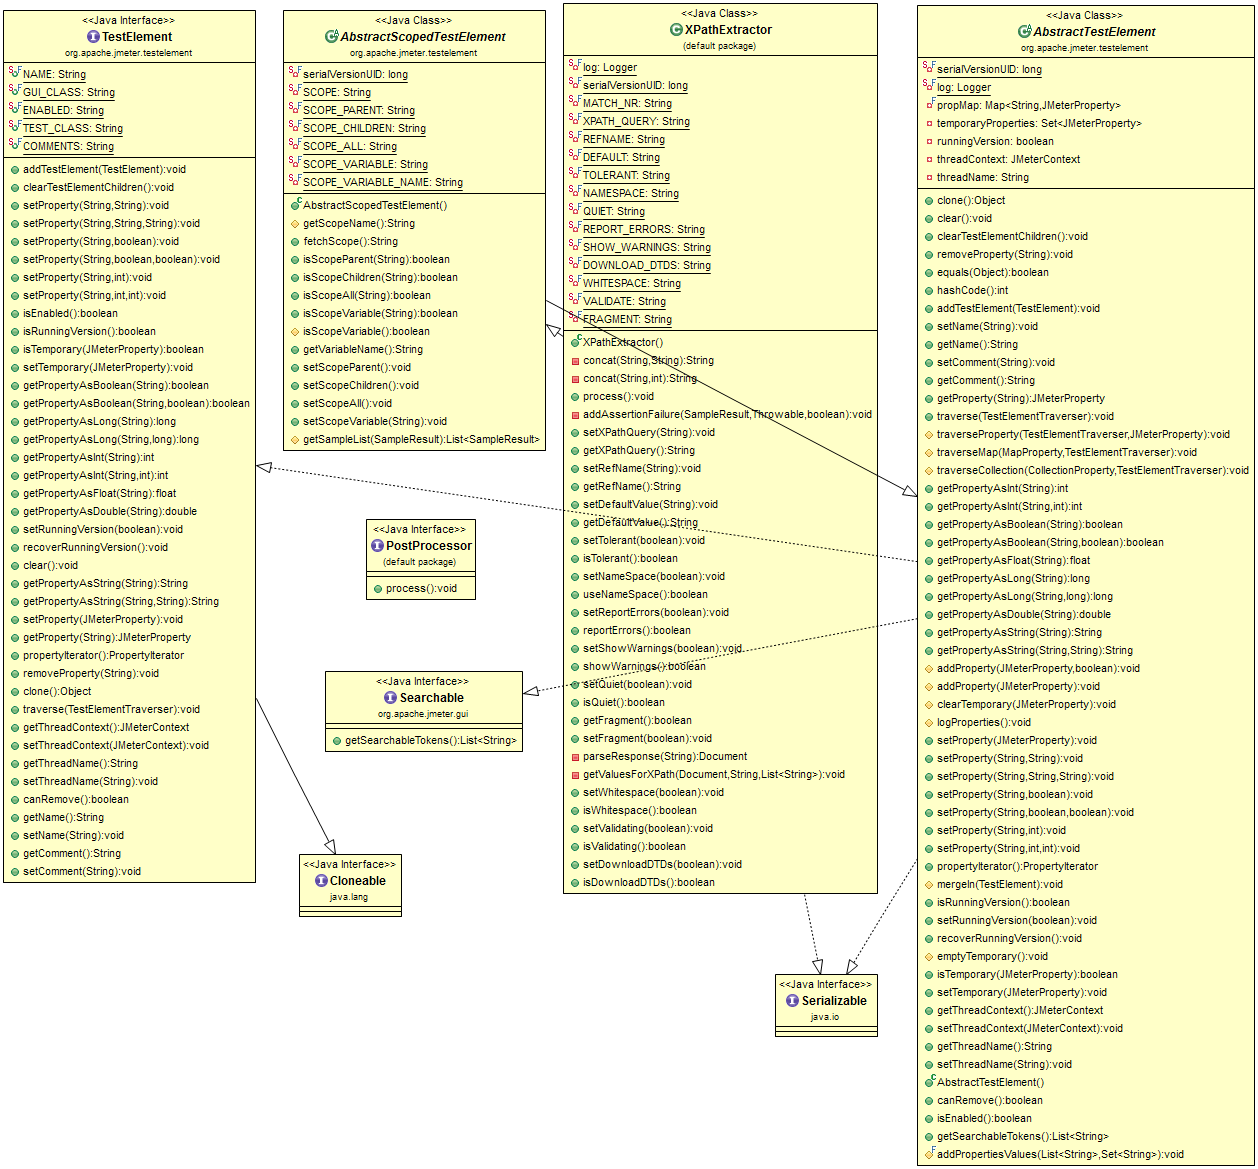
\includegraphics[width=17cm, height=22cm]{images/postprocessor_xpath}
   \caption{Class Diagram for XPath Extractor\label{fig:fig8_JMeter}}
  \end{figure}
  
  \begin{figure}[H]
   \centering
   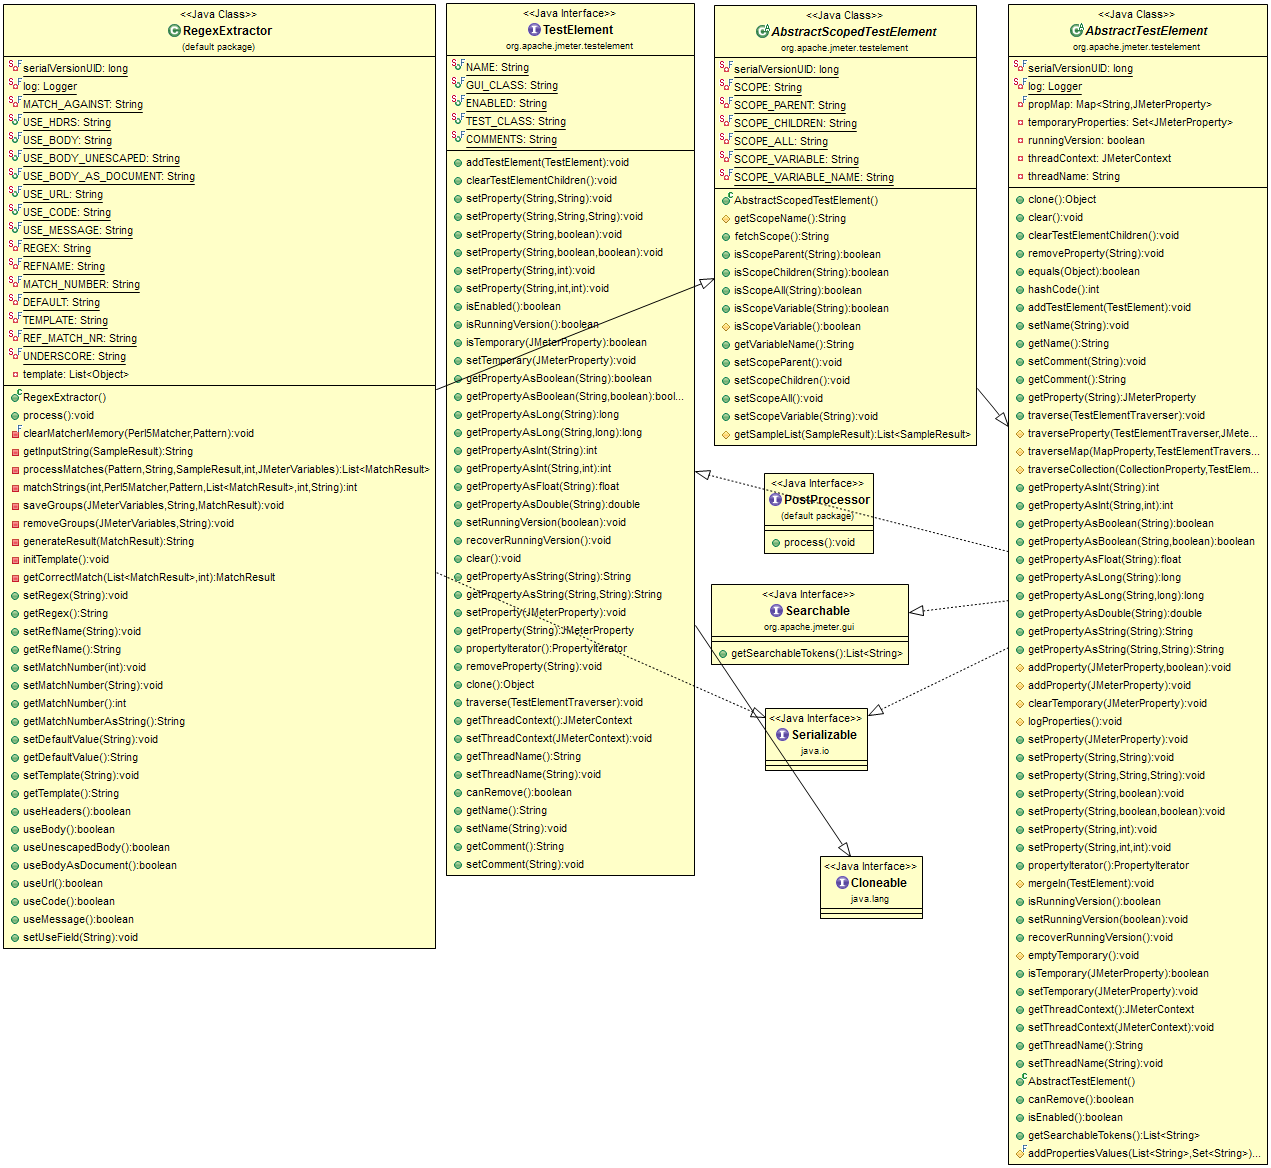
\includegraphics[width=17cm, height=22cm]{images/postprocessor_regex}
   \caption{Class Diagram for Regex Extractor\label{fig:fig9_JMeter}}
  \end{figure}
  
  \subsection{PreProcessors}
  \begin{figure}[H]
   \centering
   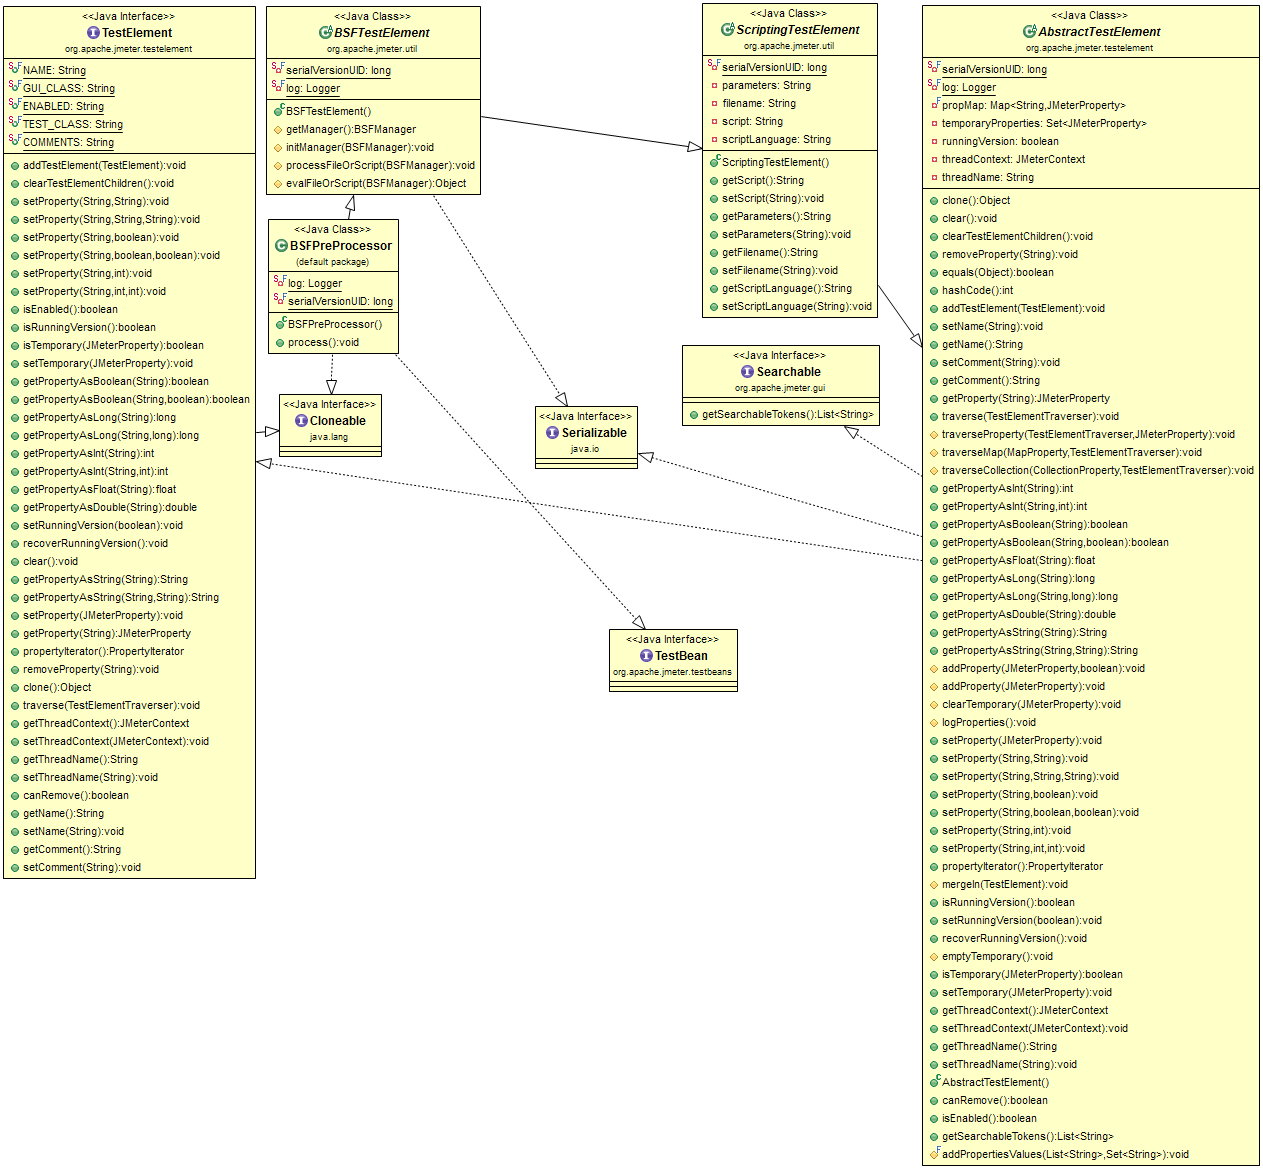
\includegraphics[width=17cm, height=22cm]{images/preprocessor_bsf}
   \caption{Class Diagram for BSF Preprocessor\label{fig:fig10_JMeter}}
  \end{figure}
  
\chapter{Detailed Description}
Apache JMeter consists of large number of components which are used in a variety of test plans.
These components have been categorised according to their use in the test plans like samplers are
used to define the work to be done by the virtual users and timers are used to set delay in the
execution of the samplers. Similarly there are pre-processors, post-processors, listeners, config
elements, assertions which have several elements under them. These elements are described in
detail in this section. Apart from these the newly added components have also been elaborated in
this section. Their functioning along with suitable examples are placed in the following sections. \cite{Ehh}

\section{Assertions}
Assertions are used to verify that the response of any samplers satisfies certain criteria.
If the criteria specified is met, it is a passed assertion, else the assertion is said to have failed.
This component is highly used in functional testing to check the responses received. Perl style regular 
expressions can be used to check the response data for some specified content. For eg. A “welcome” can be checked 
after a login window to check for successful login attempt. Assertions can be specified to be applied to either only
the samples to which they are added or to samples as well as sub-samples. \cite{Ehh} \cite{Jmeter} \cite{Manual}\\
\\
Types of assertions:   
 \subsection{Response Assertion}
 It is used to check if the response contains certain data or pattern.
 Either strings can be given to check if they are contained or matches the response, or 
 patterns can be specified with regular expression.
 
 \subsection{Duration Assertion}
 It is used to check that the response was received within a certain amount of time.
 
 \subsection{Size Assertion}
 This assertion can be used to check the size of the response data received, to be greater than, equal to or less than some specified size.
 
 \subsection{XML Assertion}
 This assertion is used to check that the response has formally correct XML. 
 
 \subsection{BeanShell Assertion}
 This component has facility to specify a beanshell script for checking the response.
 
 \subsection{MD5Hex Assertion}
 This assertion allows to specify a MD5Hex for the response to check its validity.
 
 \subsection{HTML Assertion}
 This assertion allows the checking of the response for correct HTML using JTidy.
 The minimum allowed errors and warnings found in the document can also be specified.
 
 \subsection{XPath Assertion}
 This assertion is used to check for a valid specified XPath in the response document.
 
 \subsection{XML Schema Assertion}
 This component can be used to check the response against an XML Schema.
 
 \subsection{BSF Assertion}
 This allows the specification of a BSF script code for asserting a sample.
 
 \subsection{JSR223 Assertion}
 This allows the specification of a JSR223 script code for asserting a sample.
 
 \subsection{Compare Assertion}
 This component facilitates the comparison of response results. The results can also be filtered out for some contents before performing the comparison. 
 
 \subsection{SMIME Assertion}
 This assertion is basically used with Mail Reader Sampler. The response can be checked to see if it has been signed or not, also validating 
 against a specific signature can be done.
 
\section{Configuration Elements}
Config Elements or Configuration elements are used to set defaults and variables to be used by
the samplers defined under their scope. There are 18 different config elements each for specific
purpose as described below.\cite{Ehh} \cite{Jmeter} \cite{Manual}

 \subsection{CSV Data Set Config}
 This config element is used to supply parameter values required
by different type of samplers in their requests. In this config element we supply a CSV file
containing parameter values and we specify the delimiter in the config element to separate the
combined set of values.

 \subsection{FTP Request Defaults}
 This config element is used to specify the default values to be
used by FTP samplers in their requests like server name or IP address, port number
method to be used get or post etc.

 \subsection{HTTP Authorization Manager}
 The authorization manager is used to specify one or more user logins for the web pages that are restricted using server authentication.
 
 \subsection{HTTP Cache Manager}
 This config element is used to add cache functionality to the
HTTP request samplers. If the previous sampler that requested some web page was successful
the Last-modified and E-tag parameters from the HTTP headers are saved for the urls. Later on
before requesting a page the cache is first checked if the value is their in the cache or not.

 \subsection{HTTP Cookie Manager}
 This config element is used to generate or to store cookies
for the users. If the response contains a cookie, that cookie is saved and is used for all future
references. Each thread have their own cookie storage, so we say if a cookie is used to maintain a
session then each thread runs in a separate session.

 \subsection{HTTP Request Defaults}
  This config element is used to set default values for the HTTP
samplers to be defined in its scope like server name or IP address or the port number,
parameters, method to be used , proxy configuration if any etc.

 \subsection{HTTP Header Manager}
 This config element is used to specify user defined values for
the parameters used in the HTTP headers like User-agents, accept-language etc.

 \subsection{Java Request Defaults}
 This config element is used to set default values for the java
requests samplers. Here we specify the parameters to be used in the java requests.

 \subsection{JDBC Connection Configurations}
 This config element is used to add default values for the JDBC connection samplers. In this element we can specify jdbc drivers, urls, connection
ports, connection pools, pool variable, pool time out etc.
 
 \subsection{Keystore Configurations}
 This config element is used specially with https samplers to establish secure connection that require exchange of encryption algorithms and keys to
be exchanged.

 \subsection{Login Config Element}
 This config element is used to override the login specification for a sampler in which scope this element is defined.
 
 \subsection{LDAP Request Defaults} 
 This element lets us set default values for LDAP testing like server name, port, distinguished name, test configurations etc.
 
 \subsection{LDAP Extended Request Refaults}
 This element is used for extended configuration to be used for LDAP testing search base, filter, scope, size limit, time limit, attributes etc.
 
 \subsection{TCP Sampler Config}
 This config element is used to set default values for TCP samplers like server name , port number, options like reuse connection close connection etc.
 
 \subsection{User Defined Variables}
 This element lets us define an initial set of variable. These variables are processed at the start of the test plan.
 
 \subsection{Random variable}
 Random Variable config element is used to generate random numeric strings and store them in variable for use later. They can be used in any specified format
as needed by the samplers.

 \subsection{Counter}
 This config element is used to create a counter that can be referenced anywhere in the thread group.
 This config element lets the user configure a start, maximum and increment values.
 
 \subsection{Simple Config Elements}
 The simple Config Element lets us add or overrode arbitrary values in the samplers. The users can choose a name of the value and value itself as required.
 
\section{Logic Controllers}
  Logic Controllers determine the ordering of the processing of the samplers  i.e. in what order the requests are sent to the server. \\
  There are 16 different logic controllers. They are:\cite{Ehh} \cite{Jmeter}\cite{Manual}
  \begin{itemize}
   \item Simple Controller 
   \item Loop Controller 
   \item Once Only Controller 
   \item Interleave Controller 
   \item Random Controller 
   \item Random Order Controller 
   \item Throughput Controller 
   \item Runtime Controller 
   \item If Controller 
   \item While Controller 
   \item Switch Controller 
   \item ForEach Controller 
   \item Module Controller 
   \item Include Controller 
   \item Transaction Controller 
   \item Recording Controller
  \end{itemize}

  \subsection{Once Only Controller}
  Controllers placed under the only once controller are processed only once per thread and any other 
  requests over further iterations are passed over. Eg. can be used with tests that require a login.
  
  \subsection{Loop Controller}
  Samplers placed within the loop controller will be looped the number of times specified in the GUI of 
  the controller in addition to the value specified for the thread group.
  
  \subsection{Interleave Controller}
  For each iteration the samplers placed within this controller are processed in an interleaved manner .

  \subsection{Random Controller}
  Similar to the interleave controller except the fact that the request instead of following a particular order are fired at random.
  
  \subsection{Random Order Controller}
  Similar to simple controller except the fact that the order of execution of the samplers is random.
  
  \subsection{Throughput controller}
  Throughput controller basically allows the user to control the number of executions of the samplers. There are two modes:
  \begin{itemize}
   \item Percent execution
   \item Total executions
  \end{itemize} 
  
  \subsection{If Controller}
  The If Controller allows the user to control whether the test elements below it (its children) are run or not depending on
  the condition being satisfied or not. 
  
  \subsection{While Controller}
    The controllers placed within this controller are fired until the loop condition becomes ‘false’.
  
  \subsection{Module Controller}
  The Module Controller provides a mechanism for substituting test plan fragments from other test plans  into the current test plan at 
  run-time providing the convenience of  running many alternate test plans quickly and easily
  
  \subsection{Include Controller}
  The include controller allows the user to  an external jmx file present in the bin directory of JMeter.
  
  \subsection{Transaction Controller}
  The Transaction Controller generates an additional sample which measures the overall time taken for the execution of the elements present within it.
  
  \subsection{Runtime Controller}
  The Runtime Controller controls how long its children are allowed to run depending on the time specified by the user in the given field. 
  
  \subsection{Switch Controller}
  Similar to the Interleave controller, except the fact that rather than running the subordinate elements present within it  in sequence it runs
  the elements defined by the switch value. 
  
  \subsection{Foreach Controller}
  A ForEach controller loops through the values of a set of related variables. 
  The input should consist of several variables, each extended with an underscore and a number.  
  
  \subsection{Recording Controller}
  The Recording Controller is a place holder indicating where the proxy server should record samples to.During recording using the HTTP Proxy Server \cite{Ehh},
  all recorded samples will by default be saved under the Recording Controller. 

\section{Post-Processors}
Post-processors are used to process some action after a sampler. They are executed after the sampler. They are applied only to the parent
samples.\cite{Ehh} \cite{Jmeter}\cite{Manual}

  \subsection{Regular Expression Extractor}
  It allows the user to extract values from the response of the sampler. A pattern can be specified which is to be found and values extracted from it.
  The extracted values can be stored in template strings or specified variables. A group of values can be extracted by this extractor for further use.
  
  \subsection{CSS/JQuery Extractor}
  It allows the extraction of values using a CSS/JQuery syntax from the response received.
  
  \subsection{XPath Extractor}
  This test element allows the user to extract value(s) from structured response - XML or (X)HTML - using XPath query language.
  
  \subsection{Result Status Action Handler}
  This component allows the specification of the action to be taken on the failure of a sampler.
  
  \subsection{BeanShell PostProcessor}
  It allows the specification of action to be taken in a BeanShell script, after the sampler has run.
  
  \subsection{BSF PostProcessor}
  It allows the specification of action to be taken in a BSF script, after the sampler has run.
  
  \subsection{JSR223 PostProcessor}
  It allows the specification of action to be taken in a JSR223 script, after the sampler has run.
  
  \subsection{JDBC PostProcessor}
  This component allows for the execution of some SQL statements just after a sample has run.
  It can be useful in cases where some changes made by the sample to the database needs to be undone after the sample has processed.
  
\section{PreProcessors}
  Preprocessors are used to modify the Samplers in their scope. There are nine types of preprocessors defined in JMeter.They are:\cite{Ehh} \cite{Jmeter} \cite{Manual}
  \begin{itemize}
   \item HTML Link Parser 
   \item HTTP URL Re-writing Modifier 
   \item HTML Parameter Mask 
   \item User Parameters 
   \item BeanShell PreProcessor 
   \item BSF PreProcessor 
   \item JSR223 PreProcessor 
   \item JDBC PreProcessor 
   \item RegEx User Parameters 
  \end{itemize}

  \subsection{HTML Link Parser}
  This modifier parses HTML response from the server and extracts links and forms. A URL test sample that passes through this modifier will 
  be examined to see if it "matches" any of the links or forms extracted from the immediately previous response. It would then replace the values
  in the URL test sample with appropriate values from the matching link or form. Perl-type regular expressions are used to find matches. Eg-Can be 
  used in “spidering” through a site. 
  
  \subsection{HTTP URL Re-writing Modifier}
  For web applications that use URL Re-writing to store session ids instead of cookies, the HTTP url re-writing modifier element can be attached 
  at the ThreadGroup level, much like the HTTP Cookie Manager . When given the name of the session id parameter, it finds it on the page and add
  the argument to every request of that ThreadGroup. 
  
  \subsection{HTML Parameter Mask}
  The HTML Parameter Mask is used to generate unique values for HTML arguments. By specifying the name of the parameter, a value prefix and suffix,
  and counter parameters, this modifier will generate values of the form " name=prefixcountersuffix ". Any HTTP Request that it modifies, it will replace 
  any parameter with the same name or add the appropriate parameter to the requests list of arguments. 
  
  \subsection{User Parameters}
  Allows the user to specify values for User Variables specific to individual threads. User Variables can also be specified in the Test Plan but not 
  specific to individual threads. This panel allows you to specify a series of values for any User Variable. For each thread, the variable will be assigned
  one of the values from the series in sequence. If there are more threads than values, the values get re-used. For example, this can be used to assign a 
  distinct user id to be used by each thread. 
  
  \subsection{JDBC Preprocessor}
  JDBC PreProcessor enables you to run some SQL statement just before a sample runs. This can be useful if your JDBC Sample requires some data to be 
  in DataBase and you cannot compute this in a setup Thread group.
  
  \subsection{RegEx User Parameters}
  Allows to specify dynamic values for HTTP parameters extracted from another HTTP Request using regular expressions. RegEx User Parameters are specific
  to individual threads. This component allows you to specify reference name of a regular expression that extracts names and values of HTTP request parameters.
  Regular expression group numbers must be specified for parameter's name and also for parameter's value. Replacement will only occur for parameters in the 
  Sampler that uses this RegEx User Parameters which name matches.
  
  \subsection{BeanShell Preprocessor}
  The BeanShell PreProcessor allows arbitrary code to be applied before taking a sample. \\
  
  Before invoking the script, some variables are set up in the BeanShell interpreter: 
  \begin{itemize}
   \item log - (Logger) - can be used to write to the log file 
   \item ctx - ( JMeterContext ) - gives access to the context 
   \item vars - ( JMeterVariables ) - gives read/write access to variables: vars.get(key); vars.put(key,val); vars.putObject("OBJ1",new Object()); 
   \item props - (JMeterProperties - class java.util.Properties) - e.g. props.get("START.HMS"); props.put("PROP1","1234"); 
   \item prev - ( SampleResult ) - gives access to the previous SampleResult (if any) 
   \item sampler - (Sampler)- gives access to the current sampler 
  \end{itemize}
  
  \subsection{BSF PreProcessor}
  The BSF PreProcessor allows BSF script code to be applied before taking a sample. \\
  The script (or file) is processed using the BSFEngine.exec() method, which does not return a value.\\
  The following BSF variables are set up for use by the script: 
  \begin{itemize}
   \item  log - (Logger) - can be used to write to the log file 
   \item Label - the String Label 
   \item Filename - the script file name (if any) 
   \item Parameters - the parameters (as a String) 
   \item args[] - the parameters as a String array (split on whitespace) 
   \item ctx - ( JMeterContext ) - gives access to the context 
   \item vars - ( JMeterVariables ) - gives read/write access to variables: vars.get(key); vars.put(key,val); vars.putObject("OBJ1",new Object()); vars.getObject("OBJ2"); 
   \item props - (JMeterProperties - class java.util.Properties) - e.g. props.get("START.HMS"); props.put("PROP1","1234"); 
   \item sampler - (Sampler)- gives access to the current sampler 
   \item OUT - System.out - e.g. OUT.println("message") 
  \end{itemize}
  
  \subsection{JSR223 Preprocessor}
  The JSR223 PreProcessor allows JSR223 script code to be applied before taking a sample.
  
\section{Timers}
  Usually in JMeter the request from the threads are obtained without any time lapse between them. This in turn causes the increase of load factor on the server.
  To eliminate such phenomena we have the concept of Timers. \cite{Ehh} \cite{Jmeter}\cite{Manual}\\
  \\
  The Timers eliminate the overload by adding delay between each request.

  \subsection{Constant Timer}
  As its name suggests this timer adds same amount of delay between requests.
  
  \subsection{Gaussian Random Timer}
  The Gaussian random timer inserts random delays between requests of almost same amount of time.\\
  The total delay is the sum of the Gaussian distributed value (with mean 0.0 and standard deviation 1.0)
  times the deviation value you specify, and the offset value. 
  
  \subsection{Uniform Random Timer}
  This timer pauses each thread request for a random amount of time, with each time interval having the same probability of occurring.
  
  \subsection{Constant Throughput Timer}
  The constant throughput timer is dependent on the system’s throughput. It inserts variable delays to keep the systems throughput constant.
  
  \subsection{Synchronising Timer}
  The SyncTimer is to block threads until X number of threads have been blocked, and then they are all released at once. 
  A SyncTimer can thus create large instant loads at various points of the test plan.
  
  \subsection{BSF Timer}
  BY using BSF(Bean scripting framework) scripting language we can be generate delays.
  
  \subsection{Beanshell Timer}
  Beanshell is a lightweight scripting for java which is used to generate delays.
  
  \subsection{JSR223 Timer}
  JSR223 is a scripting language developed by java platform which is used to generate delays.
  
  \subsection{Poisson Random Timer}
  The Poisson random timer inserts random delays between requests of almost same amount of time.\\
  The total delay is the sum of the Poisson distributed value, and the offset value.
  
\section{Visualizers/Listeners}

  Listeners are an integral component of any test plan, without Listeners one cannot analyze the results of a test. 
  The basic Listener “Simple Data Writer” records all the data in CSV or XML format and stores it for suther reference. 
  The Simple data writer is preferably used in non-GUI mode, as it saves the overhead of GUI functionality. \\
  \\
  Listeners are prepped at the bottom of the scope in which they are kept.\\
  Listeners can use a tonnes of memory space if the number of samples is huge.\cite{Ehh} \cite{Jmeter} \\
  \\
  List of Listeners in JMeter:
  \begin{itemize}
   \item Sample Result Save Configuration
   \item Graph Results
   \item View Results Tree
   \item Monitor Results
   \item Aggregate Report
   \item Spline Visualizer
   \item Assertion Results
   \item View Results in Table
   \item Simple Data Writer
   \item Distribution Graph (alpha)
   \item Response Time Graph
   \item Aggregate Graph
   \item Mailer Visualizer
   \item BeanShell Listener
   \item Summary Report
   \item JSR223 Listener
   \item Generate Summary Results
   \item Save Responses to a file
   \item BSF Listener
   \item Comparison Assertion Visualizer
  \end{itemize}
 
 \subsection{Graphical Listeners}
 These category of Listeners produce graphical results of the samples response and other parameters like Latency, Percentage error, etc.
 The graph results Listener plots a graphs of Response time, also calculating Average, Median, Deviation and Throughput.
 The spline visualizer divides the data into to parts and takes an average of each part. These 10 points are plotted and a spline curve is drawn 
 using these 10 points. The aggregate graph plots a bar graph of aggregate response of each sampler in each thread group. The response time graph 
 provides neat results of just the response time of each sample. The Monitor results Listener monitors the load on server side, calculating Memory and 
 CPU usage and warns of overload. The Distribution Graph Listener draws a graph based on response time of samples, showing how many samples were below 
 average of 50\% and 90\% lines.
 
 \subsection{Tabular Results Listeners}
 These Listeners produce results in a tidy table format. The View results in table Listener gives the Start time, Thread name, Sample time,
 Status, Size (in Bytes) and Latency. The Aggregate report provides Median, 90\% Line, Mininmum and Maximum, Throughput and Error percentage 
 for each Sampler. Summary reports give an overall summary of result data collected from the test.
 
 \subsection{Assertion Results}
 The Assertion Results visualizer is used to check assertion of any sampler. It also reports non-performing Assertions that are part of the test plan.
 
 \subsection{View Results Tree}
 The View Results Tree displays a tree-like hierarchy of all sample responses, allowing the tester to view the response for any sample. 
 In addition to displaying the response, one can view the time it took to fetch this response, and some response codes.
 
 \subsection{Mailer Visualizer}
 The mailer visualizer serves the purpose of setting up to email if a test run gets too many failed responses from the system or server.
 
 \subsection{BeanShell Listener}
 The BeanShell Listener provides the use of BeanShell for checking samples for saving etc.
 
 \subsection{BSF Listener}
 The BSF Listener provides the functionality of BSF script code to be applied to sample results.
 
 \subsection{JSR223 Listener}
 The JSR223 Listener makes the JSR223 script code to be applied to sample results.
 
 \subsection{Comparison Assertion Visualizer}
 The Comparison Assertion Visualizer displays the results of Compare Assertion elements.
 
\section{Samplers}
  Samplers are the components of JMeter that decide the action of the virtual users in a test plan. Samplers generate different types of sample 
  results which have various attributes like time elapsed,  success,  fail,  data size etc. These results can be viewed in various listeners.\\
  
  There are 21 types of samplers present in JMeter. Some of them are described as follows:\cite{Manual}
  

  \subsection{FTP Request}
  This sampler component lets the user send an FTP "download file" or "upload file" request to an FTP system server.
  
  \subsection{HTTP Request}
  This sampler component lets the user send an HTTP request or a HTTPS request to a web server. This sampler also lets the user modify whether 
  or not JMeter fetches HTML files for images and other embedded resources and sends HTTP requests to retrieve them.
  
  \subsection{JDBC Request}
  This sampler component allows the user send a JDBC Request (an SQL query) to a server having a database. If the Variable Names list is given,
  then for every   row returned by a Select statement, the variables are put up with the value of the corresponding column.
  The number of rows is also set.
  
  \subsection{Java Request}
  This sampler component permits the user to control a java class that implements the org.apache.jmeter.protocol.java.sampler.JavaSamplerClient
  interface from JMeter source code.

  
  \subsection{SOAP/XML-RPC Request}
  This sampler component allows the user to send a SOAP request to a website haivng the SOAP webservice. It can also be modified to send a XML-RPC
  packet over HTTP packets. It creates an HTTP POST request, with the specified XML as the POST content. 
  
  \subsection{LDAP Request}
  This Sampler component gives a interface to the user to send a different Ldap request(Add, Modify, Delete and Search) to an LDAP server.
  There are two ways to generate test cases for the purpose of testing an LDAP Server.
  \begin{enumerate}
   \item Inbuilt Test cases.
   \item User defined Test cases.
  \end{enumerate}


  
  \subsection{Access Log Sampler}
  AccessLogSampler was developed to review access logs and create http requests. The latest implementation of AccessLogSampler prioritizes the
  creator to generate a new HTTPSampler. The servername, port and get images are specified by AccessLogSampler. Next component, the parser is 
  called with integer 1 as the parameter, telling it to parse only one entry. Then, HTTPSampler.sample() is used to set the request.
  
  \subsection{BeanShell Sampler}
  This sampler components permits the user to create a sampler using the BeanShell scripting language. The test element is compatible with the 
  ThreadListener and TestListener interface methods. These have to be defined in the initialisation file.
  
  \subsection{BSF Sampler}
  This sampler component gives the user interface to use a sampler using a BSF scripting language. By default, JMeter has support for the 
  following languages:
  \begin{enumerate}
   \item Javascript
   \item Jexl (JMeter version 2.3.2 and later)
   \item Xslt
  \end{enumerate}

  
  \subsection{JSR223 Sampler}
  The JSR223 Sampler component permitss JSR223 script code to be executed to perform a sample. JSR223 related components have a feature that highly 
  increases their performances.
  
  \subsection{TCP Sampler}
  The TCP Sampler component creates a TCP/IP connection to the given server. It then requests the text, and waits for a response. 
  Different hosts/port coloumn combinations will use distinct connections, as will distinct threads.
  
  \subsection{JUnit Request}
  The latest implementation of this component supports standard Junit convention and extensions. It also has extensions like the
  oneTimeSetUp and the oneTimeTearDown. The sampler component works like the JavaSampler with some differences.
  
  \subsection{Mail Reader Sampler}
  The Mail Reader Sampler component can read (and optionally delete) mail messages on server using POP3(S) or IMAP(S) protocols. 
  Mail Messages are kept as subsamples of the main sampler.
  
  \subsection{Test Action}
  The Test Action sampler is a sampler component that is used in a conditional controller. Rather than generating a sample, the test
  element eithers endures a pause or stop on the selected target. This sampler component can also be very useful in comparison with the 
  Transaction Controller, as it permits pauses to be instilled without requiring to create a sample.
  
  \subsection{SMTP Sampler}
  The SMTP Sampler component can send mail messages using SMTP or SMTPS protocol. It is also possible to allow security protocols 
  for establishing the connection (SSL and TLS) with the server, as well as for the user authentication.
  
  \subsection{OS Process Sampler}
  The OS Process Sampler component is a type of sampler component that can be put to use to execute commands on the a 
  system machine terminal. This sampler component allows execution of any command that can be executed from the command line.
  
\section{Auto CSV Generation}
For any tester testing with a large number of users; on an application which has a form or
request that takes multiple data entries and the data entries are required to be unique for different
users; it becomes a redundant work to type .csv files with unique data set entries. But,
necessarily, the back end Database of the AUT, which already contains this data for a number of
users, is available with the tester and he would like to use this file instead of creating ``Comma
Separated File'' for this purpose. The main aim of the ``Auto CSV Generation'' is to automate the
generation of the .csv file from the mentioned table of the Database, to be used with samplers.\\

For this purpose, the ``Auto CSV Generation'' is used as a non test element, before setting
up the actual experiment. The ``Auto CSV Generation'' is added to the Test Plan of JMeter and
the connection details of the DBMS used with username and password, the Database and the
table for which .csv is to be created, is specified. Then the plan is played, without the actual test
elements.\\

Thus the table mentioned is saved in form of .csv file, with each row of the table, as a set
of comma separated data. The new .csv file is named as ``databaseName\_tableName.csv'' and can
be found in the ``bin'' folder of the JMeter.\\

This .csv file can now be used in the pre-existent config element ``CSV Data Set
config'' and the variables of the ``CSV Data Set config'' can be related to the values of parameter
of the sampler. Now the ``CSV Data Set config'' is made the child of respective sampler, so that
the sampler can use the data in the .csv file, to send request to respective application, each time
representing a unique user, as the form data will be uniquely taken from .csv file and not
redundant.\\

\section{Filtered Results Listener Plugin}
The Filtered results Listener plugin works as an add-on to ``View Results in Table''
Listener in JMeter. The plug-in has a wide spread application in performance testing and load
testing, also in benchmarking any system.\\

When the user wants to set a filter on any value, he specifies a non-zero integer in the test
box and runs the test, as the tables are populated; only the values greater/less than specified value
will be displayed in the table. The utility of such results is the clarity it provides in performance
testing of system under test. Only those results satisfying the condition selected will be
displayed.\cite{Manual}

\section{SMTP Defaults}
Configuration Elements or config elements are important component of the test plans designed in
Apache JMeter. They are mainly used to specify default values or variables to be used in the test
plan. This helps in preventing the redundant specification of the values to be used by the
samplers in the test plan.\\

The existing JMeter have several config element like Http Request Defaults which is used with
http request samplers, Java Request Defaults which is used with Java request samplers, Ldap
Request defaults, TCP Sampler config, JDBC Connection configuration which are all used for
specific purposes. The existing version of JMeter has a sampler called SMTP Sampler which is
used for testing smtp mail servers. There is large number of fields to be specified within sampler
before the test can be run, like Server or IP address of the SMTP server, the port address of the
smtp server, the mail address where the mail is to be sent, mail address of the person sending the
mail, the mail addresses where the copies of the mail is to be sent. In the authorization settings, if
required, the user-name and the password is to be specified. In the message settings the subject
of the mail, headers to be added, message to be sent, any attachment to be sent along with the
mail and other optional parameter which may or may not be selected depending upon the
configuration of the mail server to be tested.\\

In case if the test plan is having more than one sampler, like four or five or more, these data and
settings have to be specified for all the samplers which is too cumbersome as well as several
entries in the samplers are common which make these entries redundant. In this situation, there is
a need of a SMTP config element where default values can be set and these values need not be set in the samplers to be used.\\

Smtp Defaults Config Element is a configuration element that can be used to set default values
for Smtp samplers.\cite{Plugins}\cite{Plugins1}


\section{Automating TPC-C Tests in JMeter}
  TPC-C is a standard database server benchmark for transaction processing. It is used by companies to benchmark their servers for performance showcase.
  The benchmarking is carried out by OLTP(Online transaction processing) transactions on the database and calculating the rate of these transactions. \\
  TPC-C benchmarking ensures that the server fulfills some basic functionality of transaction processing irrespective of hardware and software requirements. 
  TPC-C includes creation of the database according to a scaling factor and then firing transaction procedures against it in a predefined manner.[3]\\
  
  \subsection{The Benchmark Model}
  TPC-C simulates the scenario of any supplier or company which has to sell, manage and distribute their products. 
  It is basically a scenario where a number of concurrent users execute transactions against this company’s server. 
  The transactions emulate the common and required activities of placing a new order, making payment, checking the order status, etc.
  The TPC-C benchmarking model can be illustrated with the following diagram\cite{Bench}\cite{Standard}\cite{Tpcc-pdf}

  \begin{figure}[H]
   \centering
   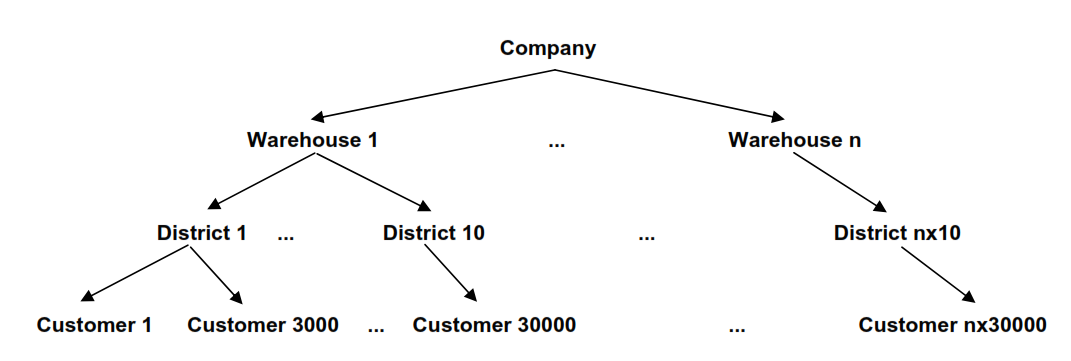
\includegraphics[width=17cm, height=6cm]{images/tpcc_intro1}
   \caption{Illustration of TPC-C benchmarking model\label{fig:fig11_JMeter}}
  \end{figure}
  
  The scenario is illustrated as a company having n number of warehouses.
  Each warehouse serves 10 districts. Each district has 3000 customers. The number of items held by the company is fixed to 1000,000 items.
  To manage this scenario the following database schema is being followed-\\
  

  \begin{figure}[H]
   \centering
   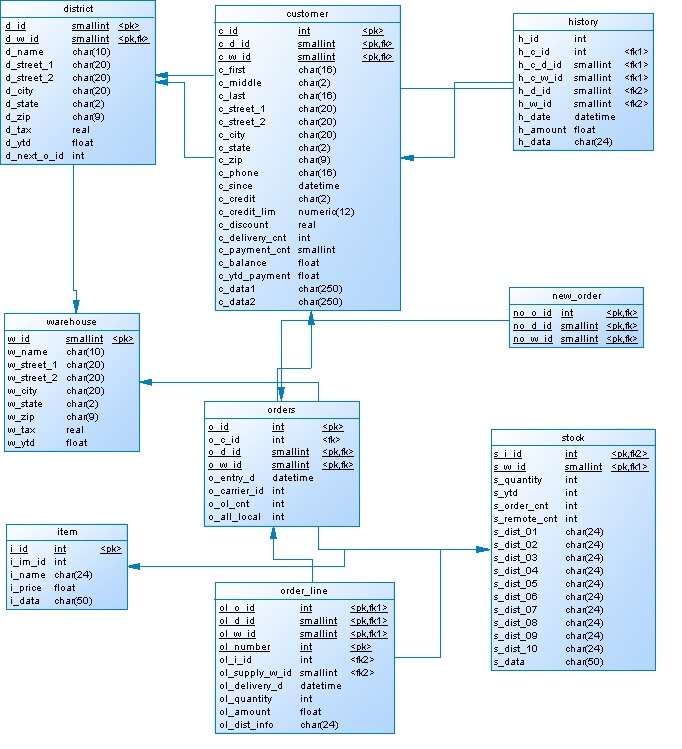
\includegraphics[width=17cm, height=20cm]{images/tpcc_intro2}
   \caption{Database Schema for TPC-C Benchmarking\label{fig:fig12_JMeter}}
  \end{figure}

The database consists of 9 tables. The names of the tables with the cardinality is given below\cite{Standard}:
 
 \begin{table}[H]
  \begin{center}
   \begin{tabular}{|c|l|p{9cm}|} 
   \hline
   \textbf{Sl No.} & \textbf{Table Name} & \textbf{No. of Rows}\\
   \hline
   1 & Item table & 100,000 rows(fixed) \\
   \hline
   2 & Warehouse table & 1 row for each warehouse \\
   \hline
   3 & District table & 10 rows for each warehouse\\
   \hline
   4 & Customer table & 30,000 rows for each warehouse\\
   \hline
   5 & History table & 30,000 rows for each warehouse \\
   \hline
   6 & Order table & 30,000 rows for each warehouse \\
   \hline
   7 & Orderline table & A mean value of 300,000 rows for each warehouse\\
   \hline 
   8 & New-Order table & 9,000 rows for each warehouse\\
   \hline
   9 & Stock table & 100,000 rows for each warehouse. \\
   \hline    
   \end{tabular}
   \caption{Database tables for TPC-C benchmarking}
  \end{center}
 \end{table}
 
The creation of one warehouse produces approximately 120 MB of data. 
The scaling factor of this database is the number of warehouses which the user specifies and accordingly the database is populated.
 The number of warehouses emulates the size of the company.
 The population of the database needs to follow some predefined functions by which the rows and columns of the database are filled up.
 The transactions to be carried out against this database also has some predefined procedures to be created and called.
 The 5 transactions carried out by the emulated user is-\\
 New Order Transaction\\
Payment Transaction\\
Order Status Transaction\\
Delivery Transaction\\ 
Stock level Transaction\\
In a practical scenario, the first two transactions are much more frequently carried out compared to the remaining three.
 So, the transactions are weighed such that, for each new order transaction there is one payment transaction to be carried out
 and for every 10 new order transaction, there will be one Delivery, Stock Level and Order Status transactions.\\ 
 All the 5 transactions are available at each terminal to be carried out by the emulated users.
 The transactions perform insert, update, delete on the database tables.
 These 5 transactions cover the basic business activities of any company.\\
The diagram below demonstrates an emulated TPCC test scenario:

  \begin{figure}[H]
   \centering
   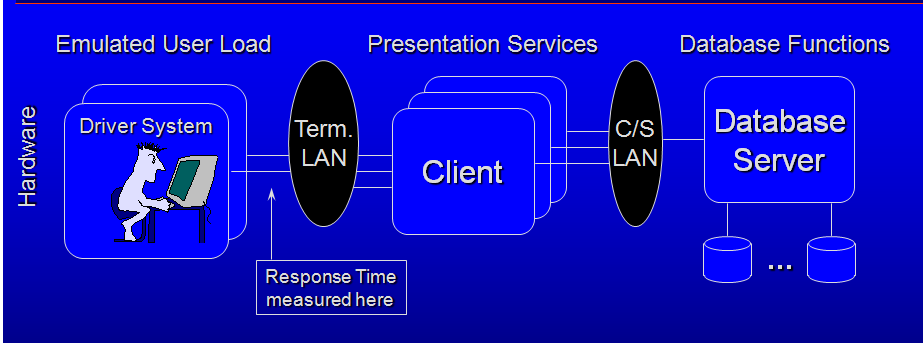
\includegraphics[width=14cm, height=6cm]{images/tpcc_intro3}
   \caption{TPC-C Test Scenario\label{fig:fig13_JMeter}}
  \end{figure}
  
The emulated users are the actual load to be produced. \\
The diagram below shows an example TPCC workflow:
  \begin{figure}[H]
   \centering
   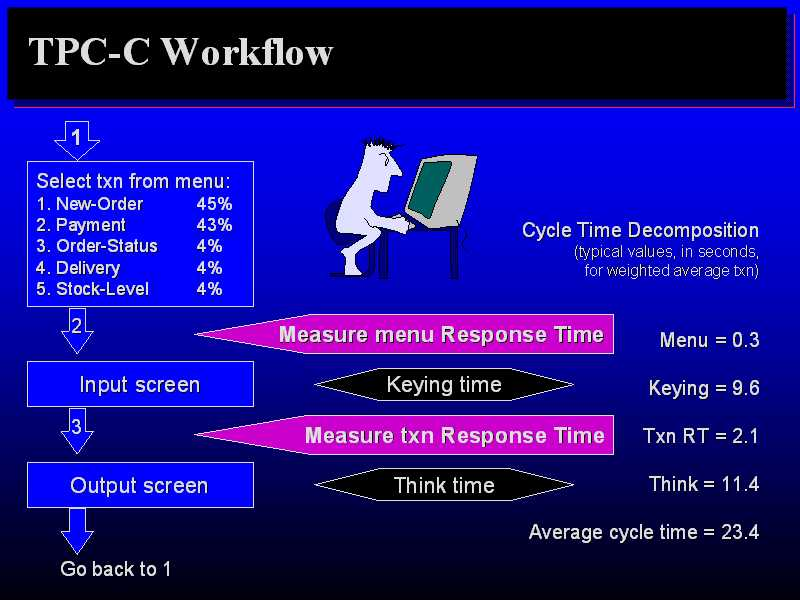
\includegraphics[width=14cm, height=7cm]{images/tpcc_intro4}
   \caption{TPC-C Workflow\label{fig:fig14_JMeter}}
  \end{figure}

  As illustrated by the figure, an activity is selected by the emulated user at the terminal.
  The data for the transaction is entered and the transaction begins.
  From the time the transaction begins till the complete output has been displayed to the screen, is measured as the transaction response time.
  The think time and the keying time are also included in the test scenario to make the testing scenario more practical.
  The think time is the time taken by the user to select the next transaction after the completion of one transaction.
  The keying time is the time taken by the user to enter the input data required by the transaction.\\
  As the transactions are carried out, the ACID properties of the database also need to be checked.
  Input values leading to rollback of transactions are also emulated.\\
  The calculated metric is \textbf{tpmC}.\\
  It is the number of new order transactions completed per minute. It is a measure of business throughput activities. \\



Detail on Transactions to be carried out\cite{Tpcc}\cite{Standard}:
 \begin{enumerate}
  \item \textbf{New Order transaction} \\
  It emulates a user placing a new order. The new order consists of approximately 10 items.
  1% of the orders in this transaction have invalid input numbers to exercise the rollback of transactions on the database.
  The new order item entry in made in the order, order\_line and new\_order tables.
  Also, a number of selections and updates take place in this procedure. \\

  \item \textbf{Payment transaction} \\
   It emulates the payment made by the customer. The balance of the customer is updated along with the statistics of the sales warehouse and district.\\ 
  
  \item \textbf{Order Status transaction} \\
  It is a read only transaction that shows the status of the last order placed by the customer. The customer may be identified by the customer id or the customer last name.\\
  \item \textbf{Delivery transaction} \\
    The delivery transaction deletes rows from new\_order and updates the corresponding orders and order\_line tables.
	It is fired every 10 new order transactions and processed for all ten districts in a loop.\\ 
  \item \textbf{Stock Level transaction} \\
  It consists of a heavy read only transaction.
  It basically selects the number of items that were recently sold and whose stock level is below a certain threshold.\\
 \end{enumerate}
 
\section{Bandwidth Throttling}
Bandwidth throttling is the slowing of Internet service provided to the users intentionally. This process is
employed in the communication networks to regulate the network traffic, hence bandwidth is minimized to control congestion.\\

Throttling can be used to limit a user's data access rates (upload and download) on programs such as
torrents clients, video streaming and other file sharing applications. It can be used to even out the
total bandwidth usage supplied across all users on the network as well. Bandwidth throttling is
also used in various Internet applications to avoid overloading individual servers or to spread the load over a wider network to reduce
local network congestion, for reducing the risk of server crashing.\\

\textbf{Utility of bandwidth throttling in JMeter}\\
JMeter is a testing tool employed to test web services under various loads, configurations,
situations, and environment. In the real world scenario, the web services are used by a vast
variety of users using different categories of network connections. Some people use extremely
high broadband connection while some use low bandwidth mobile connections to use various
web services. For example, the railway ticket booking website, IRCTC deals with millions and
billions of simultaneous requests at the same time from a vast number of users from all across
India. Similarly major social netwoking websites are used by even greater number of users from
all across the globe. So in there is a need to test these services from users using different
available bandwidth. Such tests can provide the usability, scalability of the servers under
different network connections. Such test can help is the recognizing the scenarios in which the
service is unusable or to test the minimum requirement to use the service. Such functionality in
JMeter can increase its usability in testing web services where the tester can specify the available
bandwidth which can less than or equal to the available bandwidth to the system and JMeter will
use this bandwidth to send or receive requests to/from the servers. JMeter can measure the
response time, throughput, amount of data exchanged, latency and errors in the transaction using
variable bandwidth as required the scenario described above.\\
Bandwidth throttling can be used with IP spoofing to create a test plan simulating a real world
scenario where users try to access a web service from various geographical locations having a
varying bandwidth and using different IP addresses which makes the test plan more realistic and
reduces the use of multiple system for testing.\cite{Comp}

\section{Dynamic Bandwidth Throttling}
Dynamic Bandwidth Throttling deals with the variation of bandwidth at runtime. Through
dynamic bandwidth throttling we would be able to vary bandwidth dynamically based on our
requirements. As described in the previous section ``Bandwidth Throttling'' that we can specify bandwidth
which jmeter uses to run the samplers in the test plan, the group of samplers under one Http
Request Defaults uses the bandwidth once specified. In case of dynamic bandwidth throttling we
want the bandwidth to vary automatically based on the factors like error in the sampler that failed to
complete their task or the aggregate throughput of all the samplers or latency in the response. Dynamic
Bandwidth Throttling can be used to test the performance of the web services under varying
bandwidth. Various types of test plans can be generated to test the performance under varying
load, bandwidth, latency etc.\\
The Dynamic Bandwidth Throttling component within jmeter is built to vary bandwidth on the
basis of percentage error. Percentage error is defined as the number of samplers that failed to get
response from the server against the total number of samplers in the test plan. Using this value of
percentage error jmeter can vary the available bandwidth to the samplers. This could help in the
scenarios,  where a server is under a heavy load and most of the request being sent is being
dropped. So the client requesting the server gets request timeout error. So in this situation, when
jmeter detects that the percentage error is going above a threshold value, it automatically
reduces the available bandwidth, so that the number of request being sent get reduced and hence
the load on the server automatically gets reduced and hence the server gets more time to process
the request thereafter. This method although introduces a slight delay in the response but the
errors in the response are reduced considerably. Dynamic Bandwidth throttling has also the
property of increasing the bandwidth as soon as the server recovers from the errors. Hence as
soon as the percentage errors comes under control, jmeter allocates the full available quota to the
samplers. In this way it tries to minimize the latency introduced due to reduction of bandwidth.\cite{Comp}

\section{IP Spoofing Config Element}
IP Spoofing is the creation of IP packets with forged Ip address with the purpose of concealing the identity of 
the sender. In JMeter, the all the out  going packets uses same IP addresses unless a different IP is specified
in the source IP part of the request.\\

In a real world scenario, a web server receives a large number of request per unit time from different users from 
different part of the world. When a server receives a request from a client it caches the request parameters so that
it can use them while replying to other request from the same client. While testing the server using JMeter, all the 
requests uses the same IP address of the system. In this situation, the server uses the cached response instead of creating 
a new response for each request. This affects the results of the tests. The server uses less resources to send a cached 
response than in case of creating a new response. \\
There is a possibility of using a different IP address than the system’s IP address in JMeter. 
If an alias IP address has been created for the system that IP address can be used by JMeter. We can supply 
this new IP address in JMeter in the Source IP field in the HTTP request sampler. This sampler uses this alias IP 
to send the HTTP request packet. But this process is cumbersome when we have large number of samplers in the test plan.
In this situation, a large number of IP addresses are to be added to the systems manually and then we have to create a 
CSV file containing these IP addresses. Then this CSV file is supplied to CSV data set config in JMeter, which supplies 
a variable name to HTTP requests source IP field. Then JMeter uses the IP’s specified in the CSV file. \\
IP spoofing Config element in JMeter is a configuration element that automates the entire process described above.
The user has to provide the starting IP of the subnet, and the number of IP’s required to run the test. On click of 
a button, the required number of IP’s are generated and added to the system. Then on running the test in JMeter, all 
the HTTP requests that are sent, uses these IP addresses. The server now receives requests from different IP’s and hence 
the effect of caching is negated.\cite{Comp}\\ \



\chapter{Graphical User Interface}
\section{Auto CSV Generation}
The Graphical User Interface of the Config Element – “Auto CSV Generation”, takes the details of JDBC connection that has to be created 
with the Database from where data needs to be fetched to create the .csv file.
  \begin{figure}[H]
   \centering
   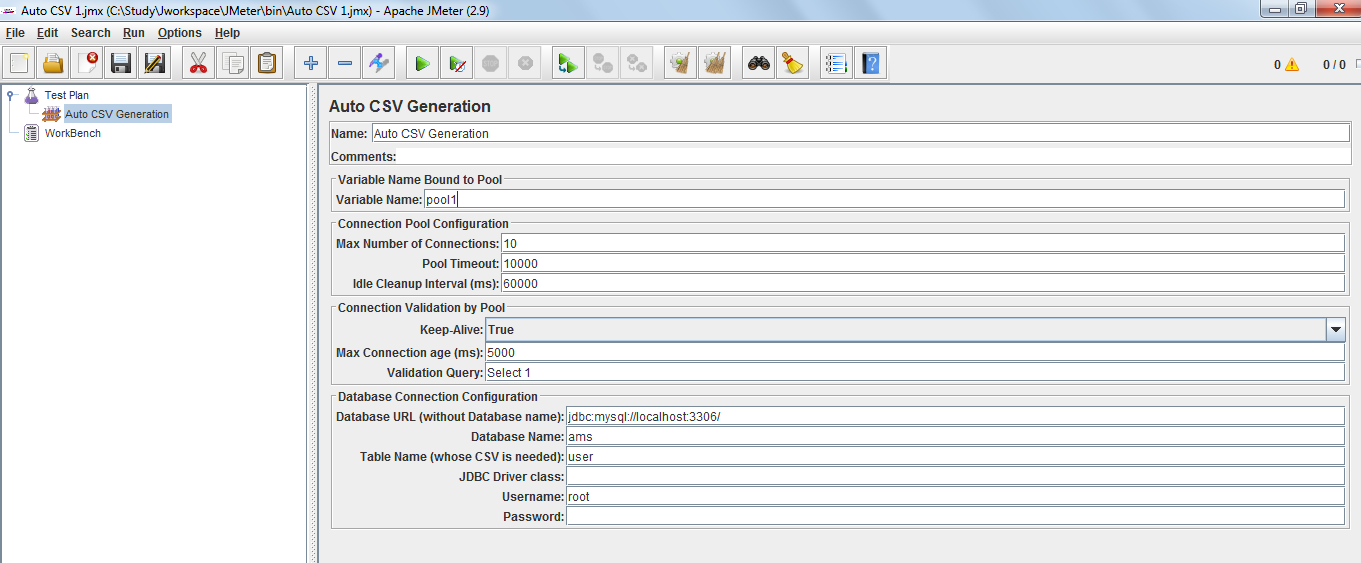
\includegraphics[width=14cm, height=8cm]{images/autocsvgeneration_1}
   \caption{Auto CSV Generation GUI\label{fig:fig15_JMeter}}
  \end{figure}
 
  \begin{itemize}
  \item \textbf{Name}: The name that tester wishes to give to the element. It will be displayed on the “Test Plan Tree”
  \item \textbf{Variable name}: Name of that JMeter variable to which the connection pool will be bound to. It is the data source pool. 
  \item \textbf{Max Number of Connections}: The maximum number of connections the pool will open at one time. By default it is set to 10.
  \item \textbf{Timeout}: After this time period the pool blocks request for connection, until new connections are available. This is the 
   maximum blocking time, until an exception is returned. It is in milliseconds. By default it is set to 10000ms (10sec).
  \item \textbf{Idle Cleanup Interval}: The pool removes extra idle connections at regular interval. This timing for interval is defined here.
    It is in milliseconds. By default it is set to 60000ms (60sec).
  \item \textbf{Keep Alive}: Whether the pool should validate connections. If no then the Connection Age and Validation Query are ignored.
  \item \textbf{Max Connection Age}: It is the maximum number of milliseconds an idle connection is kept, before discarding. It is in milliseconds.
    By default it is set to 5000ms
  \item \textbf{Validation Query}: A query used to validate if the connection is still alive. Relevant only if “Keep Alive” is true.
  \item \textbf{Database URL}: Full URL of the Database, including the JDBC protocol part, but excluding the database name only. The front slash “/” 
  before the database name should be present.
  \item \textbf{Database Name}: The name of the database for which the .csv file of one of the table is to be created.
  \item \textbf{Table Name}: The name of the table of database for which the .csv file will be created.
  \item \textbf{JDBC Driver class}: Full package and class name of the JDBC Driver to be used. It must be included in the JMeter class path beforehand. 
  \item \textbf{Username}: Username to use while connecting to database.
  \item \textbf{Password}: Password to use while connecting to database.
 \end{itemize}
 
 \section{Filtered Results Listener Plugin}
 The GUI for Filtered Results Listener Plugin is quite simple; user can select the appropriate operator, specify the value and run the test.
 
  \begin{figure}[H]
   \centering
   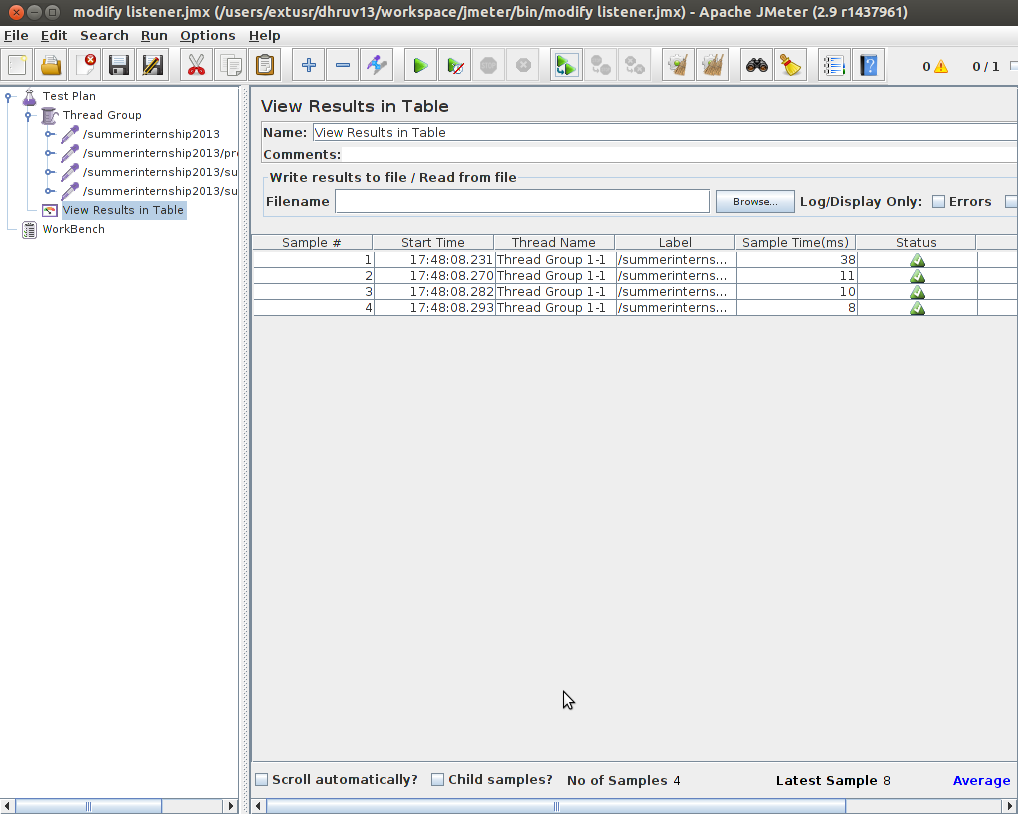
\includegraphics[width=14cm, height=8cm]{images/filteredresults_1}
   \caption{Old GUI without filtered results in ``View Results in a Table''\label{fig:fig16_JMeter}}
  \end{figure}
  
  \begin{figure}[H]
   \centering
   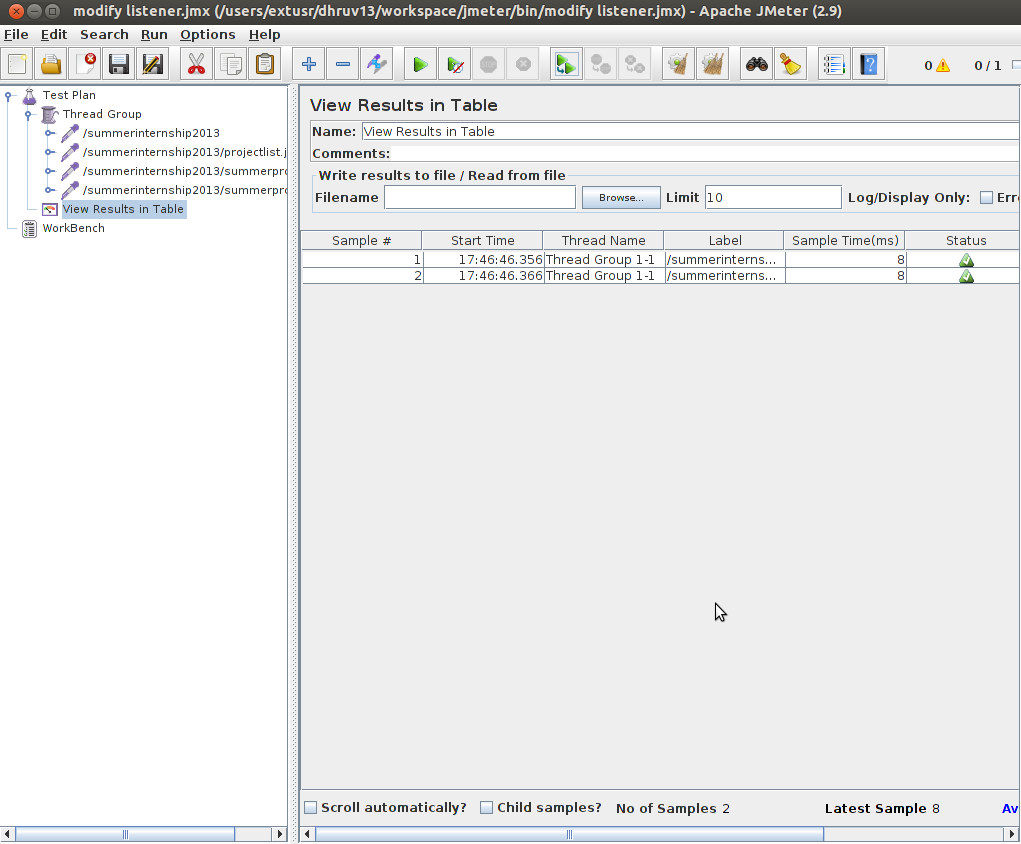
\includegraphics[width=14cm, height=8cm]{images/filteredresults_2}
   \caption{New GUI with filter \textbf{'Limit'} in ``View Results in a Table''\label{fig:fig17_JMeter}}
  \end{figure}
  
 \section{SMTP Defaults GUI}
 The graphical user interface for the SMTP defaults consist fields for the users to provide the
defaults values to be set in the test plan. They are name of the component, comments, server
name or address, port number or address, mail address to.

  \begin{figure}[H]
   \centering
   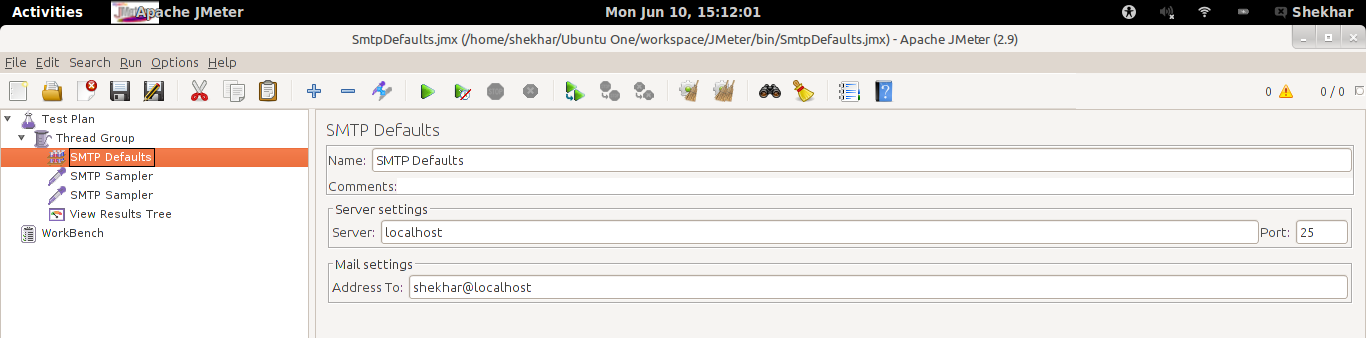
\includegraphics[width=14.5cm, height=6cm]{images/smtpdefaults_1}
   \caption{SMTP Defaults Config GUI\label{fig:fig18_JMeter}}
  \end{figure}

  Fields in SMTP defaults GUI:
  \begin{itemize}
   \item \textbf{Name}: Name of the config element in the test plan. This name is used to identify the element in the tree view of the test plan
   \item \textbf{Comments}: This text field is provided to give some related comment or description of the element used in the test plan.
   It may describe the use of the element in the test plan.
   \item \textbf{Server Settings Panel}
    \subitem \textbf{Server}: This text field is used specify the IP address or the domain name of the mail server where all the mails under this 
    config element is to be sent. This value is used by all the smtp samplers with in this config element in the hierarchy unless a sampler has 
    specifically specified the value for server.
    \subitem \textbf{Port}: This text field is used to specify the port address on which the mails are to be sent. 
   \item \textbf{Mail Settings Panel}
    \subitem \textbf{Address To}: This text field is used to specify the mail address where all the mails from the samplers in the test plan
    hierarchy will be delivered. Once specified, this value is used by all the samplers in the hierarchy unless a sampler has specifically specified
    the value for address to.
  \end{itemize}
  
  Once specified, all the samplers in the test plan will use the same port address unless a sampler has specifically specified the value for port.
  
  \section{GUI for TPC-C Sampler}
  
  The TPCC Sampler GUI  class generates the required GUI for the TPCC sampler. The code is based on Java awt and swings as are the other GUI classes of JMeter.


  \begin{figure}[H]
   \centering
   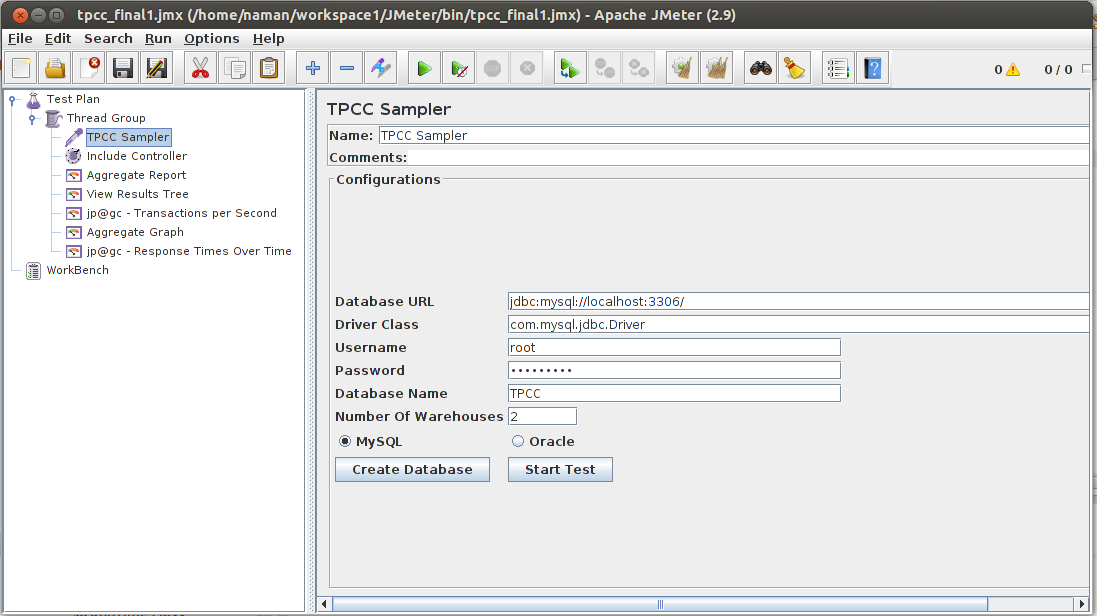
\includegraphics[width=15cm, height=7cm]{images/tpcc_71}
   \caption{TPC-C Sampler GUI\label{fig:fig64_JMeter}}
  \end{figure}
  
  The above figure shows the GUI for the sampler being generated. It takes as parameters Database URL, Driver class, Username , password , name of the database 
  to be created and the number of warehouses to be generated. Also a radio button is added, to specify if the database is MySQL or Oracle. Currently the TPC-C test
  supports only  these two databases.\\
  When the user  clicks the ‘’create database’’ button depending on the number of warehouses generated the 9 tables mentioned in the database schema and the 5
  procedures mentioned above get generated automatically and the tables also get filled with the required amount of data corresponding to the number of warehouses,
  using random values as specified in the TPC-C specifications.\\
  Similarly when the user clicks on the “start test” button the procedures which are generated in the database are called with parameters being random numbers and 
  strings generated by the 15 functions added by us in the JMeter source code.\\

  
  
  \section{Bandwidth Throttling GUI}
  Bandwidth throttling element have been added with in the HTTP Request Defaults 'config
element' of JMeter. It mainly consists of two components apart from the components which are
already there in the config element. They are 'Use bandwidth Throttling' check box and
Bandwidth (in cps) text box.

  \begin{figure}[H]
   \centering
   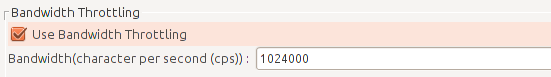
\includegraphics[width=10cm, height=2cm]{images/bandwidth_1}
   \caption{Bandwidth Throttling element in Http Requests Defaults\label{fig:fig19_JMeter}}
  \end{figure}
  
Field elements in the GUI:
 \begin{itemize}
  \item \textbf{Use Bandwidth Throttling}: A check box which enables bandwidth throttling in JMeter. When this check box is selected,
  the text box for the bandwidth is enabled.
  \item \textbf{Bandwidth (Character per second)}: This is a text box enabled only when bandwidth throttling check box is selected. 
  The value specified in this check box is used by the JMeter as the bandwidth available for the System.
 \end{itemize}
 
\section{Dynamic Bandwidth Throttling GUI}
Dynamic Bandwidth throttling element has been added with in the HTTP Request Defaults
'config element' of JMeter. It mainly consists of three components apart from the components
which are already there in the config element.

  \begin{figure}[H]
   \centering
   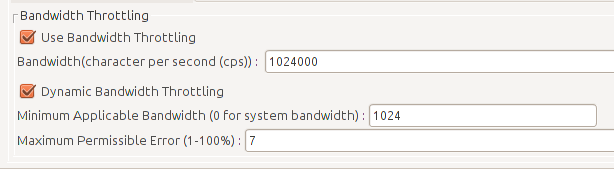
\includegraphics[width=14cm, height=4cm]{images/dbandwidth_1}
   \caption{Dynamic Bandwidth Throttling GUI\label{fig:fig20_JMeter}}
  \end{figure}
  
Fields in the Dynamic Bandwidth Throttling GUI component:
  \begin{itemize}
   \item \textbf{'Dynamic Bandwidth Throttling' Check Box} : This check box is used to set the use of dynamic bandwidth with JMeter. Once selected, 
   this enables the use of dyanmic bandwidth variations. Enabling this component also enable the text fields in the GUI.
   \item \textbf{Minimum Applicable Bandwidth} : This sets the minimum level for the bandwidth upto which the bandwidth can be reduced during runtime. 
   Default value is 0.
   \item \textbf{Maximum Permissible Error}: This text box is used to specify the threshold value which will be used to vary the bandwidth. If the error crosses this value, 
      then the bandwidth starts decreasing until the error again gets below this value or reaches the minimum applicable bandwidth value specified in the previous 
      text field. Default is 100\%.
  \end{itemize}
  
\section{IP Spoofing Config Element GUI}

  \begin{figure}[H]
   \centering
   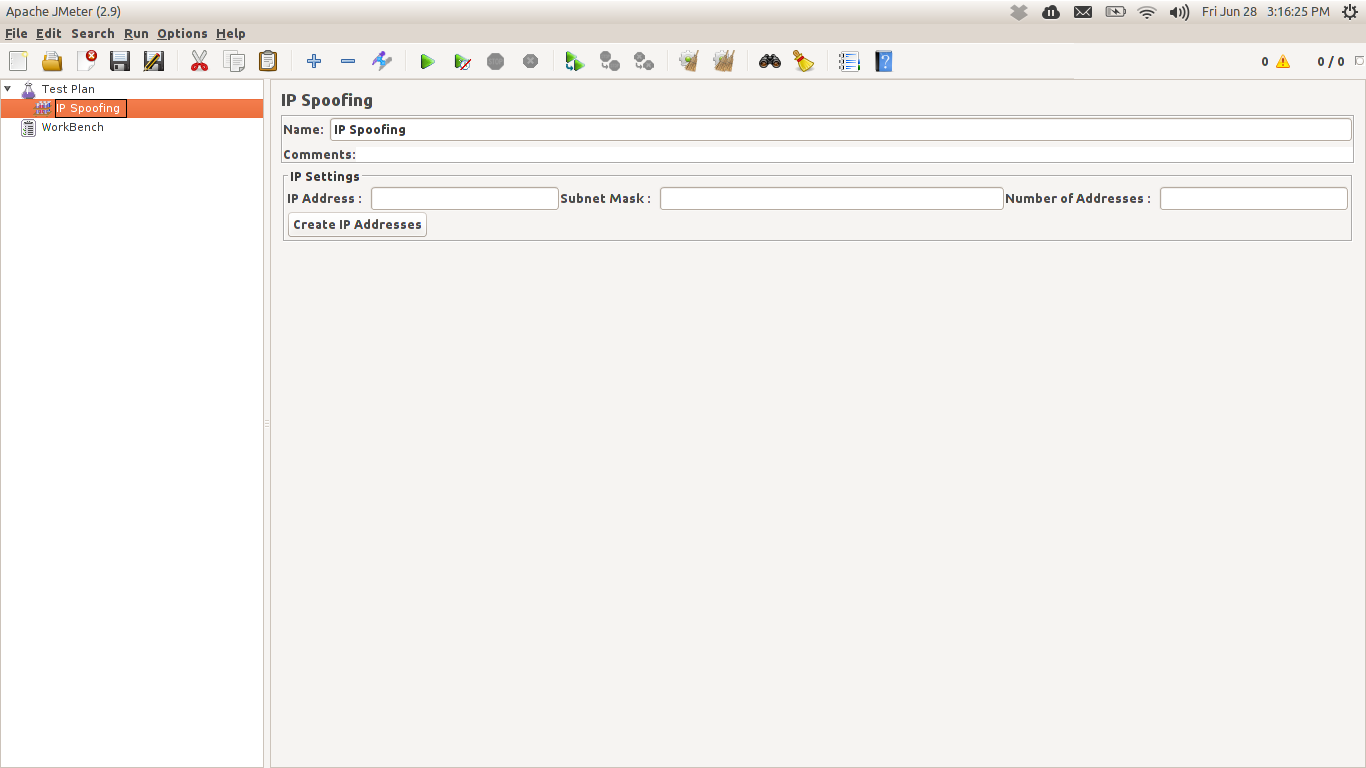
\includegraphics[width=14cm, height=4cm]{images/ip_71}
   \caption{IP Spoofing Config Element GUI\label{fig:fig83_JMeter}}
  \end{figure}
  
  \textbf{GUI Components}
  \begin{itemize}
   \item \textbf{IP address}: The starting IP’s of the subnet from where the alias IP addresses are to be added in the system
   \item \textbf{Subnet Mask}: Subnet mask of the IP’s to be added.
   \item \textbf{Number of addresses} : The number of IP’s to be generated and to be added to the system.
   \item \textbf{Create IP addresses} : Clicking this button creates the IP’s, starting from the given IP address.
  \end{itemize}


  
\chapter{Demonstrations of Test Plans}
  \section{Demonstration of ``Auto CSV Generation'' config element}
  
  \textbf{Aim}: The aim of running this test is to automatically create the .csv file for the table of database
      mentioned, using ``Auto CSV Generation'' and to use it along with samplers to supply data to
      samples under use in test.\\
      \\
  \textbf{Procedure}: The main purpose of the ``Auto CSV Generation'' is to create .csv file and have it in
      the ``bin'' folder of JMeter to be used by other samplers.

  
  \begin{figure}[H]
   \centering
   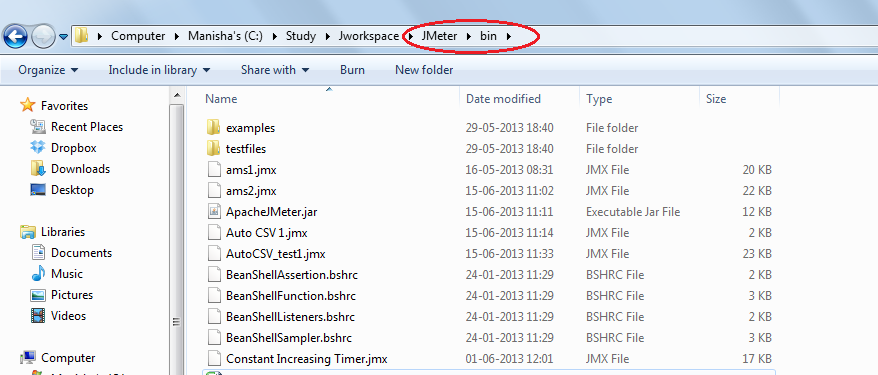
\includegraphics[width=15cm, height=8cm]{images/autocsvgeneration_81}
   \caption{'bin' directory before CSV file generation\label{fig:fig21_JMeter}}
  \end{figure}
  
  The database name and table name, along with connection details, is mentioned in the interface,
  and the new csv file will be named as databaseName\_tableName.csv, and can be found in the bin
  of JMeter.\\
  
  \begin{figure}[H]
   \centering
   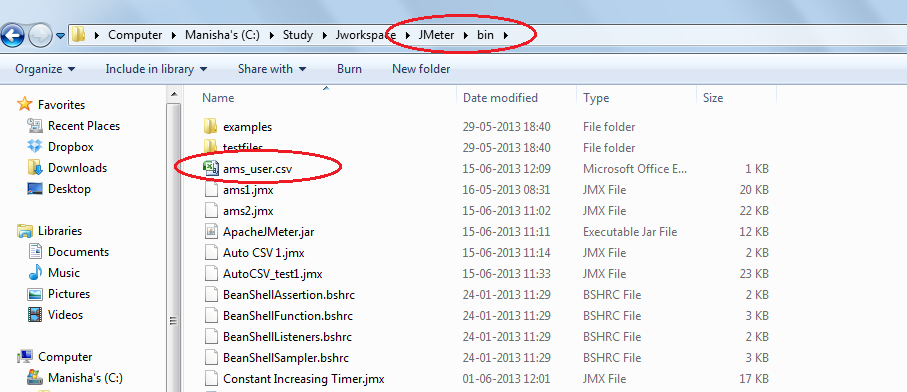
\includegraphics[width=15cm, height=8cm]{images/autocsvgeneration_82}
   \caption{'bin' directory after CSV file generation\label{fig:fig22_JMeter}}
  \end{figure}
  
  The .csv file, created during a JMeter experiment with Database –ams and Table –user, has the
  following content.
  
  \begin{figure}[H]
   \centering
   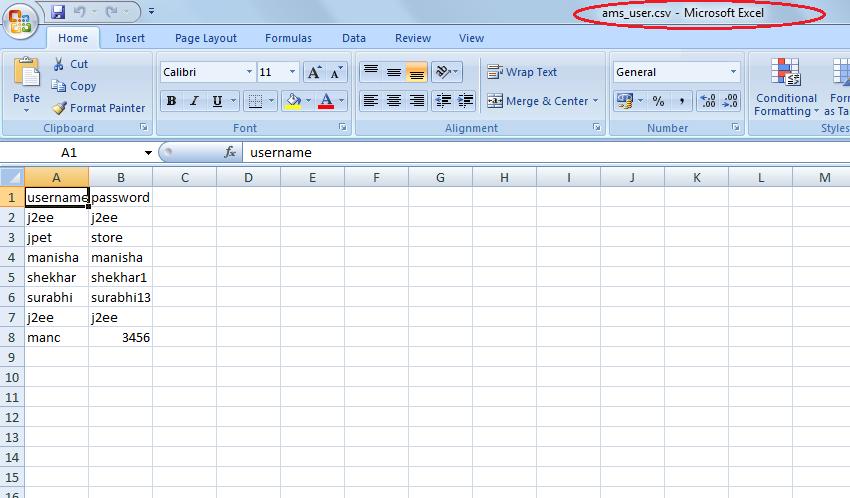
\includegraphics[width=15cm, height=8cm]{images/autocsvgeneration_83}
   \caption{The ams-user.csv file in MS Excel\label{fig:fig23_JMeter}}
  \end{figure}  
  
  The application under test (AUT) is a simple web-app, for airport management people, the
  opening page of which expects user name and password as user (manager) input, checks against
  Database already present and then creates session for users. Thus here the parameters passed are
  username and password, which need to be unique for all user logged in simultaneously. For a
  web-server testing, with load of 100 or 1000 users, a csv file needs to be produced with 100 or
  1000 entries, for the login validation page. This job, when manually done, becomes hectic. But
  the new config element facilitates this generation automatically from the database specified.\\
  
  As we can see above, this csv file has already been created. Now this csv file needs to be
  clubbed with sampler, for its data to be used by sampler. The test plan below depicts it.
  
  \begin{figure}[H]
   \centering
   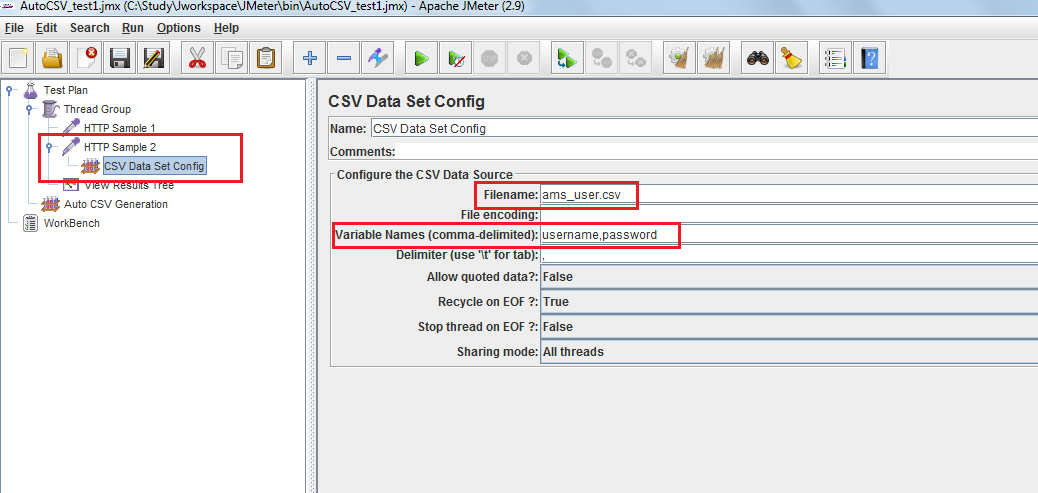
\includegraphics[width=15cm, height=7cm]{images/autocsvgeneration_84}
   \caption{Test plan with HTTP Samplers, to which “CSV data config” element is added as child\label{fig:fig24_JMeter}}
  \end{figure}    
  
  The ``CSV Data Set Config'' Configuration Element is a configuration element already present in
  JMeter. In the above view, the comma separated variables are those variables whose values are
  picked up from the .csv file. These variables are also defined in the HTTP sampler which takes
  the ``CSV Data Set Config'' as child.
  
  \begin{figure}[H]
   \centering
   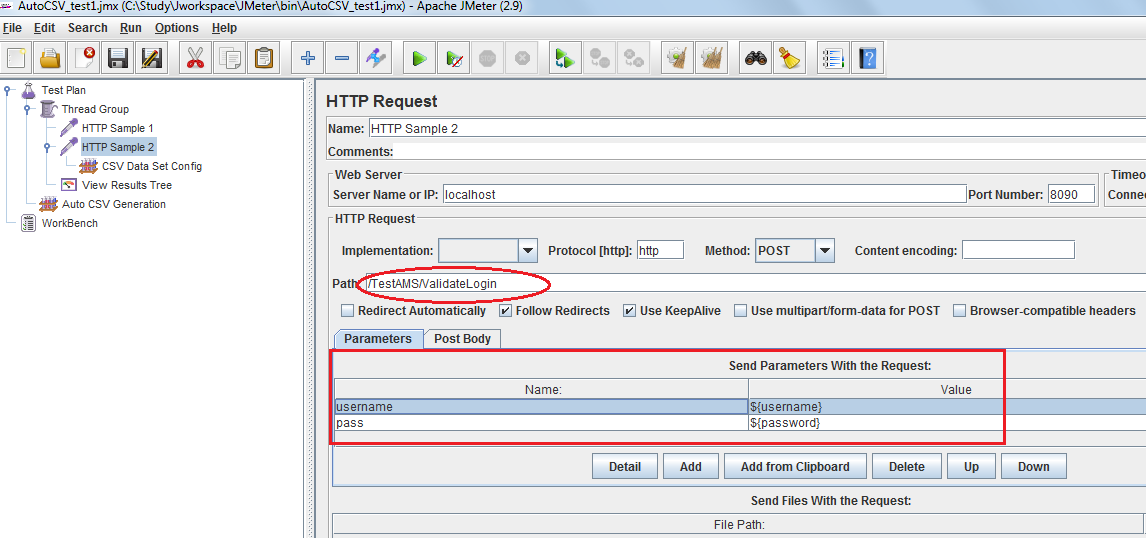
\includegraphics[width=15cm, height=7cm]{images/autocsvgeneration_85}
   \caption{The HTTP sampler, to which the .csv file is added as child\label{fig:fig25_JMeter}}
  \end{figure}    

  Here the parameters of request are set with variables mentioned in the ``CSV Data Set Config''.
  Then the test plan is played. The output of test is observed and it is seen that every request passes
  one set of values from .csv file as POST data, when ever that sample is used as user request.\\
  \\
  \textbf{Observation}
  
  \begin{figure}[H]
   \centering
   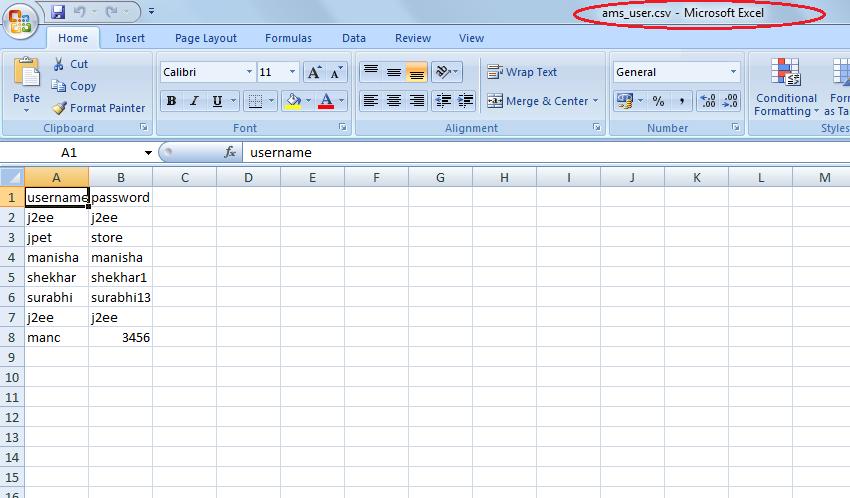
\includegraphics[width=15cm, height=8cm]{images/autocsvgeneration_86}
   \caption{Observation 1\label{fig:fig26_JMeter}}
  \end{figure}   
  
  \begin{figure}[H]
   \centering
   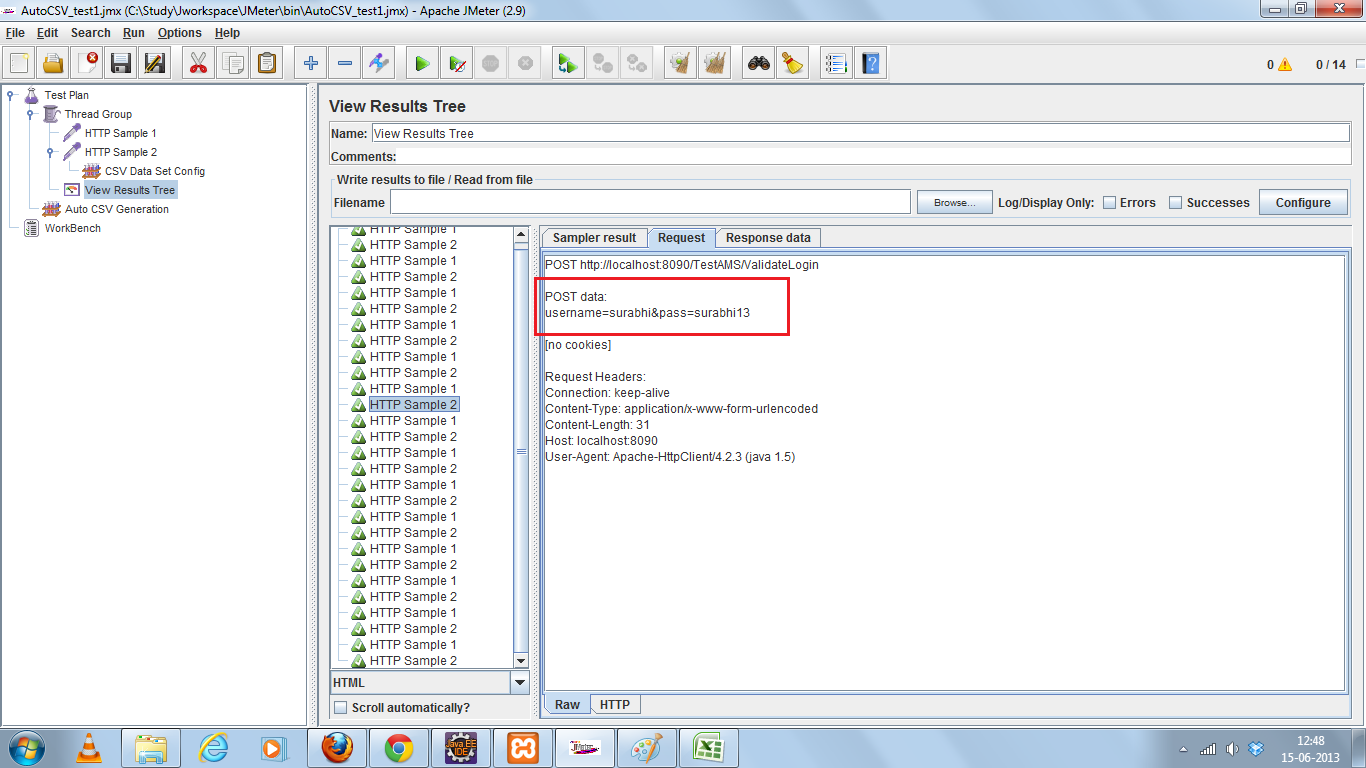
\includegraphics[width=15cm, height=8cm]{images/autocsvgeneration_87}
   \caption{Observation 2\label{fig:fig27_JMeter}}
  \end{figure}   
  
  \textbf{Conclusion}:
  Different requests take different set of data, successively from .csv file, and if the number of
  users is greater than the sets of data in the file, then the set of data are picked from the start of the
  file again. Thus the purpose of developing the new Auto CSV generation Config element was
  successful.
  
  \section{Demonstration of SMTP Defaults Config Element}
  
  \textbf{Aim}: A test plan to demonstrate the working of SMTP defaults in Apache JMeter.\\
  \\
  \textbf{System Requirements}: Apache JMeter 2.9 and Postfix and Dovecot Mail server need to be installed
      on the system to be used for testing.\\
  \\
  \textbf{Procedure}: The process to create the required test plan is described below\\
  \begin{itemize}
    \item Step 1: A thread group is added to test plan from Edit menu.\\
    \item Step 2: Number of threads is set to 1 and Loop count is set to 1. \textbf{See fig. 8.8}\\ 
    \item Step 3: An 'SMTP defaults' config element is added to thread group\\
    \item Step 4: Name of the element is left unchanged. In the server settings panel the server text box is
	    set to localhost, and port number is set to 25. In the mail settings panel Address is set
	    'shekhar@localhost' which is an email address configured on localhost mail server.
	    \textbf{See fig. 8.9}\\
    \item Step 5: An SMTP sampler is added from Edit menu. 'Address
	    from' field can be set to any value. Here it is set to 'shekharsaurav@localserver.com'.
	    The address format should be correct.\\
    \item Step 6: In the message settings of the sampler. The subject of the message is set to 'Subject of the
	    mail' and message text field is set to 'message of the mail'.
	    \textbf{See fig 8.10}\\
    \item Step 7: Another SMTP Sampler is added to the thread group and in the message setting panel, the
	    value for subject is set to 'Subject for the mail 2' and message is set to 'message for the
	    mail 2'. \textbf{See fig 8.11}\\
    \item Step 8: A 'View Results Tree' listener is added to the thread group from Edit Menu.\\
  \end{itemize}
  
    
  \begin{figure}[H]
   \centering
   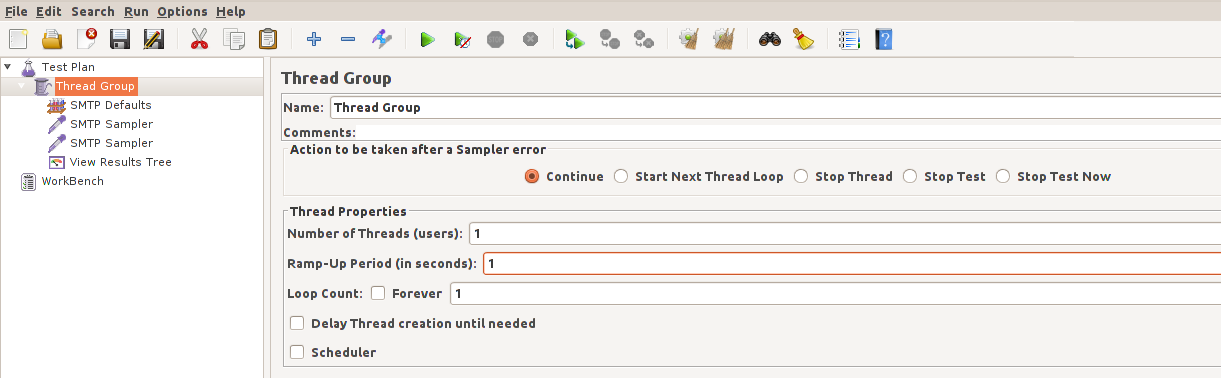
\includegraphics[width=15cm, height=5cm]{images/smtpdefaults_81}
   \caption{Thread group in the test plan\label{fig:fig28_JMeter}}
  \end{figure} 
  
  \begin{figure}[H]
   \centering
   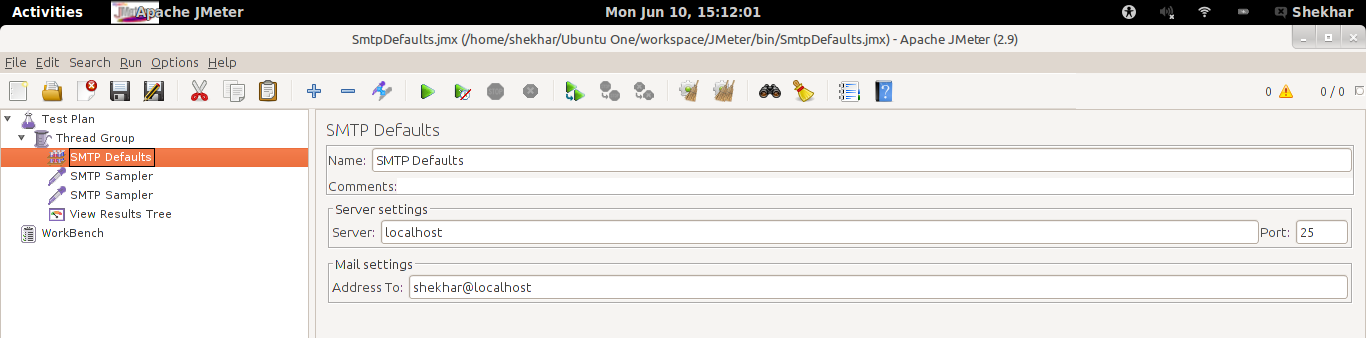
\includegraphics[width=15cm, height=5cm]{images/smtpdefaults_82}
   \caption{SMTP Defaults in the test plan\label{fig:fig29_JMeter}}
  \end{figure}   
  
  \begin{figure}[H]
   \centering
   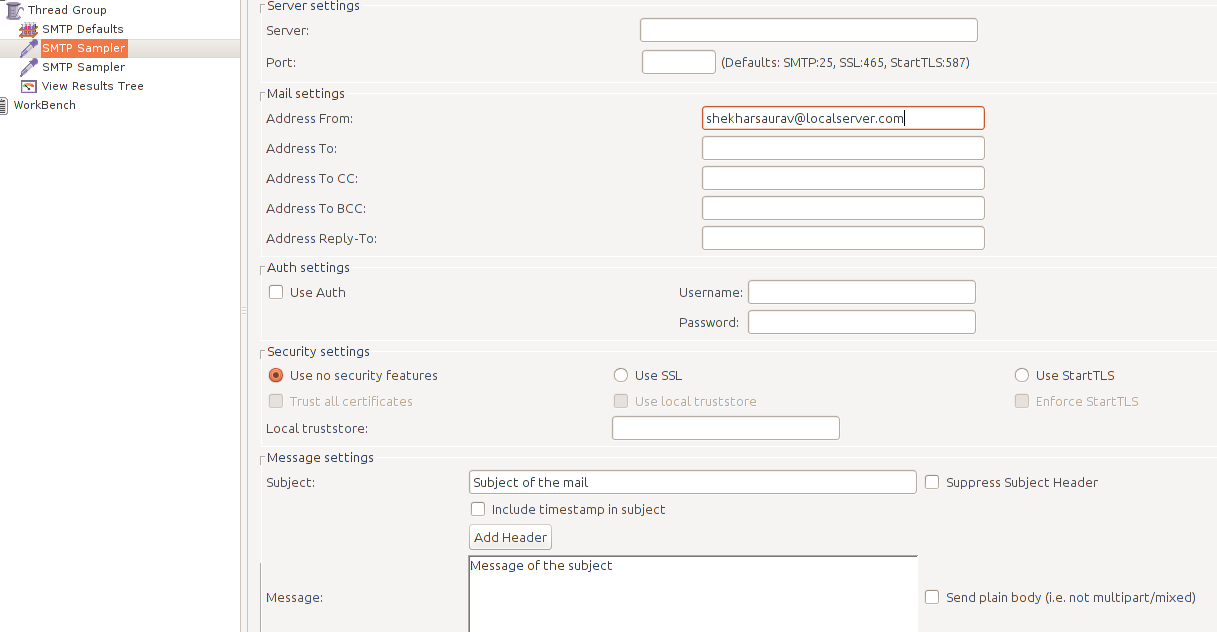
\includegraphics[width=15cm, height=8cm]{images/smtpdefaults_83}
   \caption{First SMTP sampler in the test plan\label{fig:fig30_JMeter}}
  \end{figure} 
  
  \begin{figure}[H]
   \centering
   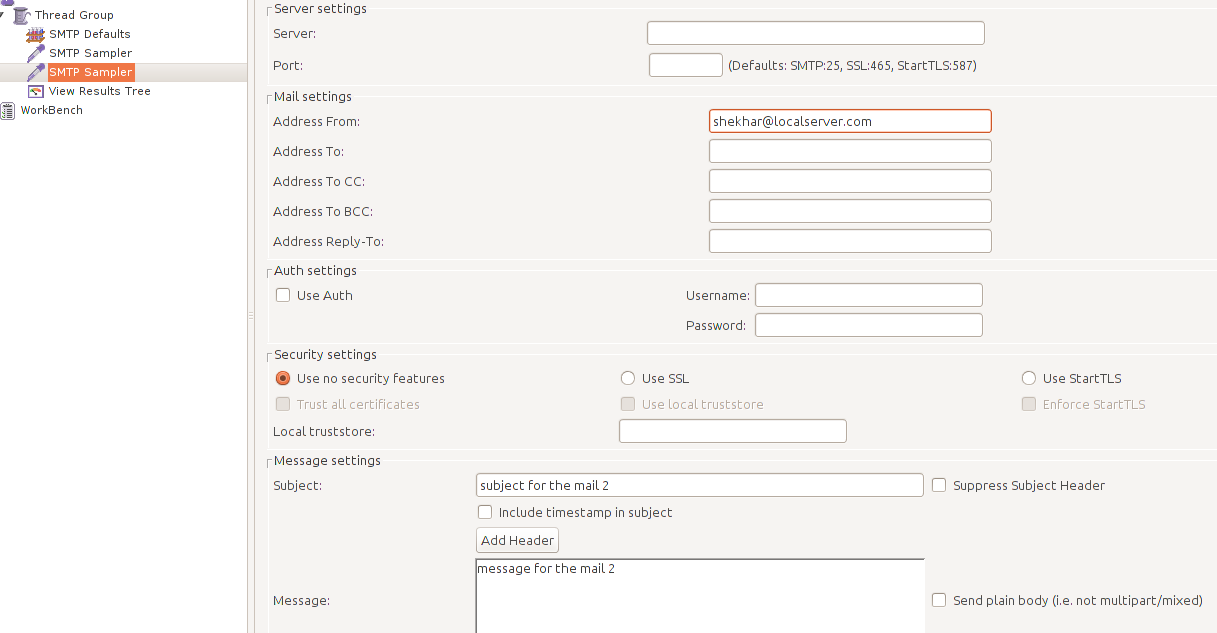
\includegraphics[width=15cm, height=8cm]{images/smtpdefaults_84}
   \caption{Second SMTP sampler in the test plan\label{fig:fig31_JMeter}}
  \end{figure} 
  
  Now the Test Plan is ready to be executed. The test plan is run and the results are recorded.\\
  \\
  \textbf{Observation}:
  \\
  Results for first sampler:\\
  \begin{figure}[H]
   \centering
   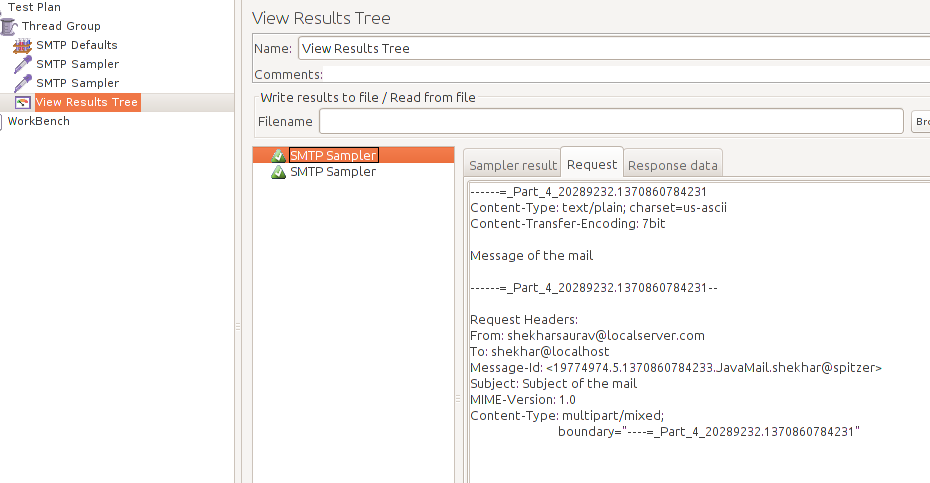
\includegraphics[width=15cm, height=8cm]{images/smtpdefaults_85}
   \caption{Results Tree Listener for first sampler in the test plan after the test completion\label{fig:fig32_JMeter}}
  \end{figure}
  
  Fig 8.12 shows the result tree for the first sampler. The request shows the message of the mail
  sent and the green icon besides the SMTP sampler shows the successful delivery of the message.
  The figure 8.13 shows the mail inbox showing the mail received from the first sampler.
  
  \begin{figure}[H]
   \centering
   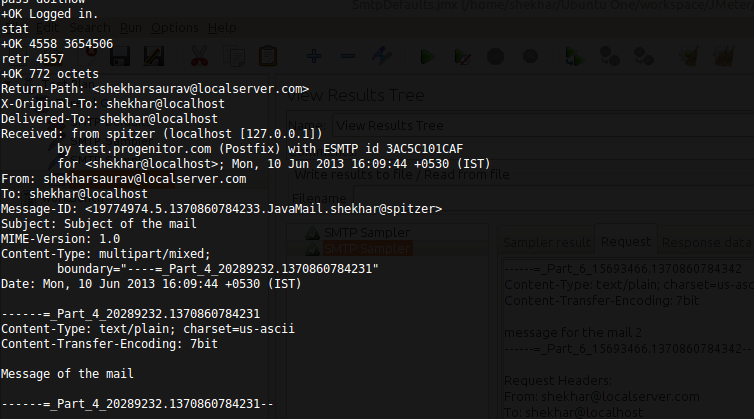
\includegraphics[width=15cm, height=8cm]{images/smtpdefaults_86}
   \caption{Mail inbox showing the recieved message from first sampler\label{fig:fig33_JMeter}}
  \end{figure}
  
  Results for second sampler:\\
  
  \begin{figure}[H]
   \centering
   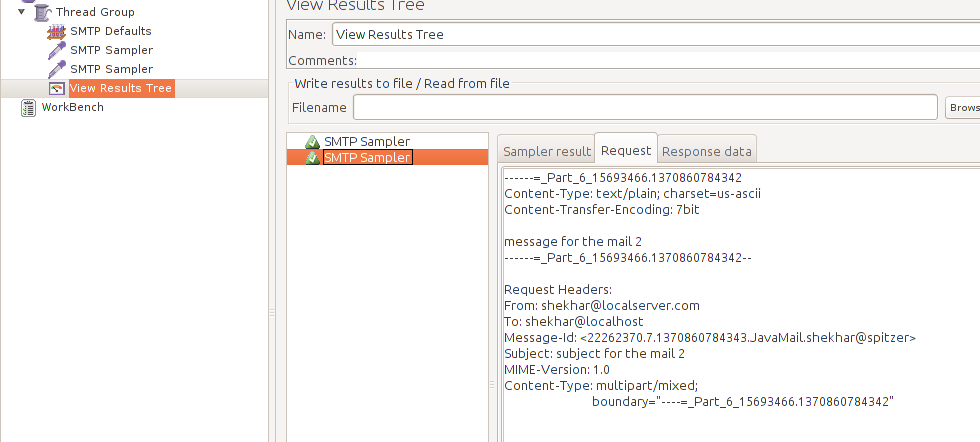
\includegraphics[width=15cm, height=8cm]{images/smtpdefaults_87}
   \caption{Results Tree Listener for second sampler in the test plan after the test completion\label{fig:fig34_JMeter}}
  \end{figure}
  
  
  Fig 8.14 shows the result tree for the second sampler. The request shows the message of the mail
  sent and the green icon besides the SMTP sampler shows the successful delivery of the message.
  The figure 8.15 shows the mail inbox showing the mail received from the second sampler.
  
  \begin{figure}[H]
   \centering
   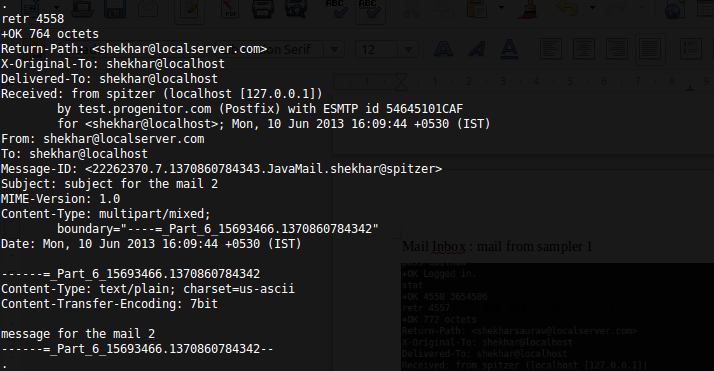
\includegraphics[width=15cm, height=6cm]{images/smtpdefaults_88}
   \caption{Mail inbox showing the recieved message from second sampler\label{fig:fig35_JMeter}}
  \end{figure}
  
  \textbf{Conclusion}:
  After the completion of the test we verified the results by checking the mails recieved in the mail server as shown in the figures above.
  This test varified the proper working of SMTP Defaults config element.
  
 \section{Automatic TPC-C testing in JMeter}
  We have automated the lengthy process of TPC-C testing, making JMeter capable of carrying out a basic preliminary TPC-C test.
  The process followed by TPC-C has been emulated in a test script firing the exact transactions and taking the exact parameters as 
  defined by TPC-C standards.\\
  Currently, we have automated TPC-C testing only for MySQL and Oracle database.\\
  Steps for carrying out the tpcc test in JMeter:
 \begin{enumerate}
  \item Open JMeter.
  \item Include the test scripts tpcc\_test\_mysql.jmx, tpcc\_test\_oracle.jmx, tpcc\_test.jmx into the bin folder of JMeter.
  \item Open a new test plan. 
  \item First add a thread group to the test plan.\\
	Test Plan \textgreater Add \textgreater Threads \textgreater Thread Group 
  \item Enter the number of users for the test, in the “No of Threads” field of the GUI of Thread Group. 
  \item Provide a Ramp-up time for the test, if required.
  \item Add a TPCC Sampler into the test plan.\cite{Results}\\ 
        Thread Group \textgreater Add \textgreater Sampler \textgreater TPCC Sampler
  \item Add an Include Controller into the test plan.\\
        Thread Group \textgreater Add \textgreater Logic Controller \textgreater Include Controller.
  \item	If you want to test an oracle database, browse into the bin directory of JMeter and include the test plan named tpcc\_test\_oracle.jmx, 
	else if you want to test for a MySQL database include tpcc\_test\_mysql.jmx.
  \item Add Listeners to the test plan,\\
	Thread Group \textgreater Add \textgreater Listener \textgreater Aggregate Report\\ 
	Thread Group \textgreater Add \textgreater Listener \textgreater View Results Tree\\
	Thread Group \textgreater Add \textgreater Listener \textgreater Aggregate Graph\\
	Add Transactions per Second and Response Time over times Listener for better visualization.\\
  \item Click on the TPCC Sampler. 
  \item The TPCC Sampler GUI is displayed.
  \item Enter the required information to establish connection. In the url field, give the url excluding the database name. eg.jdbc:mysql://localhost:3306/
  \item Enter the database name in the database field.
  \item Enter the number of warehouses.
  \item Click on Create Database Button to create the database and populate it.
  \item Click on Start test Button to start the test. \\
	\textbf{Note}- Do not press run on jmeter toolbar, click start test in the GUI of the TPCC Sampler.
  \item In the aggregate report Listener, the noted throughput of the New Order Transaction is the required Performance metric for TPC-C test, tpm-C, 
	the number of new order transactions per minute.
 \end{enumerate}
 
  \textbf{Note}: If you are doing an oracle testing ,kindly update your default accepted date format to ‘dd-MMM-yy’
  Initially we tested the database by creating one warehouse. Here are the observations of the experiment.\\
  
  \begin{figure}[H]
    \centering
    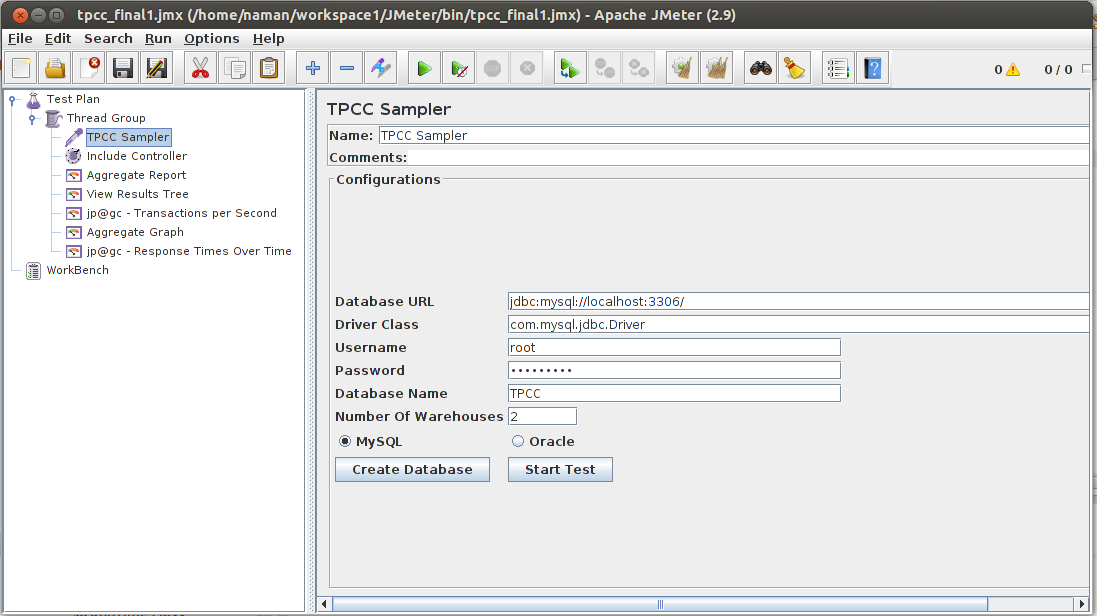
\includegraphics[width=15cm, height=8cm]{images/ntpcc_81}
    \caption{Test plan for TPC-C preliminary test\label{fig:fig65_JMeter}}
  \end{figure} 
   
  This is the test plan taken for performing TPC-C preliminary test. We have explained the test conducted for MySQL database.\\
  The test plan includes an Include Controller which includes the actual TPC-C test script.
  
  \begin{figure}[H]
    \centering
    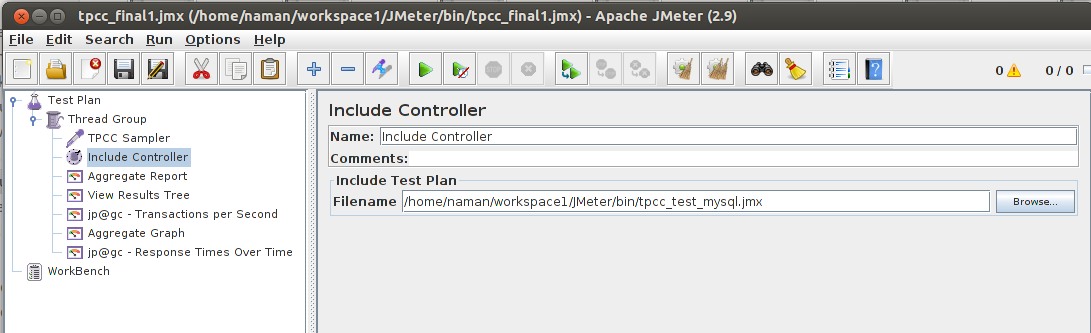
\includegraphics[width=15cm, height=6cm]{images/ntpcc_82}
    \caption{Include Controller for including the actual TPC-C test script\label{fig:fig66_JMeter}}
  \end{figure} 
   
   First, the no of warehouse is given as 1, and the create database clicked.\\
  As is clearly visible from the images shown below, the required tables and procedures with the required data get generated in the database. The general measure
  is that for 1 warehouse about 120MB of data is generated in the user’s database, which gets multiplied depending on the number of databases. \\

  \begin{figure}[H]
    \centering
    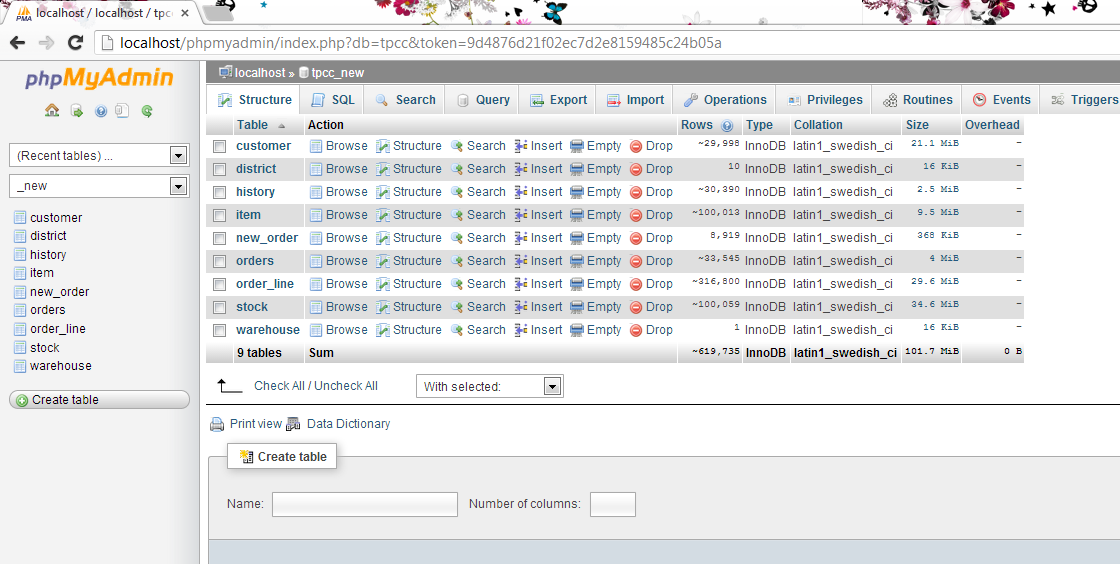
\includegraphics[width=15cm, height=8cm]{images/ntpcc_83}
    \caption{Tables generated in the database for Case 1: 1 warehouse\label{fig:fig67_JMeter}}
  \end{figure} 
  
  \begin{figure}[H]
    \centering
    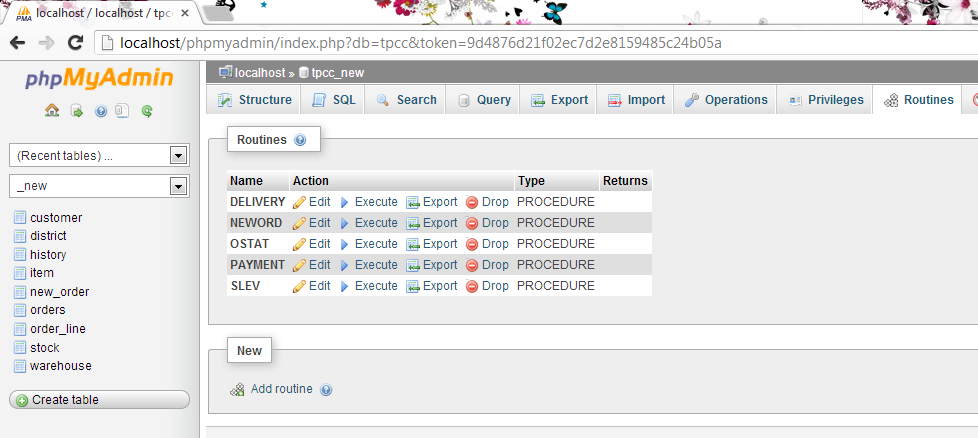
\includegraphics[width=15cm, height=8cm]{images/ntpcc_84}
    \caption{List of routines generated in the database.\label{fig:fig68_JMeter}}
  \end{figure} 
  
  Similarly we extended the test carrying out an experiment with the creation of 33 warehouses. The following results were observed:
  
    
  \begin{figure}[H]
    \centering
    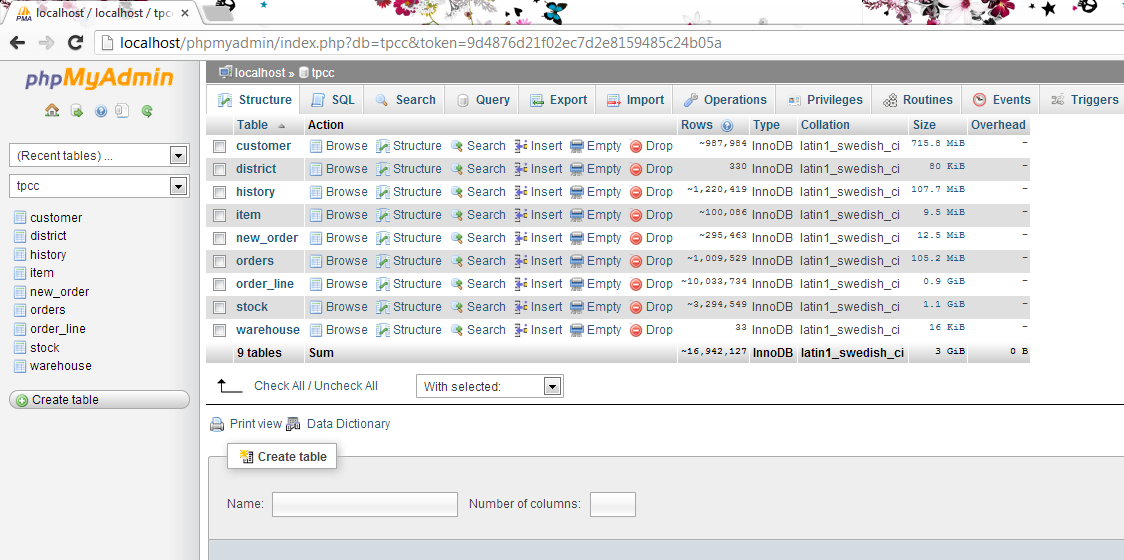
\includegraphics[width=15cm, height=8cm]{images/ntpcc_85}
    \caption{Tables generated in the database for Case 2: 33 warehouses\label{fig:fig69_JMeter}}
  \end{figure} 
  
  As can be seen, all the tables have been created successfully with the expected amount of data.
  All the five procedures have also been added to the database.\\
  JMeter being a server load testing tool can be used in carrying out preliminary TPC-C testing. JMeter can create emulated users as the number of threads in it, 
  send transaction requests to the server, and get the response.\\
  \\The procedure of the benchmarking tests includes steps which can as well be automated in JMeter. \\


  A manual test script created in JMeter for TPC-C testing follows.\\

  In the thread group component, the no of virtual users, the ramp up period can be set up and scheduling of the test can be done. \\
  
  \begin{figure}[H]
    \centering
    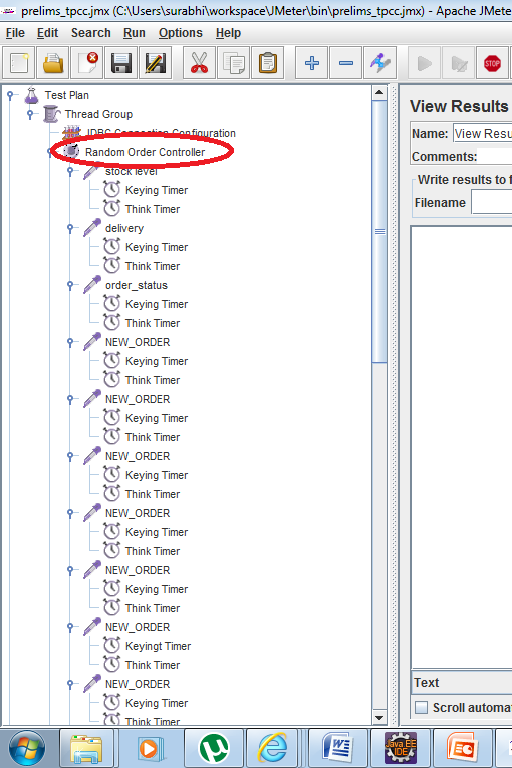
\includegraphics[width=7cm, height=10cm]{images/ntpcc_86}
    \caption{23 samples are taken in the test plan. \label{fig:fig70_JMeter}}
  \end{figure} 

  \begin{itemize}
   \item 10 New\_order samplers. 
   \item 10 Payment samplers 
   \item 1 delivery sampler 
   \item 1 order\_status sampler. 
   \item 1 stock\_level sampler. 
  \end{itemize}

  A Random Order Controller has been included in the test plan. It will execute all the samples within it in a random order, making sure
  A  each sample is executed only once.\\
  
  \begin{figure}[H]
    \centering
    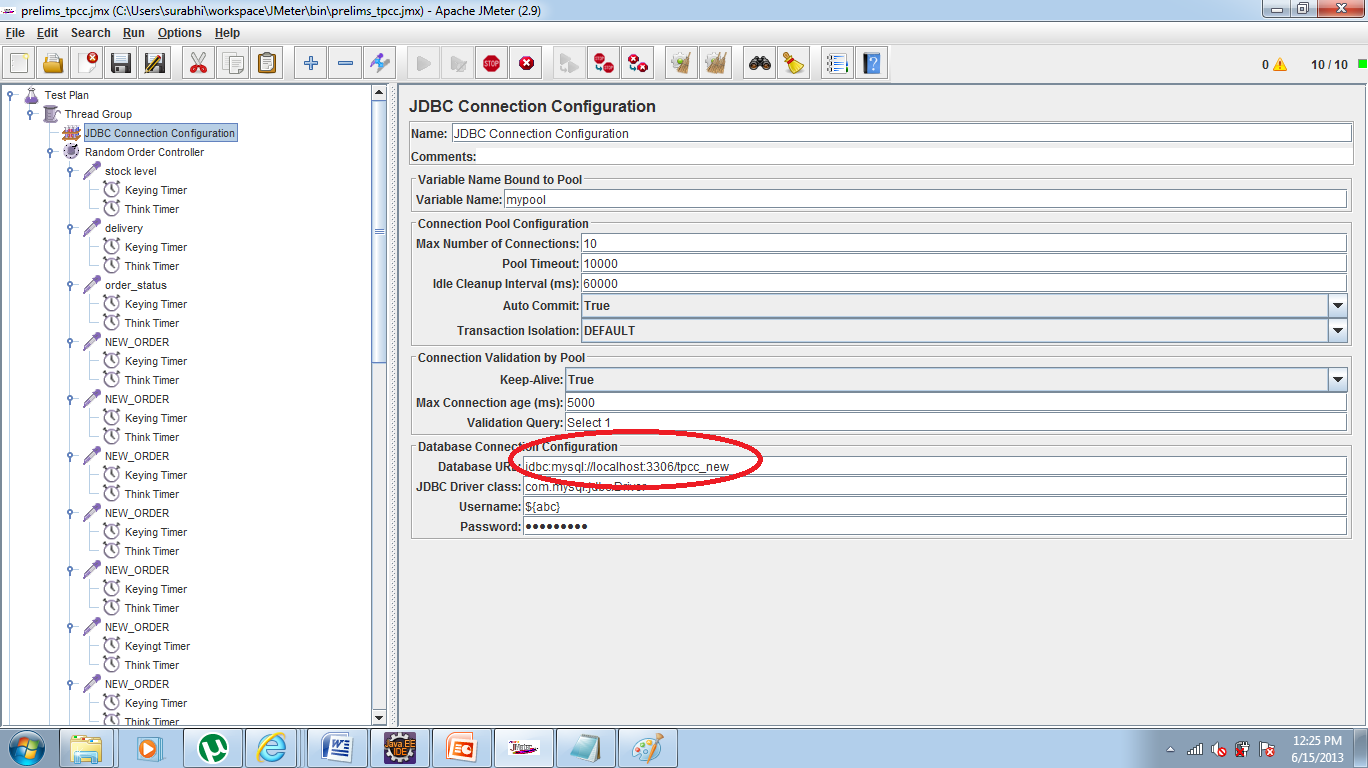
\includegraphics[width=15cm, height=8cm]{images/ntpcc_87}
    \caption{JDBC Connection Configuration for the test plan\label{fig:fig71_JMeter}}
  \end{figure} 
  
  In the JDBC Connection Configuration, the connection parameters are given. These parameters are internally passed from the TPC-C Sampler GUI to the 
  included test script via the Include Controller through functions created in JMeter.\\
  
  \begin{figure}[H]
    \centering
    \includegraphics[width=15cm, height=8cm]{images/ntpcc_88}
    \caption{Constant Timer for the test plan\label{fig:fig72_JMeter}}
  \end{figure} 

    As a child of each sampler, keying time and think time timers are included.
  The keying time emulates the time taken by the user to enter the parameters for a transaction.The Keying time is a constant timer for each transaction.
    The values are:
   
  \begin{table}[h]
   \begin{center}
    \begin{tabular}{|c|l|p{5cm}|} 
    \hline
    \textbf{Sl No.} & \textbf{Transaction Name} & \textbf{Keying Time}\\
    \hline
    1 & New Order & 18 sec \\
    \hline
    2 & Payment & 3 sec \\
    \hline
    3 & Delivery & 2 sec \\
    \hline
    4 & Order Status & 2 sec \\
    \hline
    5 & Stock level & 2 sec \\
    \hline    
    \end{tabular}
    \caption{Keying time for different transactions in TPC-C}
   \end{center}
  \end{table}
  
  The generation of parameters for calling each procedure also takes some time, so we have
  reduced 1 sec from each keying time and fed to the timer.
 
   \begin{figure}[H]
    \centering
    \includegraphics[width=15cm, height=8cm]{images/ntpcc_89}
    \caption{Think Timer for the test plan\label{fig:fig73_JMeter}}
   \end{figure} 
   
   The think time has a constant mean value. So, the Guassian Random Timer is used here. We
   specify the mean value think time for the transaction as the constant delay offset.
   The think time emulates the time taken by the user to select a transaction after the completion of one transaction.\\
   The mean think time for the transactions are:\\
   
  \begin{table}[h]
   \begin{center}
    \begin{tabular}{|c|l|p{5cm}|} 
    \hline
    \textbf{Sl No.} & \textbf{Transaction Name} & \textbf{Think Time}\\
    \hline
    1 & New Order & 12 sec \\
    \hline
    2 & Payment & 12 sec \\
   \hline
    3 & Delivery & 10 sec \\
    \hline
    4 & Order Status & 5 sec \\
    \hline
    5 & Stock level & 5 sec \\
    \hline    
    \end{tabular}
    \caption{Think time for different transactions in TPC-C}
   \end{center}
  \end{table}
  
   \begin{figure}[H]
    \centering
    \includegraphics[width=15cm, height=8cm]{images/ntpcc_90}
    \caption{JDBC Request sampler for Payment transaction for the test plan\label{fig:fig74_JMeter}}
   \end{figure}
   
   The above is a snapshot of one of the transactions- Payment.\\
   The transaction is called as a callable statement procedure from a jdbc sampler. The procedure
   takes 33 parameters. The IN parameters values are calculated from calling functions stored in
   JMeter. The functions required to be called have been created and stored in JMeter functions
   directory and as a result are listed in the Function Helper Tool of JMeter and can be selected from
   here also.
   
  \begin{figure}[H]
    \centering
    \includegraphics[width=15cm, height=8cm]{images/ntpcc_91}
    \caption{Functions added to Function Helper list\label{fig:fig75_JMeter}}
   \end{figure}
   
   Some functions shown,e.g. \_getItemID , \_getLastName, \_getNURandLNameRun,
   \_GetWarehouseID, etc. have been added to the list.\\
   A total of 15 new functions classes have been added here to get the required functionality needed to create the parameters to call the procedures.\\

   The test is run clicking on the Start test button in the GUI of the TPC-C Sampler.\\
   The results can be viewed in the Listeners added in the test plan.\\
    
  \begin{figure}[H]
    \centering
    \includegraphics[width=15cm, height=6cm]{images/ntpcc_92}
    \caption{View Results Tree Listener after the test run\label{fig:fig76_JMeter}}
   \end{figure}
   As can be seen in the request sent, all the functions have been resolved at runtime and the actual
   values are being sent.


   \begin{figure}[H]
    \centering
    \includegraphics[width=15cm, height=8cm]{images/ntpcc_93}
    \caption{Response Data in View Results Tree Listener showing OUT and INOUT parameters of the procedure\label{fig:fig77_JMeter}}
   \end{figure}
   

   The response data gives the values of all the OUT and INOUT parameters of the procedures.\\
   
  \begin{figure}[H]
    \centering
    \includegraphics[width=15cm, height=8cm]{images/ntpcc_94}
    \caption{Aggregate Report for the test plan\label{fig:fig78_JMeter}}
   \end{figure}
   The aggregate report gives the above metrics. The throughput gives the actual benchmark
   metrics. The no of new order transactions completed per min is the required value, tpmC.
   
   \begin{figure}[H]
    \centering
    \includegraphics[width=15cm, height=8cm]{images/ntpcc_95}
    \caption{View Result Table showing the successful status of the procedures for the test plan\label{fig:fig79_JMeter}}
   \end{figure}
   
   As we can see all the procedures have a success status.\\
   
  \begin{figure}[H]
    \centering
    \includegraphics[width=15cm, height=8cm]{images/ntpcc_96}
    \caption{JMeter plugin showing Transactions per second for the different transactions\label{fig:fig80_JMeter}}
   \end{figure}
   
   This is the JMeter plugin, Transactions per second. As we can see it gives a nice distribution of the transactions over time.
   It can be used to have a better visualization of the transactions taking place. The payment and the new order transactions dominate the test scenario as expected.
   
  \begin{figure}[H]
    \centering
    \includegraphics[width=15cm, height=8cm]{images/ntpcc_97}
    \caption{JMeter plugin showing Aggregate Graph for Min,  Max Average,  Median,  90th Percentile time for all transactions\label{fig:fig81_JMeter}}
   \end{figure}
  The aggregate Graph gives the Min, Max, Average, Median and 90th percentile time for each of the 5 transactions.
  
  \begin{figure}[H]
    \centering
    \includegraphics[width=15cm, height=8cm]{images/ntpcc_98}
    \caption{JMeter plugin showing Response time vs time graph\label{fig:fig82_JMeter}}
   \end{figure}
   This is a JMeter plugin- Response time versus time. It gives the response time distribution for each transaction with respect to time.
  
 \section{Demonstration of Bandwidth Throttling in JMeter}
 
 \textbf{Aim}: A test plan to demonstrate the working of Bandwidth Throttling in Apache JMeter.\\
 \\
 \textbf{Procedure}: The procedure to create a test plan to describe the working of Bandwidth throttling is described below
 \\
 \begin{itemize}
  \item Step 1: Two thread group were added in the test plan. Number of threads in each thread group were set to 5 with loop counts also as 5.\\
  \item Step 2: In each thread group a HTTP request default config element were added. In one of the config element value of bandwidth is set to 1KBps
      and in the other config element of the other thread group the value of bandwidth was set to 1MBps and server of both of the config element was set
      to www.acmnitjsr.org \\
  \item Step 4: In each of the thread group an http sampler was added. \\
  \item Step 3: In each of the thread group two types of visualizers were added, one was View results tree and aggregate report.\\
 \end{itemize}
 The complete test plan has been shown in the figure given below.
  
  \begin{figure}[H]
   \centering
   \includegraphics[width=6cm, height=10cm]{images/bt_1}
   \caption{Test Plan hierarchy for Bandwidth Throttling\label{fig:fig51_JMeter}}
  \end{figure}  
   
  \begin{figure}[H]
   \centering
   \includegraphics[width=6cm, height=10cm]{images/bt_3}
   \caption{HTTP request Defaults for thread group 1\label{fig:fig52_JMeter}}
  \end{figure}
  
  \begin{figure}[H]
   \centering
   \includegraphics[width=6cm, height=8cm]{images/bt_2}
   \caption{HTTP request Defaults for thread group 2\label{fig:fig53_JMeter}}
  \end{figure}
  
  \textbf{Observations}: The Http Smaplers were used to set the proxy settings which is required for Internet access. Both
  the samplers were provided with same proxy settings.\\
  There were a total of 5 threads and 5 iterations in the test plan for each thread group. As the
  result table shows that the first thread group has completed with its 25 samples while there are 5
  threads still running ( rightmost top corner in the figure.) which belong to the first thread group
  as shown in the fig:8.3.5. Hence the thread group with higher bandwidth completed early. There
  were25 samples in all as there were 5 threads and 5 loop count and only one smapler. It can be
  seen in the figure that the first thread started at 15:03:36 and last thread started at 15:03:44. So
  there was a small difference of 8 seconds for the first thread group which is due to large available
  bandwidth to the thread group 1. As one can see that the 25 samples for the first thread group
  have completed the request while the 5 thread for thread group 2 are still running in background.
  So thread group 1 has finished the work.\\

  \begin{itemize}
   \item Results Tree for Thread group 1
	 \begin{figure}[H]
	   \centering
	   \includegraphics[width=15cm, height=7cm]{images/bt_4}
	   \caption{View Results table listener for the first thread group\label{fig:fig54_JMeter}}
	 \end{figure}
  
   \item Results Tree for Thread group 2
	 \begin{figure}[H]
	   \centering
	   \includegraphics[width=15cm, height=7cm]{images/bt_5}
	   \caption{View Results table listener for the second thread group\label{fig:fig55_JMeter}}
	 \end{figure}
  \end{itemize}
  
  Now all the threads have stopped for the first thread group. In comparing the table results for the
  thread group one can easily see the difference in the latency in the response recieved for the two
  thread groups although the threads of the two thread groups started at the same time. There is one
  more significant difference with in the two results tree. The first thread group ran from 15:03:36
  (start time for first thread for first group) to 15:03:44 (start time for last thread for first thread
  group) , a total time of 8 seconds where the bandwidth was 1MBps. While the second thread
  group ran from 15:03:36 ( start time for first thread for thread group 2) to 15:05:48 (start time for
  last thread of second group), a total time of 2 minutes 12 seconds, where the bandwidth is 1Bps.\\
  Clearly there is difference in between the two thread groups as the response with lower bandwidth
  takes more time than one with higher bandwidth.
  
  \begin{itemize}
   \item Aggregate report for thread group 1
	 \begin{figure}[H]
	  \centering
	  \includegraphics[width=15cm, height=2cm]{images/bt_7}
	  \caption{Aggregate report for thread group 1\label{fig:fig56_JMeter}}
	 \end{figure}
   \item Aggregate report for thread group 2
	 \begin{figure}[H]
	  \centering
	  \includegraphics[width=15cm, height=2cm]{images/bt_6}
	  \caption{Aggregate report for thread group 2\label{fig:fig57_JMeter}}
	 \end{figure} 
  \end{itemize}
  
  The aggregate reports for the thread group clearly shows the difference once more. There is large
  difference between the average median, throughput for the thread groups. The throughput as
  number of requests per second is 3.0/sec for 1st thread group while it is 9.1/min (0.151/sec). Also
  throuput in terms of KB/sec is 42.1 for 1st thread group and just 2.1 for the second thread group.
  Note : The throughput is for all 25 samples as aggregate.\\
  \\
  \textbf{Conclusion}:
  Hence with in the same instance of jmeter in a single test plan we were able to add two thread
  groups that ran at different bandwidths and the results were as expected.
  
 \section{Demonstration of Dynamic Bandwidth Throttling in JMeter}
 
  \textbf{Aim}: A test plan to demonstrate the working of Dynamic Bandwidth Throttling in Apache JMeter.\\
  \\
  \textbf{Procedure}: The procedure to create a test plan to describe the working of Dynamic Bandwidth throttling is described below: \\
  \begin{itemize}
   \item Step 1 : A thread group was added to the test plan. The number of threads was set to 1000. Ramp up period was set to 0 and Loop
	count was set to 1 as shown in the figure 8.4.1\\
   \item Step 2: Under the thread group, an http request default was added where the option for dynamic bandwidth throttling was selected
	and the value for bandwidth, minimum applicable bandwidth and maximum permissible error were specified and the values for the test 
	88plan were 1024000 cps, 1024cps, 7\% respectively. The response timeout period was set to 22seconds As shown in figure 8.4.2\\
   \item Step 3: Under the thread group of the test plan a complete transaction on the jpetstore web application was recorded using
	a proxy server under the workbench option of JMeter.This transaction included 11 test pages which added 11 http samplers in the test plan.\\
   \item Step 4: 3 Types of visualizers were added to verify the results\\
  \end{itemize}
  
  \begin{figure}[H]
   \centering
   \includegraphics[width=15cm, height=6cm]{images/dbt_1}
   \caption{Test Plan for Dynamic Bandwidth Throttling \label{fig:fig58_JMeter}}
  \end{figure}
  
  \begin{figure}[H]
   \centering
   \includegraphics[width=15cm, height=4cm]{images/dbt_2}
   \caption{Dynamic bandwidth throttling specifications in HTTP Request Defaults \label{fig:fig59_JMeter}}
  \end{figure}
 
  \textbf{Observations}: According to the test plan, JMeter should normaly use a bandwidth connection of 1MBps as
  specified in HTTP Request Default but when the percentage error crosses the threshold value of
  7\%, the available bandwidth should continue to decrease until either the error percentage comes
  under control or the bandwidth gets reduced to the minimum applicable bandwidth as specified
  in the test plan. The plan should count an error, if the sampler does not gets a response in
  22seconds or does not gets response due to any other reason.\\
  The test plan was created successfully using the steps described above. The test was run and the
  results from the samplers were recorded to verify the results. The values specified in the test plan
  were chosen so that complete variations in the test plan can shown using this test only.\\
  Aggregate report for the test plan is shown in figure below.
  
  \begin{figure}[H]
   \centering
   \includegraphics[width=15cm, height=8cm]{images/dbt_3}
   \caption{Aggregate report for Dynamic Bandwidth Throttling \label{fig:fig60_JMeter}}
  \end{figure}
  
  
  The aggregate report for the specified test plan shows the detailed description of the test with
  number of samples per http sampler, average, median, percentage error in the samplers,
  throughput and the throughput in KB/sec. As shown in figure 8.4.3 the test starts with all 1000
  threads running together. The initial samplers reported 0 percent(approx.) errors, but as the test
  plan proceeded further the number of error increased due to increase in load on the server. In this
  situation the server is not able to respond to the requests in time alloted and jmeter reports
  response timeout error. As the test plan proceeds further first an increase, then decrease and again
  0increase in the throughput in KB/sec can seen the figure above. This event corresponds to the
  change in the error percentage which is varying on the basis of the changing bandwidth at the
  background.\\
  \\
  The varying bandwidth is shown in the figure below:
  
  \begin{figure}[H]
   \centering
   \includegraphics[width=15cm, height=8cm]{images/dbt_4}
   \caption{JMeter log image : Showing error rate crossing 7\% and degrading bandwidth \label{fig:fig61_JMeter}}
  \end{figure}
 
  In the figure 8.4.4 , the log of jmeter has been shown which records the change in percentage
  error as well as applicable bandwidth for jmeter. It can be seen from the figure that during the
  initial stage of the test the error is below 7\%, the specified threshold so jmeter is using the full
  available bandwidth which was 1MBps. But as the error crosses the threshold, the bandwidth
  starts decreasing upto the minimum applicable bandwidth ie 1024 Bps and remains constant
  from there onwards because the error is still above 7\%.
  
  \begin{figure}[H]
   \centering
   \includegraphics[width=15cm, height=8cm]{images/dbt_5}
   \caption{JMeter log image : Showing error rate going below 7\% and upgrading bandwidth \label{fig:fig62_JMeter}}
  \end{figure}
  
  The second image of the JMeter log shows the increasing bandwidth during the test run. In the
  figure above it can be seen that when the percentage error goes below the 7\% margin the
  bandwidth available is full quota is regained. As the figure of percentage error gets to 6.9990 %
  the bandwidth is throttled to 1MBps again. This means that once the errors are under control the
  full bandwidth is made available to the jmeter samplers.\\
  The third image of the JMeter log fig 8.4.6 is the continuation of the same log file consisting the
  previously run test plan. In this image also the bandwidth is again decreasing with the percentage
  error crossing the threshold value. This time also the value of the bandwidth starts degrading
  only when the percentage error has crosses 7\% mark and keeps on degrading until it reaches the
  minimum applicable bandwidth.\\
  
  
  \begin{figure}[H]
   \centering
   \includegraphics[width=15cm, height=8cm]{images/dbt_6}
   \caption{JMeter log image : Showing error rate crossing 7\% again and degrading bandwidth \label{fig:fig63_JMeter}}
  \end{figure}
  
  \textbf{Conclusion}:Hence using the three figures shown from the jmeter log we get the idea, how the bandwidth is
  varying dynamically at the runtime based on the value of percentage error in the samplers.

  \section{Demonstration of IP spoofing Config Element in JMeter}
  The following steps describes the process of creating the test plan and running the test using IP spoofing.\\
  \begin{itemize}
   \item Step 1: Add a thread group in the test plan, set the number of  threads, ramp up period etc.\\
   \item Step 2 : Add IP spoofing config element in the test plan.\\
   \item Step 3: Add the required number of samplers in the test plan.\\
   \item Step 4: Add a listener to verify the results\\
  \end{itemize}

  The figure below shows a sample test plan for testing IP spoofing.
   \begin{figure}[H]
   \centering
   \includegraphics[width=15cm, height=8cm]{images/ip_81}
   \caption{Sample Test plan for IP spoofing \label{fig:fig84_JMeter}}
  \end{figure}
  
  
  \begin{figure}[H]
   \centering
   \includegraphics[width=15cm, height=8cm]{images/ip_82}
   \caption{A sample request for a page of a website on localhost\label{fig:fig85_JMeter}}
  \end{figure}

   \begin{figure}[H]
   \centering
   \includegraphics[width=15cm, height=8cm]{images/ip_82}
   \caption{A sample request for a page of a website on localhost\label{fig:fig85_JMeter}}
  \end{figure}
  
    
  IP Spoofing setup: In the IP spoofing config element, the starting IP is set to 190.170.0.1 and number of required IP is set to 20. 
On the click of the button ‘Create IP addresses’, 20 new alias IP addresses are created added to the system. Now the samplers in the
test plan can use these IP addresses for sending the request. The figure below shows the newly added IP address in the system after
clicking the button in JMeter GUI.

   \begin{figure}[H]
   \centering
   \includegraphics[width=15cm, height=8cm]{images/ip_83}
   \caption{IP Config Setup\label{fig:fig86_JMeter}}
  \end{figure}
  
  
   \begin{figure}[H]
   \centering
   \includegraphics[width=15cm, height=8cm]{images/ip_84}
   \caption{Alias IP's added to the system\label{fig:fig87_JMeter}}
  \end{figure}
  
On running the test, the view results tree shows the successful list of samplers. The green triangles in the view result tree 
listener shows the successfully sent requests. 

 \begin{figure}[H]
   \centering
   \includegraphics[width=15cm, height=8cm]{images/ip_85}
   \caption{Result tree in the test plan showing successfully sent requests.\label{fig:fig88_JMeter}}
  \end{figure}
  
  The server log shows the request received from the IP addresses used in JMeter.
   \begin{figure}[H]
   \centering
   \includegraphics[width=15cm, height=8cm]{images/ip_86}
   \caption{Result tree in the test plan showing successfully sent requests.\label{fig:fig89_JMeter}}
  \end{figure}
  
\chapter{Technical Details}
 A brief description of the classes added or modified in the JMeter Source Code.
 \section{Auto CSV Generation}\cite{CSV}
 
  
 \begin{table}[H]
  \begin{center}
   \begin{tabular}{|c|p{3cm}|p{4cm}|p{6cm}|} 
   \hline
   \textbf{Sl No.} & \textbf{File Name} & \textbf{Path} & \textbf{Description}\\
   \hline
   1 & DataSource Element.java & JMeter/src/protocol /JDBC/org/apache /jmeter/protocol/JDBC /autoCSV\_jdbcConfig & It has the main code – logic for generating the .csv file
                        from table, using query. It also takes care that the .csv is generated at ``bin'' folder of the JMeter file being presently used.\\
   \hline
   2 & DataSource ElementBeanInfo.java & JMeter/src/protocol JDBC/org/apache /jmeter/protocol/JDBC /autoCSV\_jdbcConfig & It has the code for defining
the GUI of the new Config
Element. It links the user
entered text to main logic of
the Config Element.\\
   \hline
   3 & DataSource ElementResources.properties & JMeter/src/protocol /JDBC/org/apache /jmeter/protocol/JDBC /autoCSV\_jdbcConfig & This properties file holds the variable names and short description of all the elements used in the code and GUI of “Äuto CSV Generation”.\\
   \hline
   \end{tabular}
   \caption{Auto CSV Generation}
  \end{center}
 \end{table}
  
  \section{Filtered Results Listener Plugin}
 \begin{table}[H]
  \begin{center}
   \begin{tabular}{|c|p{3cm}|p{4cm}|p{6cm}|} 
   \hline
   \textbf{Sl No.} & \textbf{File Name} & \textbf{Path} & \textbf{Description}\\
   \hline
   1 & Table Visualizer.java & JMeter/src /components/org /apache/jmeter /visualizers & This class implements a statistical analyser that calculates both the average and the standard deviation of the sampling process. The samples are displayed in a JTable.\\
   \hline
   2 & Abstract Visualizer.java & JMeter/src/core /org/apache/jmeter /visualizers/gui & This is the base class for JMeter GUI components which can display test results in some way.\\
   \hline
   3 & ObjectTable Model.java & JMeter/src/ jorphan/org /apache/ jorphan/gui & The ObjectTableModel is a TableModel whose rows are objects; columns are defined as Functors on the object.\\
   \hline
      \end{tabular}
   \caption{Filtered Results Listener Plugin}
  \end{center}
 \end{table}
 
 \section{SMTP Defaults}
 
  \begin{table}[h]
  \begin{center}
   \begin{tabular}{|c|p{3cm}|p{4cm}|p{6cm}|} 
   \hline
   \textbf{Sl No.} & \textbf{File Name} & \textbf{Path} & \textbf{Description}\\
   \hline
   1 & SmtpConfig Gui.java & JMeter/src/protocol /mail /org /apache/jmeter /protocol/smtp /config/gui & A java class that generates GUI for 'SMTP Defaults' config element. A new package config was added under org.apache.jmeter.protocol.smtp package and under this a new package gui was created where this file was placed\\
   \hline
   2 & Smtp Sampler.java & JMeter/src/protocol /mail/org/apache /jmeter/protocol /smtp/sampler & Added the smtp config class name in the smtp sampler so that config element is identified by the sampler.\\
   \hline
   3 & Message .properties & JMeter/core /org/apache /jmeter/resources & Added SMTP defaults as title name for the Smtp config element.\\
   \hline
   \end{tabular}
   \caption{SMTP Defaults}
  \end{center}
 \end{table}
 
 \section{Automating TPC-C tests in JMeter}
  \begin{table}[H]
  \begin{center}
   \begin{tabular}{|c|p{3cm}|p{4cm}|p{6cm}|} 
   \hline
   \textbf{Sl No.} & \textbf{File Name} & \textbf{Path} & \textbf{Description}\\
   \hline
   1 & Counter\_ tpcc.java & JMeter/src /functions/org /apache/jmeter /functions & This class generates the fixed warehouse number for a thread.\\
   \hline
   2 & Counter\_ tpcc \_dist.java & JMeter/src /functions/org /apache/jmeter /functions & This class generates the district ID for a thread.\\
   \hline
   3 & Getby name.java & JMeter/src /functions/org /apache/jmeter /functions & This class generates a flag indicating the use of name in the query.\\
   \hline
   4 & getCurrent Timetpcc.java & JMeter/src /functions/org /apache/jmeter /functions & Gives the current timestamp.\\
   \hline
   5 & GetCustomer ID.java & JMeter/src /functions/org /apache/jmeter /functions & Generates a customer ID for thread.\\
   \hline 
   6 & GetItem ID.java & JMeter/src /functions/org /apache/jmeter /functions & Generates an Item ID for thread.\\
   \hline 
   7 & GetLastName.java & JMeter/src /functions/org /apache/jmeter /functions & Generates a customer last name.\\
   \hline
   8 & GetNon UniformRandom LastName ForLoad.java & JMeter/src /functions/org /apache/jmeter /functions & Generates a non uniform random last name for database loading.\\
   \hline
   9 & getNonUniform RandomLast NameForRun.java & JMeter/src /functions/org /apache/jmeter /functions & Generates a non uniform random last name for run time.\\
   \hline
   10 & GetWarehouse ID.java & JMeter/src /functions/org /apache/jmeter /functions & Generates a remote warehouse number.\\
   \hline 
     \end{tabular}
   \caption{Database tables for TPC-C benchmarking}
  \end{center}
 \end{table}
  \begin{table}[H]
  \begin{center}
   \begin{tabular}{|c|p{3cm}|p{4cm}|p{6cm}|} 
   \hline
   \textbf{Sl No.} & \textbf{File Name} & \textbf{Path} & \textbf{Description}\\
   \hline
   11 & nonUniform Random.java & JMeter/src /functions/org /apache/jmeter /functions & Generates a non uniform random number.\\
   \hline
   12 & Randomn str.java & JMeter/src /functions/org /apache/jmeter /functions & Generates a random string of n characters. \\
   \hline 
   13 & RandomNumber tpcc.java & JMeter/src /functions/org /apache/jmeter /functions & Generates a random number.\\
   \hline
   14 & RandomString tpcc.java & JMeter/src /functions/org /apache/jmeter /functions & Generates a random string. \\
   \hline 
   15 & TPCC Sampler.java & JMeter/src /components/org /apache/jmeter /sampler & This class implements the TPC-C sampler logic and calls other related classes. \\
   \hline
   16 & TPCCSample GUI.java & JMeter/src /components/org /apache/jmeter /sampler/gui & Contains the GUI of the TPC-C Sampler.\\
   \hline
   17 & Creator.java & JMeter/src /components/org /apache/jmeter /sampler/tpcc & Creates the TPC-C database schema and procedures.\\
   \hline
   18 & jTPCC Config.java & JMeter/src /components/org /apache/jmeter /sampler/tpcc & It defines all the constants used in other TPC-C classes.\\
   \hline
   19 & TPCC Loader.java &  JMeter/src /components/org /apache/jmeter /sampler/tpcc & It initiates the actual population of database tables.\\
   \hline
   20 & TPCCUtil.java &  JMeter/src /components/org /apache/jmeter /sampler/tpcc & It defines functions to be used during the population of fields in TPC-C database tables.\\
   \hline
        \end{tabular}
   \caption{Database tables for TPC-C benchmarking}
  \end{center}
 \end{table}
  \begin{table}[H]
  \begin{center}
   \begin{tabular}{|c|p{3cm}|p{4cm}|p{6cm}|} 
   \hline
   \textbf{Sl No.} & \textbf{File Name} & \textbf{Path} & \textbf{Description}\\
   \hline
   21 & Random Generator.java & JMeter/src /components/org /apache/jmeter /sampler/tpcc /util & It has random generator class  and functions.\\
   \hline
   22 & Customer.java & JMeter/src /components/org /apache/jmeter /sampler/tpcc.tables & It contains the description of elements and return types of Customer table.\\
   \hline
   23 & District.java & JMeter/src /components/org /apache/jmeter /sampler/tpcc.tables & It contains the description of elements and return types of District table.\\
   \hline
   24 & History.java & JMeter/src /components/org /apache/jmeter /sampler/tpcc.tables & It contains the description of elements and return types of History table.\\
   \hline
   25 & Item.java & JMeter/src /components/org /apache/jmeter /sampler/tpcc.tables & It contains the description of elements and return types of Item table.\\
   \hline
   26 & NewOrder.java & JMeter/src /components/org /apache/jmeter /sampler/tpcc.tables & It contains the description of elements and return types of NewOrder table.\\
   \hline
   27 & Order.java & JMeter/src /components/org /apache/jmeter /sampler/tpcc.tables & It contains the description of elements and return types of Order table.\\
   \hline
   28 & OrderLine.java & JMeter/src /components/org /apache/jmeter /sampler/tpcc.tables & It contains the description of elements and return types of OrderLine table.\\
   \hline
   29 & Stock.java & JMeter/src /components/org /apache/jmeter /sampler/tpcc.tables & It contains the description of elements and return types of Stock table.\\
   \hline
   30 & Warehouse.java & JMeter/src /components/org /apache/jmeter /sampler/tpcc.tables & It contains the description of elements and return types of Warehouse table. \\
   \hline
   \end{tabular}
   \caption{Automating TPC-C tests in JMeter}
  \end{center}
 \end{table}
   \begin{table}[H]
  \begin{center}
   \begin{tabular}{|c|p{3cm}|p{4cm}|p{6cm}|} 
   \hline
   \textbf{Sl No.} & \textbf{File Name} & \textbf{Path} & \textbf{Description}\\
   \hline
   31 & TPCC Constants.java & JMeter/src /components/org /apache/jmeter /sampler/tpcc & It defines all the constants used in other TPC-C\\
   \hline
   32 & Customer Oracle.java & JMeter/src /components/org /apache/jmeter /sampler/tpcc.tables  & It contains the description of elements and return types of Customer table created for Oracle.\\
   \hline 
   33 & History Oracle.java & JMeter/src /components/org /apache/jmeter /sampler/tpcc.tables & It contains the description of elements and return types of History table created for Oracle.\\
   \hline
   34 & order Oracle.java & JMeter/src /components/org /apache/jmeter /sampler/tpcc.tables & It contains the description of elements and return types of Orders table created for Oracle.\\
   \hline
   35 & OrderLine Oracle.java & JMeter/src /components/org /apache/jmeter /sampler/tpcc.tables & It contains the description of elements and return types of OrderLine table created for Oracle. \\
   \hline 
   36 & Creator Oracle.java & JMeter/src /components/org /apache/jmeter /sampler/tpcc & This class creates the database schema for Oracle.\\
   \hline 
   37 & TPCCLoader Oracle.java & JMeter/src /components/org /apache/jmeter /sampler/tpcc & This class populates the database from Oracle.\\
   \hline
   38 & TPCCUtil Oracle.java & JMeter/src /components/org /apache/jmeter /sampler/tpcc & Contains functions used during the population of database. \\
   \hline
   39 & PassingVar.java & JMeter/src /core/org /apache/jmeter /control & Used to pass user entered parameters from TPCC Sampler GUI to functions.\\
   \hline 
   40 &  Get\_ remotedist.java & JMeter/src /functions/org /apache/jmeter /functions & Generates the remote district no for user.\\
   \hline
   \end{tabular}
   \caption{Automating TPC-C tests in JMeter}
  \end{center}
 \end{table}
 
 \begin{table}[H]
  \begin{center}
   \begin{tabular}{|c|p{3cm}|p{5cm}|p{6cm}|} 
   \hline
   \textbf{Sl No.} & \textbf{File Name} & \textbf{Path} & \textbf{Description}\\
   \hline
   41 & get driver.java & JMeter/src /functions/org /apache/jmeter /functions & Gets the driver name from TPCC-Sampler GUI to be used in configuration elements.\\
   \hline
   42 & Getmaxwh.java & JMeter/src /functions/org /apache/jmeter /functions & Gets the maximum no of warehouse from GUI entered by the user.\\
   \hline 
   43 & get password.java & JMeter/src /functions/org /apache/jmeter /functions & Gets the users password from TPCC-Sampler GUI to be used in configuration elements.\\
   \hline
   44 & get username.java & JMeter/src /functions/org /apache/jmeter /functions & Gets the username from TPCC-Sampler GUI to be used in configuration elements.\\
   \hline
   45 & geturl.java & JMeter/src /functions/org /apache/jmeter /functions & Gets the database url from TPCC-Sampler GUI to be used in configuration elements.\\
   \hline
   46 & Get RemoteWh.java & JMeter/src /functions/org /apache/jmeter /functions & Generates the remote warehouse number for user.\\
   \hline
   \end{tabular}
   \caption{Automating TPC-C tests in JMeter}
  \end{center}
 \end{table}
 
 \section{Bandwidth Throttling}
  \begin{table}[H]
  \begin{center}
   \begin{tabular}{|c|p{3cm}|p{5cm}|p{6cm}|} 
   \hline
   \textbf{Sl No.} & \textbf{File Name} & \textbf{Path} & \textbf{Description}\\
   \hline
   1 & HttpDefaults Gui.java & JMeter/src/protocol /http/org /apache/jmeter /protocol/http /config/gui &  This java consists of the Http config element, New lines were appended to add bandwidth throttling gui in  it.\\
   \hline
   2 & HttpSampler Base.java & JMeter/src/protocol /http/org /apache/jmeter /protocol/http /sampler & This is a base class inheriting all the samplers in jmeter. This java file is used to set static variables for the samplers. \\
   \hline
   3 & HTTPAbstract Impl.java & JMeter/src/protocol /http/org /apache/jmeter /protocol/http /sampler & This is the base class for http sampler. Functions to get bandwidth value were added.\\
   \hline
   4 & HTTPHC4 Impl.java & JMeter/src/protocol /http/org /apache/jmeter /protocol/http /sampler & This class class uses another class to implement the slow protocol.\\
   \hline
   \end{tabular}
   \caption{Bandwidth Throttling}
  \end{center}
 \end{table}
 
 \section{Dynamic Bandwidth Throttling}
  \begin{table}[H]
  \begin{center}
   \begin{tabular}{|c|p{3cm}|p{5cm}|p{6cm}|} 
   \hline
   \textbf{Sl No.} & \textbf{File Name} & \textbf{Path} & \textbf{Description}\\
   \hline
   1 & HttpDefaults Gui.java & JMeter/src/protocol /http/org /apache/jmeter /protocol/http /config/gui & This java consists of the Http config element, New lines were appended to add bandwidth throttling gui in  it.\\
   \hline
   2 & HttpSampler Base.java &  JMeter/src/protocol /http/org /apache/jmeter /protocol/http /sampler & This is a base class inheriting all the samplers in jmeter. This java file is used to set static variables for the samplers.\\
   \hline
   3 & HTTPAbstract Impl.java &  JMeter/src/protocol /http/org /apache/jmeter /protocol/http /sampler & This is the base class for http sampler. Functions to get bandwidth value were added.\\
   \hline
   4 & HTTPHC4 Impl.java &  JMeter/src/protocol /http/org /apache/jmeter /protocol/http /sampler & This class class uses another class to implement the slow protocol.\\
   \hline
   \end{tabular}
   \caption{Dynamic Bandwidth Throttling}
  \end{center}
 \end{table}
 
  \section{IP Spoofing Config Element}
  \begin{table}[H]
  \begin{center}
   \begin{tabular}{|c|p{3cm}|p{5cm}|p{6cm}|} 
   \hline
   \textbf{Sl No.} & \textbf{File Name} & \textbf{Path} & \textbf{Description}\\
   \hline
   1 & IpConfig.java & JMeter/src/protocol /http/org /apache/jmeter /protocol/http /config/gui & A new class to generate the GUI of IP spoofing config element.\\
   \hline
   2 & Ip Generation.java & JMeter/src/protocol /http/org /apache/jmeter /protocol/http /config & A new class to generate IP addresses and to add to the system.\\
   \hline
   3 & HTTPHC4 Impl.java & JMeter/src/protocol /http/org /apache/jmeter /protocol/http /sampler & This class class uses another class to implement the IP spoofing.\\
   
   \hline
   \end{tabular}
   \caption{IP Spoofing Config Element}
  \end{center}
 \end{table}

\chapter{Challenges}

 \begin{itemize}
 \item \textbf{ Making Runtime changes in JMeter}
\\Making runtime changes in JMeter is a very difficult task. The architecture of JMeter is
  not meant to easily support runtime changes. Runtime changes could only be
  incorporated in dynamic bandwitdth throttling component added in JMeter.
  
 \item\textbf{ Vast architecture of JMeter}
  \\
  JMeter source code includes above 5770 classes. Going through the object hierarchy of
  JMeter and understanding its working was a very difficult task.
  
 \item \textbf{ Incorporating new features}
  \\
  Any new feature to be included in JMeter must follow the same modular design as is
  already existing in present application and must be in synchronization with them.
  
 \item \textbf{ Vast architecture of JMeter}
  \\
  Extensive study and testing on the application was done to find out the loopholes
  currently present in JMeter so that we could work on them as a part of Enhancement of
  JMeter.
 \end{itemize} 
 
\chapter{Conclusion and Future Work}
The basic aim of the project was to pave way for a user-friendly and an enhanced JMeter
application with introduction of some additional features. The task has been successfully
completed by the team and all the above mentioned features and characteristics have been
incorporated in the project. The future work regarding this project can be:

\begin{enumerate}
 \item Incorporating other Benchmarking support such as TPC-H, TPC-APP etc. into JMeter.
 \item Automation of the test scripts, as in user may not have to create the test script, and JMeter can itself do it for the 
 tester by techniques such as web crawling, etc.
 \item The instability of JMeter on large loads could be worked out with some solution.
 \item Bringing large download efficiency into JMeter.
 \item Better analysis of the results produced by JMeter via some complex graphs and better
  comparison between different graph results.
\end{enumerate}


  
\bibliographystyle{ieeetr}
\bibliography{biblio}

\end{document}